% Options for packages loaded elsewhere
\PassOptionsToPackage{unicode}{hyperref}
\PassOptionsToPackage{hyphens}{url}
%
\documentclass[
  12pt,
  openany]{book}
\usepackage{amsmath,amssymb}
\usepackage{lmodern}
\usepackage{setspace}
\usepackage{ifxetex,ifluatex}
\ifnum 0\ifxetex 1\fi\ifluatex 1\fi=0 % if pdftex
  \usepackage[T1]{fontenc}
  \usepackage[utf8]{inputenc}
  \usepackage{textcomp} % provide euro and other symbols
\else % if luatex or xetex
  \usepackage{unicode-math}
  \defaultfontfeatures{Scale=MatchLowercase}
  \defaultfontfeatures[\rmfamily]{Ligatures=TeX,Scale=1}
\fi
% Use upquote if available, for straight quotes in verbatim environments
\IfFileExists{upquote.sty}{\usepackage{upquote}}{}
\IfFileExists{microtype.sty}{% use microtype if available
  \usepackage[]{microtype}
  \UseMicrotypeSet[protrusion]{basicmath} % disable protrusion for tt fonts
}{}
\makeatletter
\@ifundefined{KOMAClassName}{% if non-KOMA class
  \IfFileExists{parskip.sty}{%
    \usepackage{parskip}
  }{% else
    \setlength{\parindent}{0pt}
    \setlength{\parskip}{6pt plus 2pt minus 1pt}}
}{% if KOMA class
  \KOMAoptions{parskip=half}}
\makeatother
\usepackage{xcolor}
\IfFileExists{xurl.sty}{\usepackage{xurl}}{} % add URL line breaks if available
\IfFileExists{bookmark.sty}{\usepackage{bookmark}}{\usepackage{hyperref}}
\hypersetup{
  pdftitle={Estudio Longitudinal Social de Chile},
  hidelinks,
  pdfcreator={LaTeX via pandoc}}
\urlstyle{same} % disable monospaced font for URLs
\usepackage[left=4cm, right=3cm, top=2.5cm, bottom=2.5cm]{geometry}
\usepackage{color}
\usepackage{fancyvrb}
\newcommand{\VerbBar}{|}
\newcommand{\VERB}{\Verb[commandchars=\\\{\}]}
\DefineVerbatimEnvironment{Highlighting}{Verbatim}{commandchars=\\\{\}}
% Add ',fontsize=\small' for more characters per line
\usepackage{framed}
\definecolor{shadecolor}{RGB}{248,248,248}
\newenvironment{Shaded}{\begin{snugshade}}{\end{snugshade}}
\newcommand{\AlertTok}[1]{\textcolor[rgb]{0.94,0.16,0.16}{#1}}
\newcommand{\AnnotationTok}[1]{\textcolor[rgb]{0.56,0.35,0.01}{\textbf{\textit{#1}}}}
\newcommand{\AttributeTok}[1]{\textcolor[rgb]{0.77,0.63,0.00}{#1}}
\newcommand{\BaseNTok}[1]{\textcolor[rgb]{0.00,0.00,0.81}{#1}}
\newcommand{\BuiltInTok}[1]{#1}
\newcommand{\CharTok}[1]{\textcolor[rgb]{0.31,0.60,0.02}{#1}}
\newcommand{\CommentTok}[1]{\textcolor[rgb]{0.56,0.35,0.01}{\textit{#1}}}
\newcommand{\CommentVarTok}[1]{\textcolor[rgb]{0.56,0.35,0.01}{\textbf{\textit{#1}}}}
\newcommand{\ConstantTok}[1]{\textcolor[rgb]{0.00,0.00,0.00}{#1}}
\newcommand{\ControlFlowTok}[1]{\textcolor[rgb]{0.13,0.29,0.53}{\textbf{#1}}}
\newcommand{\DataTypeTok}[1]{\textcolor[rgb]{0.13,0.29,0.53}{#1}}
\newcommand{\DecValTok}[1]{\textcolor[rgb]{0.00,0.00,0.81}{#1}}
\newcommand{\DocumentationTok}[1]{\textcolor[rgb]{0.56,0.35,0.01}{\textbf{\textit{#1}}}}
\newcommand{\ErrorTok}[1]{\textcolor[rgb]{0.64,0.00,0.00}{\textbf{#1}}}
\newcommand{\ExtensionTok}[1]{#1}
\newcommand{\FloatTok}[1]{\textcolor[rgb]{0.00,0.00,0.81}{#1}}
\newcommand{\FunctionTok}[1]{\textcolor[rgb]{0.00,0.00,0.00}{#1}}
\newcommand{\ImportTok}[1]{#1}
\newcommand{\InformationTok}[1]{\textcolor[rgb]{0.56,0.35,0.01}{\textbf{\textit{#1}}}}
\newcommand{\KeywordTok}[1]{\textcolor[rgb]{0.13,0.29,0.53}{\textbf{#1}}}
\newcommand{\NormalTok}[1]{#1}
\newcommand{\OperatorTok}[1]{\textcolor[rgb]{0.81,0.36,0.00}{\textbf{#1}}}
\newcommand{\OtherTok}[1]{\textcolor[rgb]{0.56,0.35,0.01}{#1}}
\newcommand{\PreprocessorTok}[1]{\textcolor[rgb]{0.56,0.35,0.01}{\textit{#1}}}
\newcommand{\RegionMarkerTok}[1]{#1}
\newcommand{\SpecialCharTok}[1]{\textcolor[rgb]{0.00,0.00,0.00}{#1}}
\newcommand{\SpecialStringTok}[1]{\textcolor[rgb]{0.31,0.60,0.02}{#1}}
\newcommand{\StringTok}[1]{\textcolor[rgb]{0.31,0.60,0.02}{#1}}
\newcommand{\VariableTok}[1]{\textcolor[rgb]{0.00,0.00,0.00}{#1}}
\newcommand{\VerbatimStringTok}[1]{\textcolor[rgb]{0.31,0.60,0.02}{#1}}
\newcommand{\WarningTok}[1]{\textcolor[rgb]{0.56,0.35,0.01}{\textbf{\textit{#1}}}}
\usepackage{longtable,booktabs,array}
\usepackage{calc} % for calculating minipage widths
% Correct order of tables after \paragraph or \subparagraph
\usepackage{etoolbox}
\makeatletter
\patchcmd\longtable{\par}{\if@noskipsec\mbox{}\fi\par}{}{}
\makeatother
% Allow footnotes in longtable head/foot
\IfFileExists{footnotehyper.sty}{\usepackage{footnotehyper}}{\usepackage{footnote}}
\makesavenoteenv{longtable}
\usepackage{graphicx}
\makeatletter
\def\maxwidth{\ifdim\Gin@nat@width>\linewidth\linewidth\else\Gin@nat@width\fi}
\def\maxheight{\ifdim\Gin@nat@height>\textheight\textheight\else\Gin@nat@height\fi}
\makeatother
% Scale images if necessary, so that they will not overflow the page
% margins by default, and it is still possible to overwrite the defaults
% using explicit options in \includegraphics[width, height, ...]{}
\setkeys{Gin}{width=\maxwidth,height=\maxheight,keepaspectratio}
% Set default figure placement to htbp
\makeatletter
\def\fps@figure{htbp}
\makeatother
\setlength{\emergencystretch}{3em} % prevent overfull lines
\providecommand{\tightlist}{%
  \setlength{\itemsep}{0pt}\setlength{\parskip}{0pt}}
\setcounter{secnumdepth}{5}
\usepackage{flafter}
\usepackage{booktabs}
\usepackage{longtable}
\usepackage{array}
\usepackage{multirow}
\usepackage{wrapfig}
\usepackage{float}
\usepackage{colortbl}
\usepackage{pdflscape}
\usepackage{tabu}
\usepackage{threeparttable}
\usepackage{threeparttablex}
\usepackage[normalem]{ulem}
\usepackage{makecell}
\usepackage{xcolor}
\ifluatex
  \usepackage{selnolig}  % disable illegal ligatures
\fi

\title{Estudio Longitudinal Social de Chile}
\usepackage{etoolbox}
\makeatletter
\providecommand{\subtitle}[1]{% add subtitle to \maketitle
  \apptocmd{\@title}{\par {\large #1 \par}}{}{}
}
\makeatother
\subtitle{Resultados longitudinales 2016-2021}
\author{}
\date{\vspace{-2.5em}2021-10-05}

\begin{document}
\maketitle

\listoftables
\listoffigures
\setstretch{1.5}
\hypertarget{introducciuxf3n}{%
\chapter{Introducción}\label{introducciuxf3n}}

El Centro de Estudios de Conflicto y Cohesión Social (COES) tiene el agrado de publicar el informe ``Radiografía del Cambio Social,'' el cual consolida los principales hallazgos longitudinales de cinco mediciones anuales del Estudio Longitudinal Social de Chile (ELSOC 2016-2021).

ELSOC es una encuesta desarrollada para analizar longitudinalmente, en un estudio panel, la evolución del conflicto y cohesión social en la sociedad chilena, basándose en modelos conceptuales descritos en la literatura nacional e internacional de las disciplinas del ámbito de la Economía, Sociología, Psicología, Ciencia Política y Estudios Urbanos. De este modo, se orienta a examinar los principales antecedentes, factores moderadores y mediadores, así como las principales consecuencias asociadas al desarrollo de distintas formas de sociabilidad en Chile.

Desde 2019 y hasta la fecha, Chile se ha visto remecido por importantes eventos que han alterado aspectos sociales, políticos y económicos de la vida nacional: la pandemia asociada al COVID-19, y las consecuencias del estallido social más grande de las últimas décadas, ocurrido a partir de octubre de 2019, el que ha desencadenado un proceso constituyente inédito en la historia de Chile.

Ambos fenómenos han significado un desafío para ELSOC, ya que afecta tanto la forma en que son levantados los datos, como las preguntas que el estudio debe abordar. Sin embargo, ELSOC presente una gran oportunidad única: la posibilidad de observar el efecto que éstos fenómenos tienen sobre la población chilena desde una perspectiva longitudinal.

\hypertarget{sobre-coes}{%
\section{Sobre COES}\label{sobre-coes}}

El Centro de Estudios de Conflicto y Cohesión Social (COES) desarrolla investigación colaborativa en temas relacionados al conflicto social y la cohesión (convivencia) en Chile, por medio de un equipo multidisciplinario proveniente de las ciencias sociales y humanidades. COES centra sus actividades académicas y de difusión en el análisis de las múltiples manifestaciones del conflicto y cohesión social en Chile, sus causas, así como también su contexto cultural e histórico.

COES está patrocinado por la Universidad de Chile y la Pontificia Universidad Católica de Chile, y como instituciones asociadas se encuentran la Universidad Diego Portales y la Universidad Adolfo Ibáñez. COES cuenta con el apoyo del Fondo de Financiamiento de Centros de Investigación en Áreas Prioritarias (FONDAP, dependiente de la Agencia Nacional de Investigación y Desarrollo (ANID) del Ministerio de Ciencia, Tecnología, Conocimiento e Innovación. ELSOC además cuenta como socio al Instituto Milenio para la Investigación en Depresión y Personalidad (MIDAP).

\hypertarget{sobre-elsoc}{%
\chapter{Sobre ELSOC}\label{sobre-elsoc}}

\hypertarget{descripciuxf3n-del-estudio}{%
\section{Descripción del estudio}\label{descripciuxf3n-del-estudio}}

El Estudio Longitudinal Social de Chile (ELSOC) es una encuesta panel, representativa de la población nacional urbana, que analiza la estabilidad y cambio de las creencias, actitudes y percepciones que tenemos los chilenos y chilenas respecto de la convivencia y del conflicto, la cohesión y una amplia gama de aspectos políticos y sociales a lo largo del tiempo.

Este estudio sigue la evolución de cerca de 4.500 chilenos y chilenas a lo largo de una década. Actualmente se encuentran disponibles 5 olas del estudio, abarcando el período entre 2016 y 2021. Sus temas de estudio y su aspecto longitudinal convierten a ELSOC en un recurso único en Chile y América Latina para analizar la evolución de la sociedad chilena y para el desarrollo de las ciencias sociales en Chile.

Durante los últimos años, ELSOC se ha consolidado como un importante insumo para el desarrollo de investigación científica y aplicada en ciencias sociales. En el sitio web \url{http://elsoc.cl} se puede acceder a más información sobre el estudio.

\hypertarget{acceso-a-bases-de-datos-elsoc}{%
\section{Acceso a Bases de Datos ELSOC}\label{acceso-a-bases-de-datos-elsoc}}

Las bases de datos y documentación correspondientes se encuentran disponibles, de manera libre y gratuita, en un repositorio de datos, al cual se podrá acceder en el link:

\url{https://dataverse.harvard.edu/dataverse/elsoc}

En este link se obtendrá acceso a los datos de las 5 mediciones transversales de ELSOC, así como bases longitudinales que integran las distintas mediciones. En colaboración con el Centro de Inteligencia Territorial (CIT), se pone también a disposición las bases ELSOC-CIT. Estas bases de datos permiten combinar la información de ELSOC, y estimaciones e indicadores territoriales y geoespaciales de distinta índole, proveniente de diversas fuentes de información nacional para los períodos 2016 a 2019.

ELSOC tiene un compromiso con los más altos estándares científicos en términos de producción y análisis de datos. Dentro de esta visión global, ELSOC se guía por las principales pautas de Transparencia y Apertura en la investigación científica. Por esta misma razón, los códigos utilizados para el desarrollo de este documento se encontrarán disponibles en \url{https://github.com/centro-coes}.

\hypertarget{caracteruxedsticas-del-diseuxf1o-muestral}{%
\section{Características del diseño muestral}\label{caracteruxedsticas-del-diseuxf1o-muestral}}

\begin{itemize}
\item
  Unidad de Análisis: Individuos
\item
  Muestra objetivo: 3.000 individuos en muestra original (a partir de 2016) y 1.500 en muestra refresco (a partir de 2018)
\item
  Población Objetivo: Hombres y mujeres de 18 a 75 años, residentes habituales de viviendas particulares ocupadas en zonas urbanas, localizadas en 40 ciudades (92 comunas, 13 regiones) del país
\item
  Periodicidad: Anual.
\end{itemize}

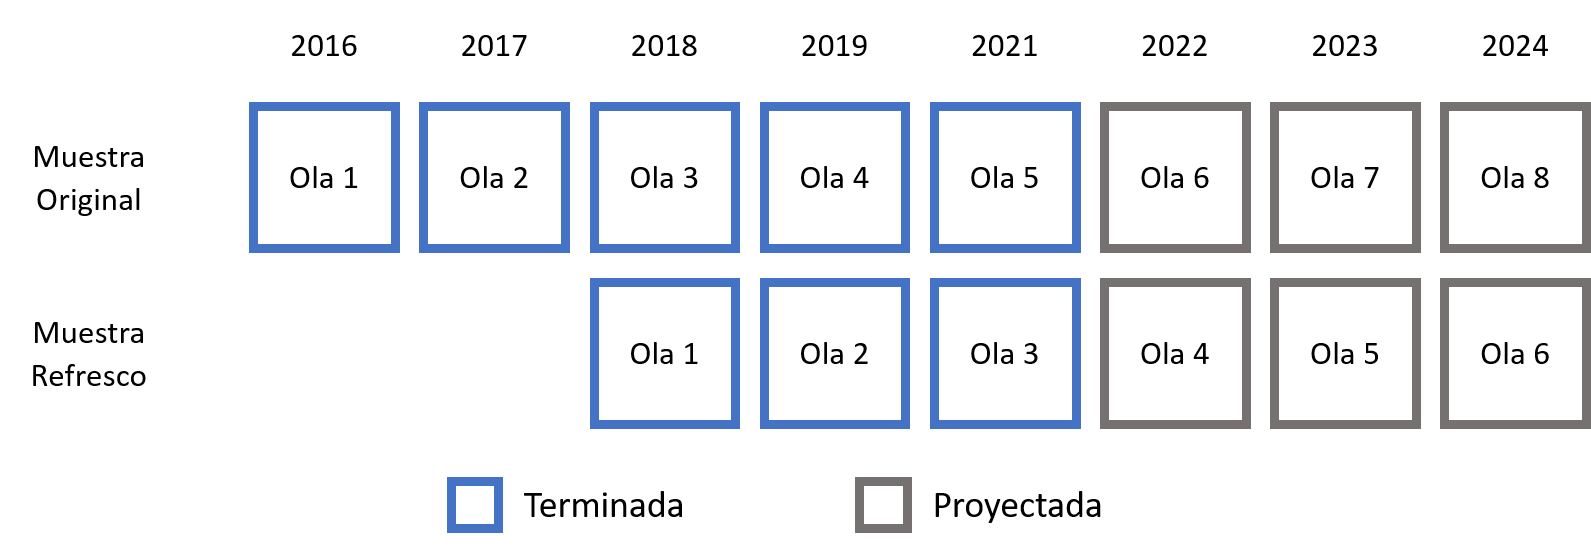
\includegraphics[width=22.1in]{1_input/imagenes/olas_elsoc}

\begin{itemize}
\item
  Marco Muestral: Marco de muestreo de manzanas del pre-censo 2011
\item
  Diseño Muestral: Probabilístico, estratificado (por tamaño de ciudades), por conglomerados y multietápico
\item
  Unidades de Muestreo: Primero se eligen ciudades (UPM), luego manzanas (USM), y sub-bloques y viviendas (UTM). La unidad final de selección es la persona
\end{itemize}

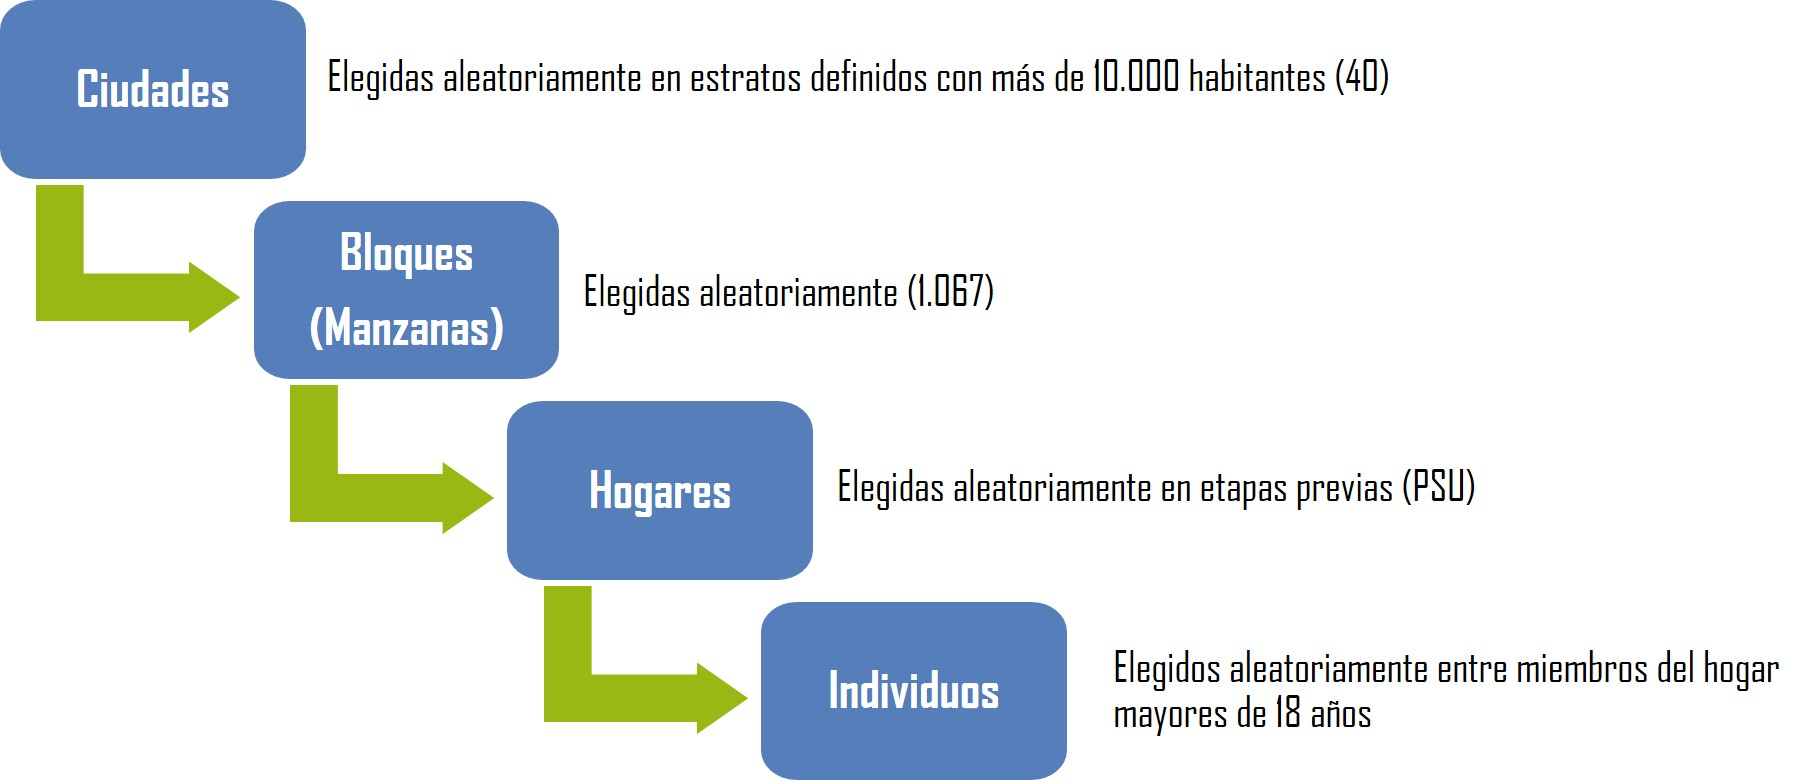
\includegraphics[width=25.24in]{1_input/imagenes/etapas_seleccion}

\textbf{Organismo Ejecutor}: Consultora Stephanie Eckman y Centro de Inteligencia Territorial (CIT) de la Universidad Adolfo Ibáñez

\hypertarget{caracteruxedsticas-del-levantamiento-de-datos}{%
\section{Características del levantamiento de datos}\label{caracteruxedsticas-del-levantamiento-de-datos}}

\begin{itemize}
\item
  Formato de aplicación: Cuestionario estructurado. Levantamiento en formato CAPI (Encuesta presencial con asistencia de tablet). Excepcionalmente se cambió a formato CATI (Encuesta telefónica con asistencia de tablet) durante 2021, debido a contingencia COVID-19
\item
  Período de Aplicación: entre Julio y Noviembre de cada año. Debido al estallido social, la cuarta medición se aplicó entre el 21 de noviembre de 2019 y el 9 de marzo de 2020. Debido a la pandemia, la quinta medición se aplicó entre el 29 de enero de 2021 y 12 de julio de 2021
\item
  Instrumento: Cuestionario compuesto por preguntas cerradas de carácter simple y múltiple junto a algunas preguntas abiertas. Combina módulos de preguntas permanentes (medidas en todas las olas) y otras intercaladas entre olas
\item
  Cobertura Temática: Contiene siete módulos temáticos: Territorio, Redes y actitudes sociales, Ciudadanía y democracia, Desigualdad y legitimidad, Conflicto social, Salud y bienestar y Caracterización sociodemográfica
\item
  Incentivos a la participación: Entrega de incentivos monetarios para el encuestado (\$ 6.000 CLP) y de material sobre el estudio (ELSOC y COES). Acciones de seguimiento basadas en la información de contacto (correo electrónico para cumpleaños y días festivos)
\item
  Entrenamiento de entrevistadores: Contratación de entrevistadores con experiencia en encuestas complejas y/o longitudinales. Capacitación centralizada y presencial para coordinadores de campo y un subconjunto de entrevistadores en Santiago (incluidos ejercicios prácticos para la implementación del cuestionario, uso de tabletas y protocolo de contacto). Actividades adicionales en otras regiones de Chile. Diseño de un Manual de entrevistador especializado para el proyecto
\item
  Operaciones de Control y Supervisión: Coordinadores de campo supervisan el trabajo de entrevistadores, verificando el número de visitas, el contacto, la identidad del participante y preguntas claves. Organismo ejecutor realiza una supervisión interna de al menos el 10\% de la muestra (entrevistando nuevamente a algunos encuestados), verificando la duración y la respuesta de los participantes
\end{itemize}

\textbf{Organismo Ejecutor}: Levantamiento a cargo de Centro Micro Datos (CMD) de la Universidad de Chile

\hypertarget{atriciuxf3n-de-la-muestra}{%
\chapter{Atrición de la muestra}\label{atriciuxf3n-de-la-muestra}}

El diseño de ELSOC contempló entrevistar a 3.000 personas en su muestra original y 1.500 en la muestra refresco. Sin embargo, es habitual que en encuestas panel se reduce el número de participantes, dado que algunos optan voluntariamente por dejar de participar y otras personas no pueden ser recontactadas. Este fenómeno es conocido como atrición, y pueden tener efectos nocivos sobre la utilidad de los datos longitudinales. En el caso de ELSOC, la tasa de atrición es comparativamente baja en comparación a otros estudios similares, por lo que no se considera al momento un problema significativo. A pesar de esto, el año 2018 se introduce una muestra refresco para contraarrestar el efecto de la atrición.

El año 2021, la atrición presenta un alza importante debido a la mayor dificultad que implica el levantamiento durante la pandemia de COVID-19 y al cambio de modalidad.

\begin{table}[H]
\centering\begin{table}[H]
\centering
\begin{tabular}[t]{c|c|c|c|c}
\hline
\multicolumn{1}{c|}{ } & \multicolumn{2}{c|}{Muestra original} & \multicolumn{2}{c}{Muestra refresco} \\
\cline{2-3} \cline{4-5}
Medición & Muestra lograda & Atrición & Muestra lograda & Atrición\\
\hline
2016 & 2 927 &  &  & \\
\hline
2017 & 2 473 & 15.5\% &  & \\
\hline
2018 & 2 229 & 9.9\% & 1 519 & \\
\hline
2019 & 2 153 & 3.4\% & 1 264 & 16.8\%\\
\hline
2021 & 1 739 & 19.2\% & 1 001 & 20.8\%\\
\hline
\end{tabular}
\end{table}
\end{table}

\hypertarget{foco-en-el-cambio-individual}{%
\chapter{Foco en el cambio individual}\label{foco-en-el-cambio-individual}}

Radiografía del Cambio Social tiene como objetivo fundamental caracterizar la estabilidad y el cambio en opiniones, actitudes y conductas de los participantes a lo largo del tiempo, enfocándose en distintas dimensiones de la cohesión y conflicto en Chile.

Para el logro de dicho objetivo, el presente reporte se centrará en un subconjunto de participantes del estudio: los 1.513 entrevistados y entrevistadas que participaron en las cinco olas de ELSOC (por lo tanto, todos son parte de la muestra original). Dicha submuestra será la base empírica de los hallazgos expuestos en las siguientes secciones.

A continuación se describe a este grupo de participantes según los mismos atributos sociodemográficos (sexo, edad, educación, zona de residencia y religión), considerando la primera medición. Todos los resultados presentados incorporan el diseño muestral complejo de la encuesta.

\textbf{Nota 1:} El promedio de edad de los participantes se ha incrementado entre estos años. También hay evidencia de un descenso en la identificación religiosa al comparar distintos años del estudio. Las otras variables no presentan variaciones relevantes a lo largo del tiempo.

\textbf{Nota 2:} Se utiliza el ponderador muestral ajustado a población regional y sexo, estrato y conglomerado muestral.

\hypertarget{nota-explicativa}{%
\section{Nota Explicativa}\label{nota-explicativa}}

A continuación, se presentan los principales resultados de la encuesta ELSOC elaborados por investigadores del Centro de Conflicto y Cohesión Social (COES). Dada la diversidad de temas que son abordados en la encuesta, los investigadores colaboradores utilizaron diversos enfoques teóricos y herramientas empíricas en su análisis. Sin embargo, en Radiografía del Cambio Social se han definido una serie de criterios comunes para el desarrollo de resultados empíricos:

\begin{itemize}
\tightlist
\item
  Foco en la evolución y cambio en las actitudes de la población, aún cuando en ocasiones se analizan preguntas incluidas en una o dos olas del estudio.
\item
  Uso de pruebas estadísticas específicas para el análisis longitudinal.
\item
  Utilización de submuestra de 1.513 participantes del estudio presentes en las cinco mediciones (2016, 2017, 2018, 2019 y 2021).
\item
  Tamaños muestrales reportados menores se explican exclusivamente por no respuesta a ítemes específicos.
\item
  Utilización del diseño muestral complejo (ponderador muestral ajustado a población regional y sexo, estrato y conglomerado muestral) en el desarrollo de figuras descriptivas y pruebas inferenciales.
\end{itemize}

\textbf{Levantamiento durante COVID-19}

\hypertarget{movimientos-sociales-y-acciones-colectivas}{%
\chapter{Movimientos Sociales y Acciones Colectivas}\label{movimientos-sociales-y-acciones-colectivas}}

\hypertarget{ciclo-de-movilizaciuxf3n-poluxedtica-y-estallido-social}{%
\section{Ciclo de movilización política y estallido social}\label{ciclo-de-movilizaciuxf3n-poluxedtica-y-estallido-social}}

\hypertarget{cuuxe1l-es-el-movimiento-social-que-usted-muxe1s-valora-de-esta-lista-seguxfan-ola-del-estudio}{%
\subsection{1.1 ¿Cuál es el movimiento social que usted más valora de esta lista? Según ola del estudio}\label{cuuxe1l-es-el-movimiento-social-que-usted-muxe1s-valora-de-esta-lista-seguxfan-ola-del-estudio}}

\hypertarget{frecuencia-de-respuesta-en-ninguno-ante-la-pregunta-cuuxe1l-es-el-movimiento-social-que-usted-muxe1s-valora-de-esta-lista-seguxfan-posiciuxf3n-poluxedtica}{%
\subsection{1.2 Frecuencia de respuesta en ``ninguno'' ante la pregunta ¿Cuál es el movimiento social que usted más valora de esta lista? según posición política"}\label{frecuencia-de-respuesta-en-ninguno-ante-la-pregunta-cuuxe1l-es-el-movimiento-social-que-usted-muxe1s-valora-de-esta-lista-seguxfan-posiciuxf3n-poluxedtica}}

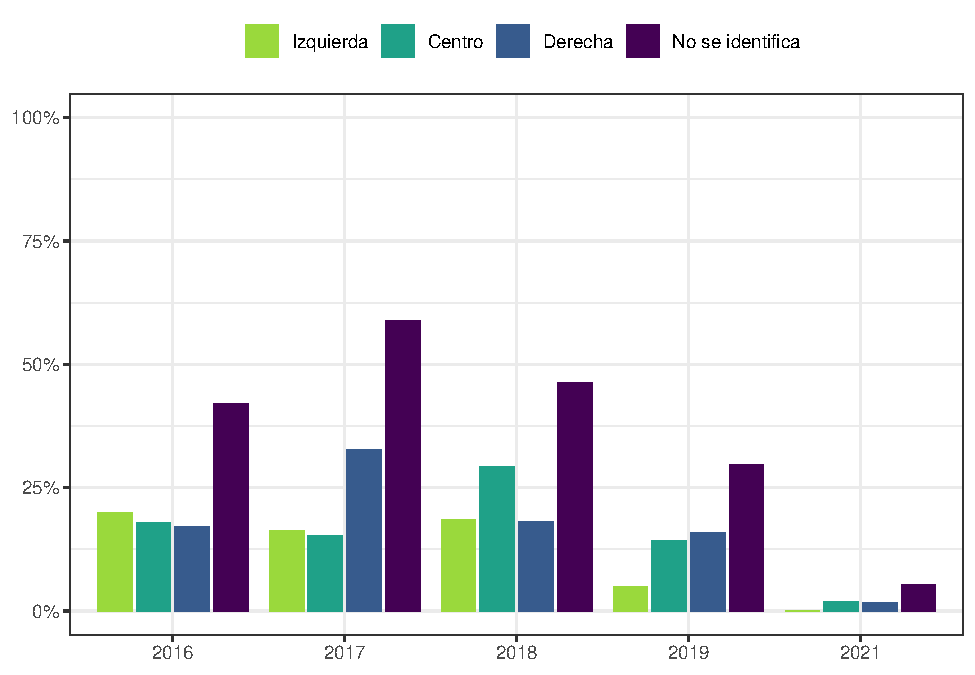
\includegraphics{reporte-elsoc_files/figure-latex/unnamed-chunk-7-1.pdf}

\hypertarget{alluvial-de-movimiento-social-que-muxe1s-valora}{%
\subsection{1.3 Alluvial de movimiento social que más valora}\label{alluvial-de-movimiento-social-que-muxe1s-valora}}

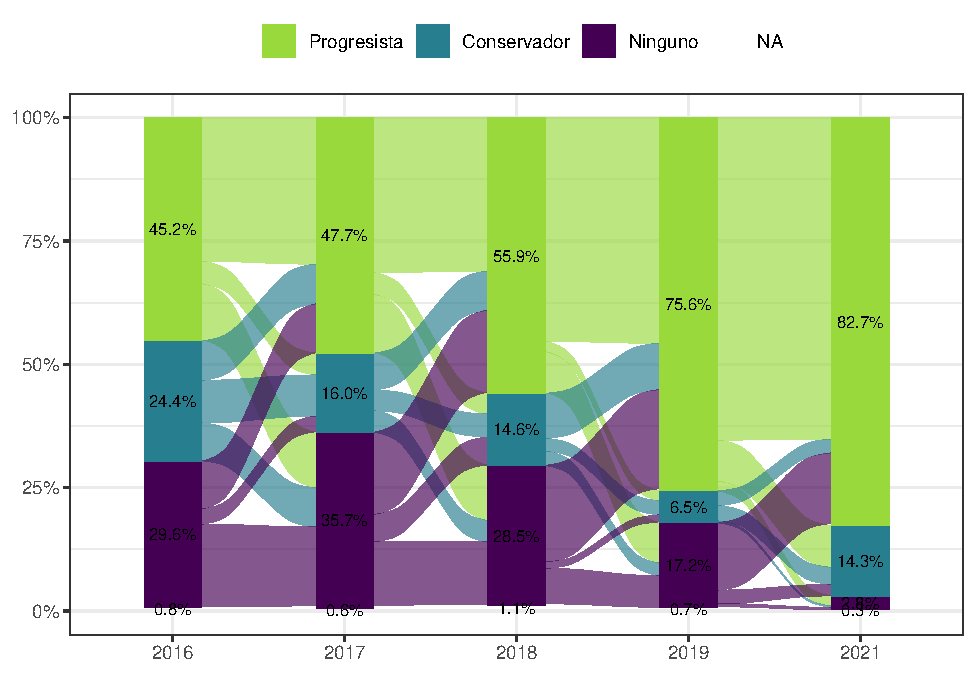
\includegraphics{reporte-elsoc_files/figure-latex/unnamed-chunk-8-1.pdf}

La determinación entre las categorías ``Progresista'' y ``Conservador'' se hizo en base a la siguiente agrupación de movimientos sociales:

Progresista: Movimiento social de apoyo a la causa estudiantil, Movimiento social de apoyo a demandas laborales, Movimiento social de grupos ambientalistas, Movimiento social de apoyo a las demandas indígena, Movimiento social de apoyo a la diversidad sexual, Movimiento feminista o de apoyo a la igualdad de género, Movimiento por el cambio al sistema de pensiones, Estallido social del 18 de Octubre de 2019

Conservador: Movimiento social provida o antiaborto, Movimiento social antidelincuencia

\hypertarget{descriptivos-generales}{%
\subsection{1.4 Descriptivos generales}\label{descriptivos-generales}}

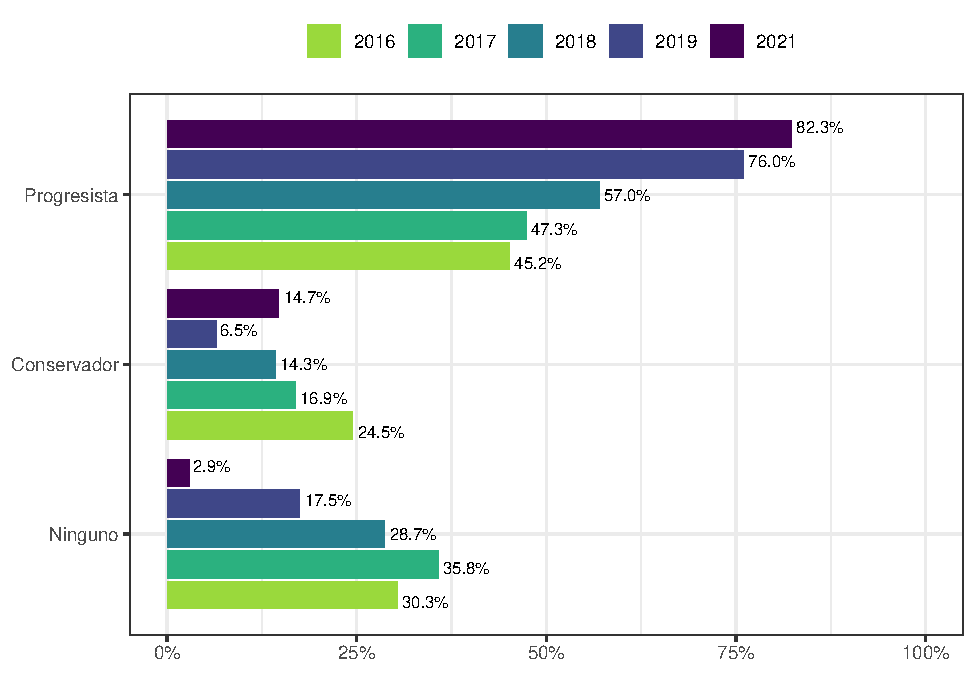
\includegraphics{reporte-elsoc_files/figure-latex/unnamed-chunk-9-1.pdf}

\hypertarget{cambios-en-la-valoraciuxf3n-de-movimientos-sociales-seguxfan-posiciuxf3n-poluxedtica}{%
\subsection{1.5 Cambios en la valoración de movimientos sociales según posición política}\label{cambios-en-la-valoraciuxf3n-de-movimientos-sociales-seguxfan-posiciuxf3n-poluxedtica}}

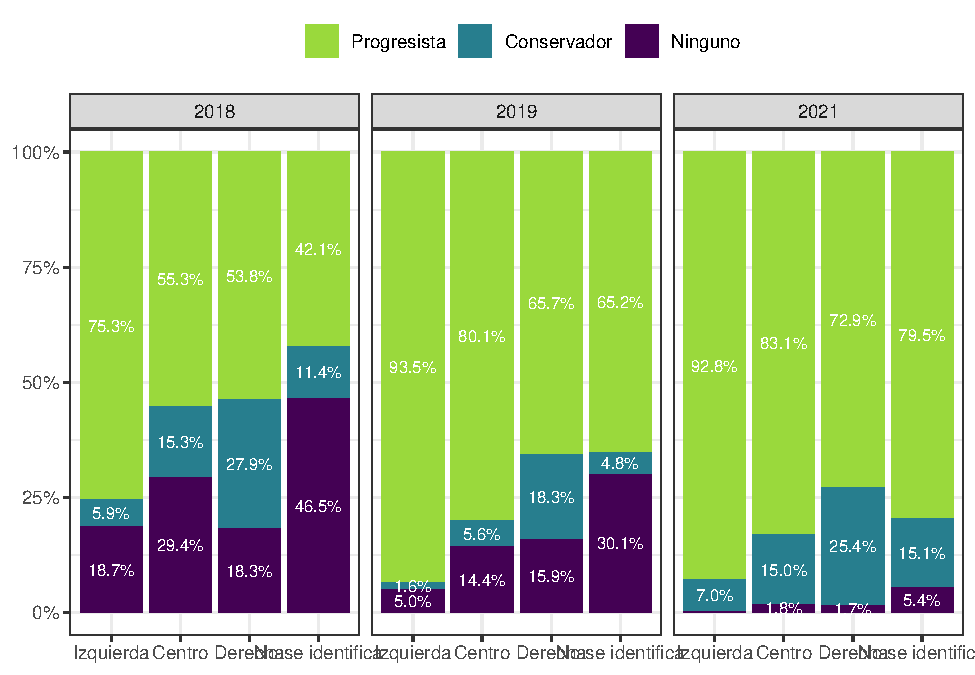
\includegraphics{reporte-elsoc_files/figure-latex/unnamed-chunk-10-1.pdf}

\hypertarget{cambios-en-la-valoraciuxf3n-de-movimientos-sociales-seguxfan-nivel-educativo}{%
\subsection{1.6 Cambios en la valoración de movimientos sociales según nivel educativo}\label{cambios-en-la-valoraciuxf3n-de-movimientos-sociales-seguxfan-nivel-educativo}}

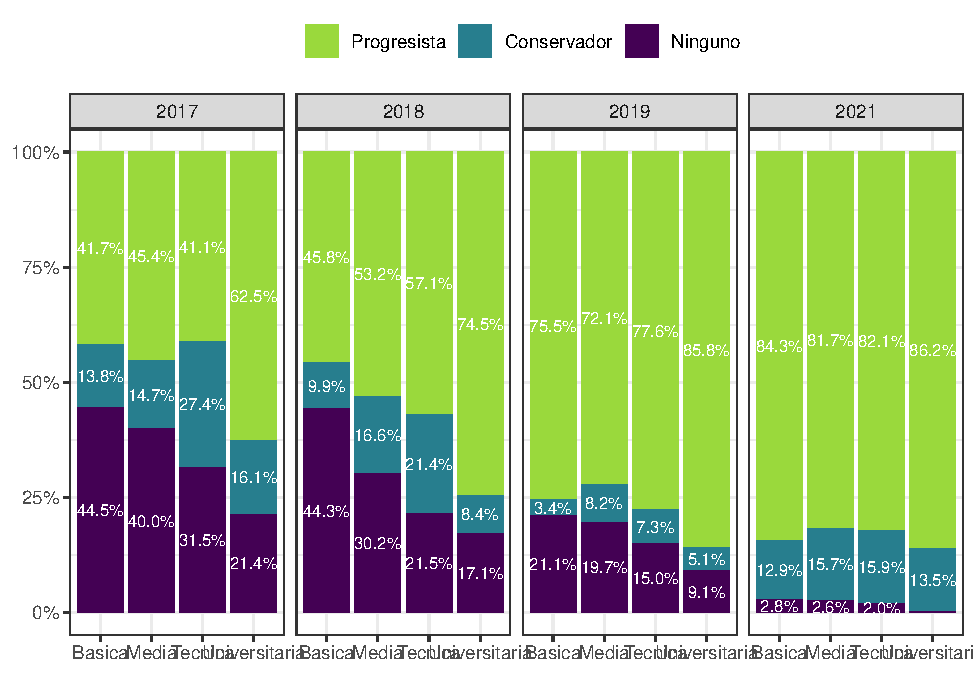
\includegraphics{reporte-elsoc_files/figure-latex/unnamed-chunk-11-1.pdf}

\hypertarget{valoraciuxf3n-de-movimientos-sociales-segun-segun-participacion}{%
\subsection{1.7 Valoración de movimientos sociales segun segun participacion}\label{valoraciuxf3n-de-movimientos-sociales-segun-segun-participacion}}

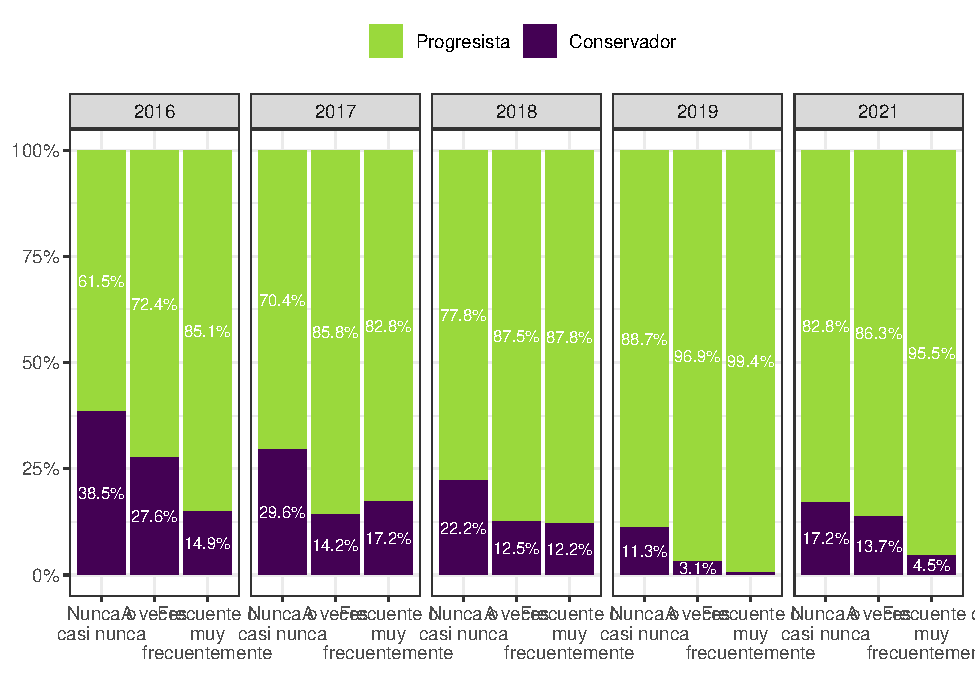
\includegraphics{reporte-elsoc_files/figure-latex/unnamed-chunk-12-1.pdf}

\hypertarget{frecuencia-de-participaciuxf3n-en-movimientos-sociales-seguxfan-ola-de-encuesta.-porcentaje-que-responde-frecuentemente-o-muy-frecuentemente}{%
\subsection{1.8 Frecuencia de participación en movimientos sociales, según Ola de encuesta. Porcentaje que responde Frecuentemente o Muy frecuentemente}\label{frecuencia-de-participaciuxf3n-en-movimientos-sociales-seguxfan-ola-de-encuesta.-porcentaje-que-responde-frecuentemente-o-muy-frecuentemente}}

\hypertarget{confianza-en-instituciones}{%
\section{Confianza en instituciones}\label{confianza-en-instituciones}}

\hypertarget{bastante-o-mucha-confianza-en-ella-presidentea-de-la-repuxfablica-el-gobierno-y-el-congreso-nacional-seguxfan-auxf1o}{%
\subsection{1.9 Bastante o Mucha confianza en el/la Presidente(a) de la República, el Gobierno y el Congreso Nacional según año}\label{bastante-o-mucha-confianza-en-ella-presidentea-de-la-repuxfablica-el-gobierno-y-el-congreso-nacional-seguxfan-auxf1o}}

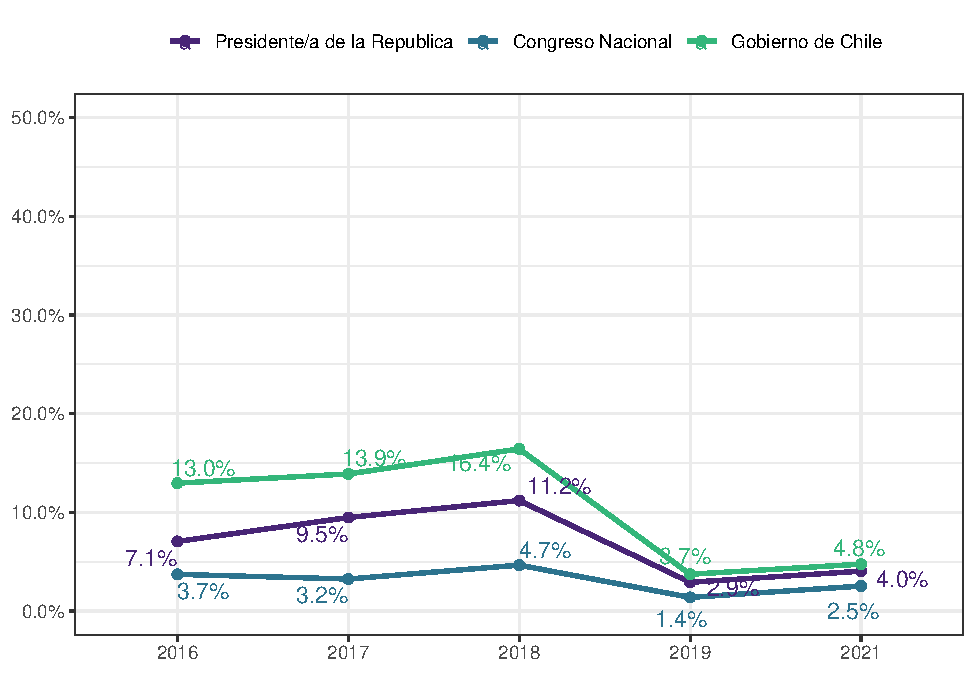
\includegraphics{reporte-elsoc_files/figure-latex/unnamed-chunk-14-1.pdf}

\hypertarget{bastante-o-mucha-confianza-en-carabineros-el-poder-judicial-y-en-partidos-poluxedticos-seguxfan-auxf1o}{%
\subsection{1.10 Bastante o Mucha confianza en Carabineros, el Poder Judicial y en Partidos Políticos según año}\label{bastante-o-mucha-confianza-en-carabineros-el-poder-judicial-y-en-partidos-poluxedticos-seguxfan-auxf1o}}

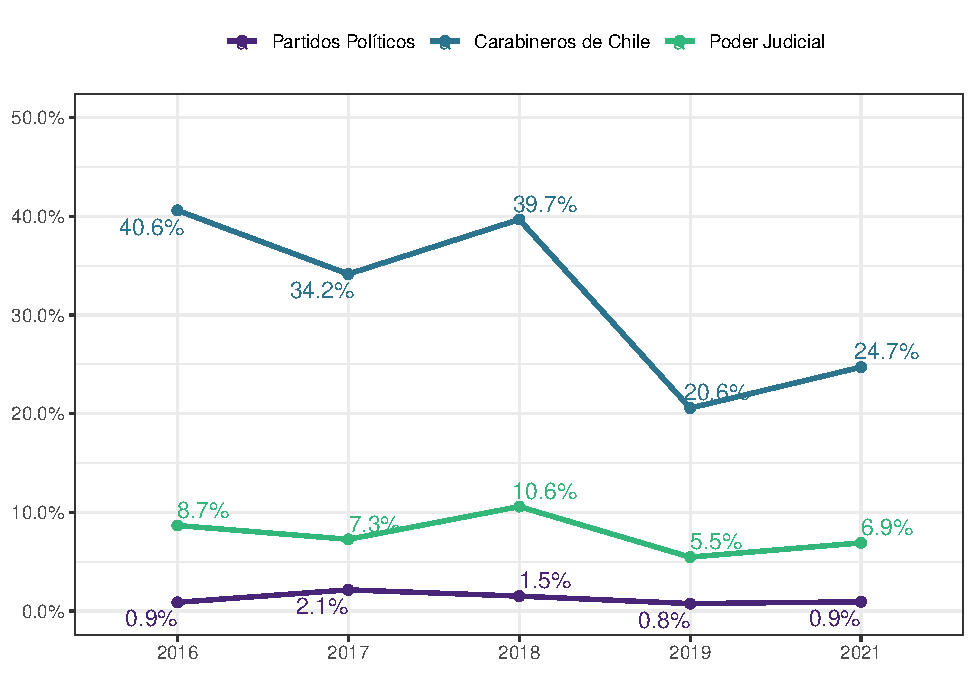
\includegraphics{reporte-elsoc_files/figure-latex/unnamed-chunk-15-1.pdf}

\hypertarget{identificaciuxf3n-poluxedtica}{%
\chapter{Identificación Política}\label{identificaciuxf3n-poluxedtica}}

\hypertarget{identificaciuxf3n-poluxedtica-1}{%
\section{Identificación política}\label{identificaciuxf3n-poluxedtica-1}}

\hypertarget{identificaciuxf3n-poluxedtica-por-ola}{%
\subsection{2.1 Identificación política por ola}\label{identificaciuxf3n-poluxedtica-por-ola}}

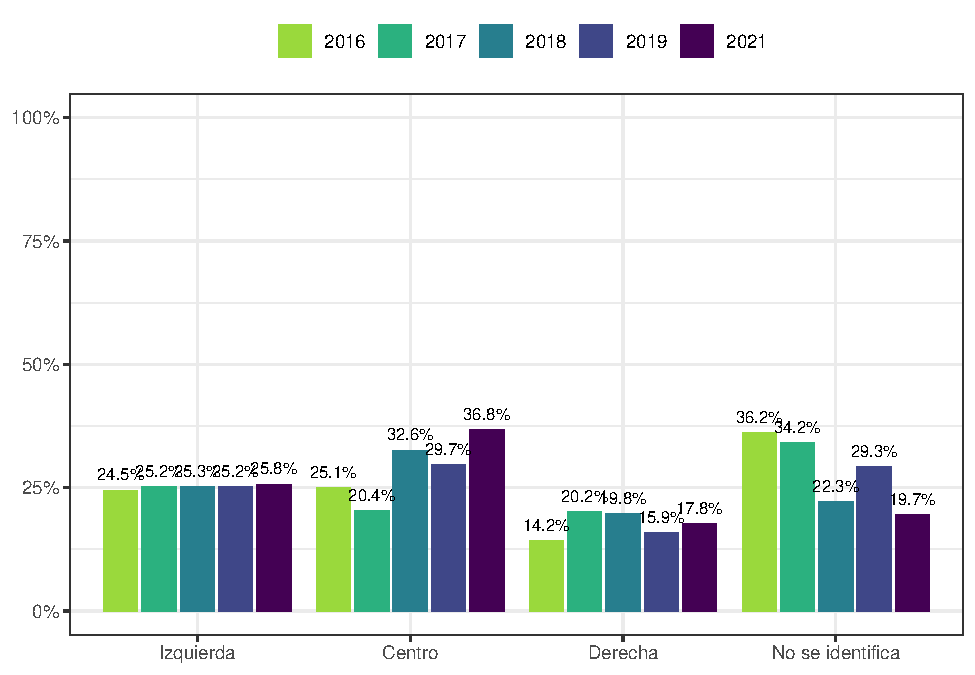
\includegraphics{reporte-elsoc_files/figure-latex/unnamed-chunk-16-1.pdf}

\hypertarget{alluvial-de-cambios-de-identificaciuxf3n-poluxedtica}{%
\subsection{2.2 Alluvial de cambios de Identificación política}\label{alluvial-de-cambios-de-identificaciuxf3n-poluxedtica}}

\hypertarget{de-acuerdo-o-totalmente-de-acuerdo-con-la-cuarentena-seguxfan-identificaciuxf3n-poluxedtica-el-auxf1o-2021}{%
\subsection{2.3 De acuerdo o Totalmente de acuerdo con la cuarentena según identificación política el año 2021}\label{de-acuerdo-o-totalmente-de-acuerdo-con-la-cuarentena-seguxfan-identificaciuxf3n-poluxedtica-el-auxf1o-2021}}

\hypertarget{grado-de-acuerdo-con-actividad-econuxf3mica-versus-salud-puxfablica-seguxfan-identificaciuxf3n-poluxedtica-el-auxf1o-2021}{%
\subsection{2.4 Grado de acuerdo con actividad económica versus salud pública según identificación política el año 2021}\label{grado-de-acuerdo-con-actividad-econuxf3mica-versus-salud-puxfablica-seguxfan-identificaciuxf3n-poluxedtica-el-auxf1o-2021}}

\hypertarget{grado-de-acuerdo-con-el-aborto-seguxfan-identificaciuxf3n-poluxedtica}{%
\subsection{2.6 Grado de acuerdo con el aborto según identificación política}\label{grado-de-acuerdo-con-el-aborto-seguxfan-identificaciuxf3n-poluxedtica}}

\hypertarget{grado-de-acuerdo-con-la-capitalizacion-individual-pensiones-seguxfan-identificaciuxf3n-poluxedtica}{%
\subsection{2.7 Grado de acuerdo con la capitalizacion individual pensiones según identificación política}\label{grado-de-acuerdo-con-la-capitalizacion-individual-pensiones-seguxfan-identificaciuxf3n-poluxedtica}}

\hypertarget{grado-de-acuerdo-con-las-restricciones-de-ingreso-de-migrantes-seguxfan-identificaciuxf3n-poluxedtica}{%
\subsection{2.8 Grado de acuerdo con las restricciones de ingreso de migrantes según identificación política}\label{grado-de-acuerdo-con-las-restricciones-de-ingreso-de-migrantes-seguxfan-identificaciuxf3n-poluxedtica}}

\hypertarget{actitudes-hacia-la-democracia}{%
\chapter{Actitudes hacia la democracia}\label{actitudes-hacia-la-democracia}}

\hypertarget{apoyo-a-la-democracia}{%
\section{Apoyo a la Democracia}\label{apoyo-a-la-democracia}}

\hypertarget{con-cuuxe1l-de-las-siguientes-frases-estuxe1-usted-muxe1s-de-acuerdo}{%
\subsection{3.1 ¿Con cuál de las siguientes frases está usted más de acuerdo?}\label{con-cuuxe1l-de-las-siguientes-frases-estuxe1-usted-muxe1s-de-acuerdo}}

\hypertarget{insatisfacciuxf3n-con-la-democracia-por-ola}{%
\subsection{3.2 Insatisfacción con la democracia por ola}\label{insatisfacciuxf3n-con-la-democracia-por-ola}}

\begin{verbatim}
## 1 variables were not found in the dataset: c01
\end{verbatim}

\begin{verbatim}
##     [1]    1    1    1    1    2    1    3    3    1    4    3    1    1    1
##    [15]    2    3    1    1    1    1    1    4    1    1    3    1    1    4
##    [29]    1    3    3    2    1    1    3    1    1    1    1    2    4    1
##    [43]    1    1    2    2    1    1    3    2    1    2    2    1    1    2
##    [57]    3    3    3    1    2    1    2    1    1    2    1    2    2    4
##    [71]    1    3    1    1    1    1    1    2    2    1    2    3    1    1
##    [85]    3    4    1    1    1    1    1    1    1    1 -888    1    1    1
##    [99]    1    1    3    1    1    3    1    1    1    1    1    2    3    1
##   [113]    1    1    1    1    2    2 -888    1    3    1    1    3    2    1
##   [127] -888    1    1    1    2    1    1    1    1    1    1    2    1    1
##   [141]    3    1    1    1    2    3    1    1    1 -888    1    2    3    3
##   [155]    1    1    1    1    1    1    1    5    3    3    3    3    1    1
##   [169]    1 -888    1    1    1    1    1    1 -888    1    1 -888    3    1
##   [183]    1    1    3    1    1    1    1    1    2    4    1    2    1    1
##   [197]    1    1    1    1    3    1    1    2    1    1    1    2    1    2
##   [211]    2    3    1    3    1    1    3    2    1    3    1    2    1    4
##   [225]    1    1    2    2    1    2    3    4    1    1    2    2    1    1
##   [239]    3    1    1    5    2    2    1    1    2    3    1    3    3    1
##   [253]    1    3    2    1    2    1    1    3    3    1    3 -888    3    1
##   [267]    3    3    4    1    1    2    1    2    4    4    1    1    3    4
##   [281] -999    3    3    1    1    4    3 -888    4    1    3    2    1    1
##   [295]    5    1    2    2    2    1    3    2    3    4 -888    1    5 -888
##   [309]    1    4    3    4    2    1    1    1    1    5    2    3    1    1
##   [323]    2    1    2    2    2    1    1    1 -888    1    2    2    1    1
##   [337]    3    1    5    2    3    2    3    1    2    2    3    1    2    2
##   [351]    1    3    1    1    2    1    1    3    2    3    3    1    4    1
##   [365]    1    1    2    1    1    2    1    1    2    1    2    3    4    1
##   [379]    2    3    1    1    3    1    3    2    3    1    3    1    1    1
##   [393]    3    5    2    4    1    3    2    1    1    1    5    1    2    3
##   [407]    1    3    2    1    1    2    5    3    1    2    4    1    1 -888
##   [421]    3    2    2    2    2    4    1    1    3    3    2    1    3    2
##   [435]    2    3    1    2    2    2    3    1    1    1    1    2    1    1
##   [449]    1    1    2    1    2    4    2    2    3    3    1    1    2    3
##   [463]    3 -888    1    2    1    1    2    2    1    2    1    2    1    2
##   [477]    5    3    1    1    3    4    1    1    3    2    2    1    3    2
##   [491]    5    1    1    1    5    1    4    2    1    1    1    1    3    2
##   [505]    2    1    1    1    3    1    2    2    3    1    2    1    3    4
##   [519]    3    1    2    3    4    2    1    4    2    1    1    5    2    1
##   [533]    3    4    2    1    1    1    1    2    2    2 -999    1    2    4
##   [547]    2    4    1    3    3    4    1    1    3    2    2    3    2    3
##   [561]    3    1    1    3    1    4    4    1    1    1    4    3    1    1
##   [575]    2    4    1    2    3    1    2    4    2    1    3    1    2    2
##   [589]    1    1    4    2    4    1    2    2    1    1    3    3    2    1
##   [603]    1    3    2    1    1    1    2    1    1    2    2    1    3    3
##   [617]    2    3    3    3    2    3    5    3    1    2    1    1    2    1
##   [631]    2    2    3    3    3    2    2    1    2    3    1    3    1    4
##   [645]    3    2    1    1    2    1    1    1    2    1    1    3    2    2
##   [659]    2    1    2    1    1    4    3    2    3    2    2    2    3    2
##   [673]    2    1    1    1    2    3    4    1    1    3    1    1    2    1
##   [687]    3    2    3    1    3    4    2    3    1 -888    3    3    3    3
##   [701]    1    1    1    1    2    5    3    4    1    2    2    4    3    3
##   [715]    1    1    1    1    1    1    1    2    5    1    1    2    1    1
##   [729]    3    1    1    1    1    1    4    1    1    5    1    1    1    2
##   [743]    1    1    3    1    1    4    2    2    2    1    1    1    1    1
##   [757]    1    1    2    1    3    1    1    3    1    1    1    5    1    3
##   [771]    1    3    5    1    1    2    3    2    2    2    1    1    2    1
##   [785] -888    1    2    2    1    1    2    3    1    3    1    2 -888 -888
##   [799]    3    3    2    2    1    1    3    1    3    1    1    2    1    4
##   [813]    3    1    1    1    2    1    3    3    4    4    3    4    3    2
##   [827]    2    3    2    3    5 -888    3    3    2    5    2    2    3    1
##   [841]    2    4    3    1    3    1    2    2    1    2    1    3    2    4
##   [855]    1    3    1    3    2    3    3    1    1    1    3    2    1    3
##   [869]    1    1    3 -888    2    1    3    1    1    3    3    2    1 -888
##   [883]    1    1    3    3    2 -999    1    2    1    1    1    1    1    1
##   [897]    2 -888 -888    3    2    3    1    3    1    3    3    1 -888    2
##   [911]    3    1    4    1    1    2    3    2    5    2    3    2    1    4
##   [925]    5    3    1    1    2    2    1    1    1 -888    2    3    1    1
##   [939]    2    3    1    2    4    1    3    1    1    3    4    1    1    1
##   [953]    3    2    3    2    2    2    1    4    2    1    3    3    1    2
##   [967]    1    3    3    1    2    1    1    2    5    3    1    3    3    2
##   [981]    3    3    1 -888    3    3    4    2    2    2    3    2    3    3
##   [995]    1    3    3    1    1    1    1    2    1 -888    2    1    2    1
##  [1009]    1    3    3    1    1    2 -888    1    1    1    1    3    2    2
##  [1023]    4    1    1    2    3    3    1    1    1    1    4    2    2    3
##  [1037]    2    2    1    4    1    2    5    3    3    3    2    1    2    3
##  [1051]    1 -888    2    2    1    1    2    3    1    2    1    1    1    2
##  [1065]    3    1    1    3    2    2    1 -888 -888    2    2    1    1    1
##  [1079]    1    1    3    3    3    1    1    1 -999    3    1    2    1    1
##  [1093]    2    1    2    3    3    2    3    1    3    2    1 -888    1    2
##  [1107]    1    1 -888 -999    1    1    3    3    1    3    3 -888    1    3
##  [1121]    1    3    4    1    2    3    2    2 -888    2    2    1 -888    2
##  [1135]    2    3    1    1    2    1    1    2    1    2    1    3    2    3
##  [1149] -888    1    2    3    2    2    2 -888    3    1 -888    1    1    2
##  [1163]    2    4 -888    3    1    1    1    3    3    1    2    4    1    1
##  [1177] -888 -888    1 -999    1    3    2    1    1    1    1    2    3    4
##  [1191] -888    1    2    2    2    1    1    1    3 -888 -888 -888    3    2
##  [1205] -888    1    2    1    5    3    1    4    1    2    2    1    1    1
##  [1219]    1    3    2    3    1    4    1    1    2 -888    1    1    5    2
##  [1233] -888    1    2    1    2    1 -999    1    2    1    1    1    3    3
##  [1247]    1    1    5    4    1    1    1    2    2    1    1    3    1    3
##  [1261]    2    3    1    2    1    1    1    1    1    2    1    2    1    1
##  [1275]    3    1 -888 -999    2 -999    1    1    4    3    1    1    2    2
##  [1289]    1    2    1 -888    1    1    1    1 -999    5 -999    3    1    3
##  [1303] -999    2    2    2    1    2    3    5    2    2    3    2 -888    1
##  [1317]    1    3    3    1    2    2    1    2    1    1    1    2    1    2
##  [1331]    1    1    1    1    3    1 -888    1    1    1    1    1    3 -888
##  [1345]    2    3 -888    3    3    2    2    2    1    3    1    1    5    1
##  [1359]    1    3    1    1    1    2    1    2    1    2    1    4    1    1
##  [1373]    3    2    3    3    3    1    1 -888    3    1    1    1    4    3
##  [1387]    3    3    1 -888    2    2    4    2 -888    2    3 -888    1 -999
##  [1401]    1    3    2    3 -888    1 -888    1 -888    2    3    3    3    2
##  [1415]    2    1 -999    1    4    3    2    1    2    1    3    3    4    2
##  [1429]    5    2    1    3    1    2 -888    2    1    2    1    1    3    3
##  [1443]    1    1    3    2    1    1    2    1    1    4    3    3    2    1
##  [1457]    1    1    1    3    2    1    1    1    1    3    1    2    1    1
##  [1471]    1    1    1    1    1    1    1    2    3    1    1    1    1    1
##  [1485]    1    2    1    1    3    3    1    1    1    1    2    1    1    2
##  [1499]    1 -888    2    1    2    1    2    4    2    1    1    3    4    1
##  [1513]    3    2    1    1    1    1    1    1    1    3    2    2    2    2
##  [1527]    1    2    1    1    2    1    1    1    3    4    2    1    3    1
##  [1541] -999    1    1    1    1    1    1    2    3    2    2    3    2    1
##  [1555]    1    2    1    1    2    3    3    2    3    3    1    4    4    4
##  [1569]    2    5    1    5 -888    1    4    2    1    2    3    1 -888 -888
##  [1583]    2    3    1    1    1    1    1    1    1    4    4    2    1    1
##  [1597]    5    1    2 -888    2    1    1    1    2    3    1    4    1    1
##  [1611]    1    1    1    1    1    4    1    1    1    4    1    3    1    2
##  [1625]    1    1    1    1    1    2    1    1    1 -888    2    2    2    4
##  [1639]    2    1    2    4    1    3    2    4    2    1    3    3    3    4
##  [1653]    1    1    1    1    2    1    4    4    3    3    3    3    4    3
##  [1667]    3    2    1    1    1    2    2    1    1    1    1    3    1    5
##  [1681]    4    1    1    1    1    2    2    1    4    3    3    1    3    3
##  [1695]    5    1    4    3    4    4    3    3    3    3    3    3    1    2
##  [1709]    2    2    1    1    1    1    2    1    1    4    2    1    2    1
##  [1723]    3    2    4    4 -888    2    4    3    1    1    3    2    2    2
##  [1737]    1    4    2    3    1    5    4    1    1    3    2    2    1    1
##  [1751]    1    2    2    2    3    1    2    1    1    1    2    1 -888    2
##  [1765]    3    3    4    2    4    1    4    3    4    4    1    3    1    4
##  [1779] -888    1    5    1    4    1    1 -999    1    3    3 -888    2    2
##  [1793]    3    1    1    2    3    1    1    1    1    1    1 -888    4    1
##  [1807]    1    1    1    1    2    1    4    2    3    1    1    1    1    2
##  [1821]    1    1    1    4    1    2    2    2    4 -888    3    3    3    3
##  [1835]    2    3    3    3    2    3    3    3    1    2    2    2    2    3
##  [1849]    2    3    3    2    1    2    3    4    2    3    1    2    2    2
##  [1863] -888 -888    1    2    3    2    1    2    2    3    2    2    3    2
##  [1877]    2    1    5    2    2 -888    1    2    3    2    1    2    1    1
##  [1891]    1    1    2    1    1    1    2    3    3    4    3    3    4    2
##  [1905]    4    1    2    1    1    2    3    1    4    5    1    2    1    2
##  [1919]    3    1    1    1    3    1    1    1    2    1    3    1    3    2
##  [1933]    1    4    1    2    3    1    3    1    2    2    2    1    3    1
##  [1947]    4    2    1    3    2    1    1    1    3    2    2    3    4    4
##  [1961]    1    5    2    2    2    5    3    3    1    2    3    3    3    2
##  [1975]    3    1    1    2    2    2    2    3    1    3    3    2    3    3
##  [1989]    1    1    3    3    5    1    1    1    1    2    1 -888    1    4
##  [2003]    1    3    2    3    3    1    1    3    2    4    3    2    3    1
##  [2017]    1    2    2    3    3    1    2    1    3    1    3    3    2    3
##  [2031]    2    1    3    1    3    1    3    3 -999    3    1    3    2    1
##  [2045]    1    1    1    3    2    1    3    4    1    1 -888    1    3    1
##  [2059]    3    1    1    3    1    3    1    2    1    1    2    1    3    4
##  [2073]    1    1    2    5    3    3    1    2    1    1    2    1    1    3
##  [2087]    4    1    4    1    1    2    2    2    3    3    2    1    4    3
##  [2101]    1    1    1    1    4    3    3    2    2    2    1    1    2    2
##  [2115]    1    1    1    2    3    1 -888    4    1 -888    1 -888    1    3
##  [2129]    2    1    1    1    2    1    2    4    3    1    1    2    2    1
##  [2143]    2    3    2    1    1    3    2    2    2    1    3    3    3    1
##  [2157]    2    5    1    2    2    2    1    2    3    2    1    1    3    3
##  [2171]    5    2    1    2    1    3    1    2    3    2    4    2    3    1
##  [2185] -888    1 -888    2    1    1    1    4    1    1    1    5    3    1
##  [2199]    4    3    2    1    4    1    3    1    1    2    3    2    3    2
##  [2213]    4    2    1    1    4    4    5    4    2    5    3    1    2    1
##  [2227]    1    1    4    1    3    2    3    3    3    4    4    3    3    2
##  [2241]    2    2    2    2    2    4    3    2    2    2    2    2    1    1
##  [2255]    5    3    2    3    3    2    5    4    1    2    4    1    1    1
##  [2269]    1    1    1    1    5    5    3    3    1    1    3    3    2    3
##  [2283]    2    2    3    2    1    1    2    2    3    1    2    3    1    3
##  [2297]    3    3    4    1    1    3    3    3    1    1    4    3    1    3
##  [2311]    1    5    1    1    3    2    1    5    1    5    3    2    3    2
##  [2325]    1    3    2    3    2    3    3    2    4    3    2    2    1    1
##  [2339]    2    2    2    1    4    2    1    1    1    2    2    1    3    1
##  [2353]    1    1    4    3    2    1    1    2    2    3    2    1    1    1
##  [2367]    4    2    1    1    2    1    1    1    1    2    2    1    1    3
##  [2381]    3    2    3    4    3    1    3    2    2    2    2    1    2    2
##  [2395]    1    1    1    2    2    4    1    2    2    2    2    1    4    2
##  [2409]    2    1    3    4    5    1    2    1    2    1    1    3    3    4
##  [2423]    2    2    1    2    2    1    2    2    1    3 -888    4    1    2
##  [2437] -888    4    1    3    1    5    4    1    1    4    2    3    1    2
##  [2451]    1    2    1    1    2    1    4    3    2    1    4    3    2    1
##  [2465]    2    2    4    2    1    1    1    1    1    1    2    1    1    1
##  [2479]    1    3    3    3    3    1    1    2    1    1    1    3    2    1
##  [2493]    1    1 -888    1 -888    1 -888    2    1    1    4    1    2    1
##  [2507]    1    2    4    3    1    1    1    1 -888    2    2    1    1    3
##  [2521]    3    3    1    5    1    3    3    1    5    2    2    2    1    2
##  [2535]    4    1    3    1    4    2    2    4    2    1    4    1    1    5
##  [2549]    1    1    2    1    5    2    1    3    2    1    2    3    3    1
##  [2563]    4    1    1    4    1    1    3    1    1    2    1    2    1    3
##  [2577]    3    1    2    2    1    4    1    1 -999    4    1    3    1    3
##  [2591]    2    2    3    1    1    1    1    1    1    1    2    1    1    1
##  [2605]    1    4    4    4    4    4    1    4    1    4    1    2    2    3
##  [2619]    5    3    2    3    1    2    1    1    1    3    1    1    5    2
##  [2633]    1    2    1    2    2    1    4    3    3    1 -888    1    3    1
##  [2647]    1    2    4    3    1    4    1 -888    2    2    3 -888    1    1
##  [2661]    2    1    1    2    1    3    3    4    2    2    1    3    3    1
##  [2675]    2    3    3    3    1    2    2    3    3    5    1    1    1    3
##  [2689]    1    1    3    2    2    3    1    3    2    1    1    2    1    2
##  [2703]    2    1    1    2    1    1    2    3    4    1    1    1 -999    1
##  [2717]    1    1    1    1    3    1    1    1 -999 -999    5    3    2    1
##  [2731]    1    3    2    1    2    3    1    1    1    1    2    2    1    4
##  [2745]    4    1    3    3    3    2    3    3    1    1    3    5    1    4
##  [2759]    2    4    2    3    4    1    1    2    4 -888    3    2    2    1
##  [2773]    2 -888    4    2    5    4    3    3    4    2    1    5    5    3
##  [2787]    2    1    1    5 -888    1    1    2    1    1    1    3    3    4
##  [2801]    1    3    1    2    1    3    2    2    1    2    2    3    1    3
##  [2815]    1    1    2    1    2    1    2 -888    3    1    1    1    3    1
##  [2829]    1    3    4    1 -888 -888    5    3 -888 -888 -888    1    1 -888
##  [2843]    1    1    1    2    1    1    1    2    1    1    2    2    2    1
##  [2857]    3    1    1    1    2    3    3    1    3    1    2    1    1    2
##  [2871]    1    2    2    3    3    2    2    3    3    3    2    2 -888    2
##  [2885]    3    1    3    3    2    1    1    1    1    3 -888 -888    2    2
##  [2899]    1    2    1    3    2    2    3    1    3    3 -999    3    3    2
##  [2913]    2    1    1    2    1    2    1    1    3    1    1    2    2    1
##  [2927]    3    2    1    1    3    2    4    1    3    1    1    3    1    1
##  [2941]    2    1    3    2    3    3    3    2    2    3    1    1    2    1
##  [2955]    1    2    2    2    3    2    4    2    3    1    1    2    4    1
##  [2969]    3    1    1    1    1    3    3    2    1    2    1    1    1    3
##  [2983]    3    4    2    1    1    3    1    2    2    1    1    1    1    1
##  [2997]    1    1    1    1    3    1    2    1    1    1    3    4    3    1
##  [3011]    2    2    1    1    3    3    2    1    1    2    3    2    1    2
##  [3025]    3    1    3    3    2    1    1    1    2    2    1    1    1    1
##  [3039]    3    1    1    2    1    2    1    1    1    1    1    1    1    2
##  [3053]    2    2    1    1    1    3    3    1    1    1    1    2    1    1
##  [3067]    1    1    1    1    1    3    2    3    3    3    1    1    3    1
##  [3081]    1    2    2    1    2    1    1    1    3    2    1    2    3    3
##  [3095]    1    1    1    1    1    1    1    1    1    1    2    1    1    1
##  [3109]    1    1    1    1    3    4    1    4    2    1    2    3    2    5
##  [3123]    3    1    3    3    4    2    3    1    1    1    1    2    1    4
##  [3137]    1    4    1    4    4    3    1    5    4    2    4    2    1    2
##  [3151]    3    4    2    3    3    4    3    3    4    3    2    3    4    3
##  [3165]    4    2    3    3    4    3    3    3    3    5    2    3    3    3
##  [3179]    1    4    4    3 -888    3    3    3    4    4    3    3    4    3
##  [3193]    1    4    4    3    1    2    1    4    2    3    4    3    3    1
##  [3207]    2    1    2    2    1    2    3    3    3    1    1    2    2    3
##  [3221]    1    2    3    3    3 -888    1    1    2    2    2    1    1    4
##  [3235]    3    3    1    2    4    1    1    3    2    1    3    1    2    3
##  [3249]    1    1    3    3    2    3    1    3    3    2    3    1    1    1
##  [3263]    1    2    1    1    4    1    4    5    3    3    1    2    2    1
##  [3277]    3 -888    1    1 -888    3 -888    3    1    3    5    2    2    2
##  [3291]    2    2    2    4    1    2    1    4    4    2    2    2    2    2
##  [3305]    3    5    3    2    3    1    2    2    1    2    1    1    3    3
##  [3319]    3    2    2    2    4    2    2    2    2    2    3    3    3    1
##  [3333]    5    1    1    3    3    3    3    2    1    2    2    2    3    1
##  [3347]    1    1    2    2    1    1    1    1    1    1    5    4 -888    4
##  [3361]    1    1    1    4    4    4    3 -999 -999    3 -999    2    3 -888
##  [3375]    1    4    3    1    1    1    1    3    1    1    2    3    4    3
##  [3389]    3    3    2    1    1    1    4    2    3    4    1    1    4    3
##  [3403]    2    3    2    1    2    1 -888    1 -888    1 -888    1 -888    2
##  [3417]    2    3    1    3    1    2    1    1    2    2    1    3    2    1
##  [3431]    2    2    1    4    1    2    3    3    1    3    1    2    3    2
##  [3445]    4    3    2    1    1    2    2    4    1    1    3    1    2    2
##  [3459]    1    1    2    1    2    3    1    2    1    2    3    3    3    1
##  [3473]    3    2    1 -888    2 -888    2 -888 -888    2    3    4 -888    1
##  [3487]    3 -999    1    2    1    1    1    1    1    1    3    1    4    2
##  [3501]    4    2    4    3    4    3    3    2    1    1    3    1    1    3
##  [3515]    4 -888    1    2    1    2    4 -888    2 -888    3    2    1    1
##  [3529]    5    3    4 -888    1    2    3    3    2    1    4    4    2    3
##  [3543]    2    1    2    2    3    2    3    4    2    3    1    1    1    1
##  [3557]    2    4    1    1    1 -888    2    1    3    2    1    1    1    1
##  [3571]    3    1    2    1    1 -888    3    1    2    1    2    1    2    5
##  [3585]    3    2    2    1    2    2    1    3    2    1    3    3    3    3
##  [3599]    3    4    2 -888    2    3    3 -888    1    2    1    3    3    3
##  [3613]    2    4    1    1    2    2    2    1    2    1    1    4    2    1
##  [3627]    1    2    1    2    1    3    3    1    2    1    2    2    2    2
##  [3641]    2    4    3    1    2    3    1 -888    2    1    1    2    1 -888
##  [3655]    2 -888    2 -888    1    2    3    1    1    2    2    4    3    2
##  [3669]    1    2    1    3    3    2    2    2    1    3    1    3    1    1
##  [3683]    2    2    4    1    1    3    2    1    1    1    4    2    2    1
##  [3697]    4    2    4    1    3    5    5    3    2    3    5    3    2    3
##  [3711]    2    3    4    2    4    4    4    2    2    5    2    1    3    1
##  [3725]    2    1    1    1    2    2    1    1    3    1    3    1    1    4
##  [3739]    1    1    2    3    4    2    4    2    2    2    1    3    1    2
##  [3753]    3    1    1    1    3    1    3    2    1 -888    1 -888    3    1
##  [3767]    3    2    2    4    1    2    3    2    2    2    1    2    3    3
##  [3781]    1    1    1    3    3    1    3    2    1    3    5    1    1    3
##  [3795]    1    1    1    1    2    3    3 -888    2    3    1    2    1    2
##  [3809]    1    3    2    2    2    2    1    2    3    2    2    1    2    2
##  [3823]    1    1    1    2    2    3    3    1    1    1    2    2    2    2
##  [3837]    3    1    2    2    3    3    1    1    1    1    1    1    2    3
##  [3851]    1    2    1    1    2    3    4    2    3    3    3    2    3    3
##  [3865]    3    2    2    1    3    2    3 -888    2    3    2    1    4    2
##  [3879]    3    1    3    3    2    4    3    1    3    2    3    2    2    2
##  [3893]    4    2    2    2    1    2    3    3    3    1    2    1    1    3
##  [3907]    2    2    2    1    2    3    2    2    1    3    1    3    3 -888
##  [3921] -888    1    2    3    1    1    2    3    1    3 -888    1    3    2
##  [3935]    2    2    1    4 -999    2    5    2 -999    1    3    2    2    2
##  [3949]    5    2    4    4    4    2    1    4    5    3    2    1    3    1
##  [3963]    4    1    1    1    2    2    3    1    1    4    1    2    2    1
##  [3977]    2    2    1    1    3    1    1    1    2    1    2    2    2    1
##  [3991]    1    2    2    2    3    2    4    1    2    4    2    1    1    3
##  [4005]    2    1    1    5    1    2    1    1    2    1    1    1    1    3
##  [4019]    2    2    1    1    1 -888    1    3    2    2    1    1    3    2
##  [4033]    2    4    2    4    2    2    4    1    1    3    1    2    5    1
##  [4047]    1    1    1    1 -888    2    1    1    1    4    1    2    2    2
##  [4061]    1    1    1    1    5    5 -999    5    4    3    4    3    1    1
##  [4075]    1    3    4    2    1    2    1    3    2    4 -888    4    3    2
##  [4089]    1    2    1    1    1    2    1    1    1    2    1 -888    2    1
##  [4103]    3    4    2    2    2    4    1    1    3    1    1    1    3    1
##  [4117]    1    1    1    1    1    1    1 -999    1    2    3    2    1    2
##  [4131]    2    2    1    2    2    1    3 -888    1    2    1    2 -999    3
##  [4145]    2    2    4    1    2    1    3    3    3    3    1    1    1    3
##  [4159] -888    1    1    1    1    2    2    2    2    1    2    1 -888    2
##  [4173]    2    1    1    1    2 -888    2    1    1    1    1    1    3    2
##  [4187]    1    1    1    3    1    1    1    2    1    2    2    3    1    3
##  [4201]    2    1    2    1    3    3    1    1    2    2    1    1    1    3
##  [4215]    2    3    1    3    4    3    3    2    3    2    1    4    2    1
##  [4229]    1    2    1    1    1    1    2    1    3    3    1    2    2    1
##  [4243]    1    1    3 -888    3    1    2    4    2    4    1    3    3 -888
##  [4257]    3    3    3    2    1    3    3    3    2    3    2    2    1    2
##  [4271] -888    1    2    1    3 -888    1    3    3    2    1    4    2    2
##  [4285]    2 -888    4    2 -888    2    1    2    3    1    2    1    2    3
##  [4299]    1    1    1    4    1    3    2    3    2    1    2    2    2 -888
##  [4313]    1    1    1    3    3 -888    1    4 -888    3    1    2    3    4
##  [4327]    2    3    3 -888    1    1    1    3    3    3    3    1    3    2
##  [4341]    1    1    3    3    3    2    3    1    2    2    4    3 -888    1
##  [4355]    2    1    1    1    1    3    2    1    3    3    1    3    3    2
##  [4369]    4    3    3    3    1    3    4    3    2    3    4    2    4    1
##  [4383]    3    2    1    2    3    3    4    3    1    4    2    3    4    3
##  [4397]    3    3    2    1    4    2    1    1    3    4    3    1    1    3
##  [4411]    2 -888    3    3    1    2    1    1    3    2    1    1    2    1
##  [4425]    5    3    2    2    3    3    1    2    1    3    3    1    3    1
##  [4439]    2    1    2    1    4    3    3 -888    3    3    1    2    2    2
##  [4453]    1    1    2    3    3    3    2    3    1    3    3    1    2    1
##  [4467]    1    4    1    3    3    3    2    1    3 -888    2    2    1    1
##  [4481]    1    3    4    4    3    2    3    3    4    2 -888    1    1    1
##  [4495]    1    4    1    1    5    4    3    2    5    3    1    1    1    2
##  [4509]    2    1    2    1 -888    3    4    1    3    1    3    3    2    4
##  [4523]    4    3    4    3    1    3    1    2    2    2    1    2    1    1
##  [4537]    1    2    1    3    2    1    4    2    1    2    2    1    3    5
##  [4551]    1    4    3    2    1    1    3    1    1    3    1    1    1    2
##  [4565]    3    1    1    2    3    1    4    1    2    2    2    2    1    1
##  [4579]    3    3 -999    1 -999 -888    2    3    2    1    2    4    1    1
##  [4593]    3    4    4    2    1    2    2    2    2    4    2    2    2    3
##  [4607]    1    1    2    2    2    3    3    3    3    1    2    1    1    2
##  [4621]    2    1    2    1    2    2    4    3    2    1    1    2    1    1
##  [4635]    2    1    4    3 -888    1    3    2 -999    2    3    2    1    2
##  [4649]    1    2    4    1    3    1    3    4    3 -888    3    3    3    2
##  [4663]    1    2    2    1    1    2    4    3    2    1    2    2    1    2
##  [4677]    2    2    3    2    1    2    4    3    2    1    2    2    2    2
##  [4691]    2    2    2    1    1    3    3    2    1    4    3    2    1    1
##  [4705]    2    2    1    1    2    3    5    2    3    4    1    3    4    3
##  [4719]    5    2    1    1    2    1    1    1    4    1    1    1    1    2
##  [4733]    3    2    5    2    3    3    1    2    5    1    2    1    2    5
##  [4747]    3    2    1    1    4    4    5    4    3    1    3    2    1    2
##  [4761]    1    3    2    1    4    5    4    1    4    2    1    4    2    3
##  [4775]    3    3    2    2    3    4    1    1    3    3    1    1    1    4
##  [4789]    1    1    1    2    1    1    2    1    5    1    2    5    4    1
##  [4803]    3    1    1    3    4    1 -888    3    3    3    4    1    1    2
##  [4817]    1    3    1    1    1    2    2    1    1    3    2    3    3    1
##  [4831]    3    1    1    4    1 -888    3    1    3    1    5    2    2    2
##  [4845]    4    3 -888    4    1    3 -888    1    3    3    2    3    1    1
##  [4859]    1    1    1    1    2    3    4    2    1    2    1    3    4    1
##  [4873]    1 -999    1    2    1    1    1    3    4    4 -888    3    3    2
##  [4887]    2    1    1    2 -999    1    2    1    4    3    1    1    1    2
##  [4901]    3 -999    3    4    2    1    3    2    1    2    1    3    2    2
##  [4915]    1    3    2    3    1    2    3    1    4    4    1    2    3    3
##  [4929]    2    1    3    1    1    2    1    1    1 -888    1    4    3    1
##  [4943]    1    1    2    1    3 -999    2    2    1    4    1    5    4    3
##  [4957]    2    2    3    2    4    3    3    1    1    4    4    4    2    2
##  [4971]    2    3    2    1    3    1    3 -888    1 -888    1    3    1    2
##  [4985]    3    1    4 -888    1    1    4 -888    1    1    3    1    3    1
##  [4999]    4    4    4    4    3    1    3    4    4    2    4    1    2    3
##  [5013]    4    2    1    3 -888    4    2    2    1    1    1    2    1 -888
##  [5027]    1    2    2    3    2    4    4    2    2    1    2 -888    2    1
##  [5041]    2 -888    4 -888    3    2    1    1    3    2    1    1    1    2
##  [5055]    3    2    1    1    2    1    4    1    1    5    3    5    1    5
##  [5069]    1    1    4    1    4    4    3    4    3    2    1    1    3    2
##  [5083]    2    1    1    3    4    2    1    1    3    2    1    1 -888    1
##  [5097]    3    1    2    1    4    1    2    2    3    3    2    1    4 -888
##  [5111]    2    1    2    3    1    3    1    1    5    4    2    3    2    1
##  [5125]    2    3 -888    3    2 -888 -888    3    4    4    2    1    2    2
##  [5139]    1    3    4    1 -888    1    3 -888    3    1    1    1    1    1
##  [5153]    1    1    1    2    1    3 -888 -888    4    2    2    2    5    2
##  [5167]    1    3    1    3    2    2    2    1    1    2    1    2    3    3
##  [5181]    3    2    2    3    2    1    3    2    1    3    3    2    1    3
##  [5195]    3    3    2    1    2    1    1    2    1    3    2    1    3    1
##  [5209]    1    1    1    1    5    1 -888    4 -888    2    4    2    2    1
##  [5223]    1    3 -888    4    1    5    4    1    2    1    1    4    2    1
##  [5237]    3    3    2    1    1    1    3    1    3    4    1    3    2    3
##  [5251] -999    1    2    2    1    3    4    2    3    3    2    1    4    1
##  [5265]    3    2    1    4    4    2    1    1    3    3    1    3    3    3
##  [5279]    4    2    1    2    5    2    1    2    4    5    2    4    3    1
##  [5293] -888 -888    1    1    1 -888    3    5    1    1    1    1    2    1
##  [5307]    3    3    3    2    1    1    3    2    1    2 -888    2    2 -888
##  [5321] -888    3    3    1    2    2    3    3    1    4    3    2    1    1
##  [5335]    2    2    3    1    1    3    1    1    2    1 -999    2    2    1
##  [5349]    1    1    3    1    1    3    3    2    4    1    3    4    3    3
##  [5363]    5    4    4    4 -888    3    3    3    2    3    3    3    4 -999
##  [5377]    2    3    3    2    3    2    3    3 -888    3    4    2    1    2
##  [5391]    1    2 -888    4 -999    1    4    3    3    1    1    3    5    1
##  [5405]    1    1    2    1    3    2    2    1    3    4    2    1    3    3
##  [5419]    3    3 -999    3    2    5    1    3    1 -999    1    3    1    1
##  [5433] -888    2    2    2    2    1    3    4    1    2    3    1    3    3
##  [5447]    2    3    5    3    1    2    2    1    3    2    3    2    3 -888
##  [5461]    2    1    1    1    2    1    3    2    3    1    1    1    2    1
##  [5475]    2    3    3    1    5    1    3    1    2    1    4    2    1    3
##  [5489]    3    3    5    1    2    3    1 -888    4    1    2    4    3    1
##  [5503]    1    2    3    1    3    1    1    1 -888    2    4    2    1    1
##  [5517]    3    1    4    1    3 -888    1    1    1    2    1    3    4    1
##  [5531]    3    2    3    3    1    3    3    2    3    2    3    3    1    1
##  [5545]    2    2    1    3    1    1    1    1    2    1    1    1    4    3
##  [5559]    1    1    3    5    2    1    2    3    4    4    4    4    3    4
##  [5573]    4    3    4    4    3    3    2    3    1    3    1    1    1    1
##  [5587]    3    1    4    4    4    3    3    3    3    4    3    2    1    3
##  [5601]    2    3    3    3    4    3    3    3    4    4    3    3    3    4
##  [5615]    2    4    4    3    4    4    3    4    3    2    3    3    4    3
##  [5629]    1    1    1    3    4    2 -888 -888    3    3    3 -888    3    1
##  [5643]    2    1    2    5    5    1    2    1    4    3    1    1    1    1
##  [5657]    2    2    2    1    2    2    1    1    2    3    1    2    1    1
##  [5671]    3    3    3    3    1    4    2    2    2    1    1    2    2    2
##  [5685]    3    1    3    3    1    1    1    1    3    1    1    1    2    3
##  [5699]    1    1    4    4    4    1    5    3    1    1    3    1    4    2
##  [5713]    2    4    2    3    5    1    3    2    2    2    4    1    2    1
##  [5727]    1    2    5    3    1    1    1    3    1    2    3    2    3    3
##  [5741]    1    4    3    2    3    2    2    2    2    3    3    1    2    2
##  [5755]    1    4    1    2    2    1    2    1    2    3    5    4    2    3
##  [5769]    4    1    3    3    1    4    1    1    4    2    1    2    1 -888
##  [5783]    1    1    2    1    4    1    3    3    2    4    1    1    3    3
##  [5797]    1    1    2    1    2    4    4    1    1    3    3    2    1    4
##  [5811]    3    2    1    3    1    1    2    2    1    1    2    3    1    2
##  [5825]    4    2    1    3    1    3    4    4    3    3    3    2    2    3
##  [5839]    1    1    2    2 -999    5    2    3    3    2    4    2    4    1
##  [5853]    4    1    3    3    2    4    3    3    2    3    2    1    3    3
##  [5867]    2    3    1    2 -888 -888    1    2    3    3    1 -888    3    3
##  [5881]    1    3    3    3    1    1    2    1    3    2    2    2    3    2
##  [5895]    4    1    1    2    1    1    2    2    2    1    2    2    2    4
##  [5909]    2    1    2    3    4    1    3    4    1    4    1    3    3    1
##  [5923]    1    2    1    2    3    1    3    3    3    2    4    4    3    1
##  [5937]    1    2    2    3    1    2    1    3    2    1    1    1    3    1
##  [5951]    3    1    4    2    3    2    4    1    2    3    3    2    1    3
##  [5965]    4    3    3    5    1    5    3    3    2    2    1    1    2    2
##  [5979]    2    2    2    1    3    4    3    3    3    3    2    1    1    3
##  [5993]    4    4 -888    2    1    2    3    2    4    4    1    2    1    5
##  [6007]    3 -888 -888 -888    4 -888    3    2    1    3    2    2    3    1
##  [6021]    3    1    2    1    1    1    4    3    3    1    1    2    3    3
##  [6035]    2 -888 -888    3    2    1    3    1    1    1    3    3    4    3
##  [6049]    1    2    2    2    2    3    1    3    2    2    3 -888    2    2
##  [6063]    3    3    2    2    1    3    3    1    5    2    4    3    3    2
##  [6077]    1    3    3    1    3    3    2    3    3    4    2    3    2    2
##  [6091]    1 -888    1    2    2    1    3 -888    2    2    3    3    2    3
##  [6105]    5    4    1    1    3    4    1    2    1    2    2    3    2    1
##  [6119]    2    3    1    3    3    3    1    4    2    2 -888    1    3    4
##  [6133]    2    3    2    3    4    1    1    2    3    3    2    3    2    3
##  [6147]    2    3    2    2 -888    4    2    1    2    3    4 -999    3    2
##  [6161] -888 -999 -888    2    1    3    4    1    2    2    3    1    2    3
##  [6175]    1    2    3    3    1    3    1    4    4    2    2    2    3    1
##  [6189]    1    1    2    1    1    4    1    1    4    1    3    2    1    1
##  [6203]    1    1    3    2    1    1    2    3    3    2    2    2    2    3
##  [6217]    1    2    2    1    1    4    4    3    1    3    2    2    1    2
##  [6231]    3 -888    1    3    2    2    1    1    3 -888    2    3    1 -888
##  [6245]    4    3    3    2    1    3    1    2    4    2    4    2    2    3
##  [6259]    5    3    3    3    1    1    1    3    3    2    2    3    3    3
##  [6273]    3    3    4    3    3    3    1    1    3    3    2    2    1    2
##  [6287]    3    3    3    3    1    1    1    2    3    2    1    2    3    3
##  [6301]    1    2    1    2    4    1    1    1    1    1    3    3    1    3
##  [6315]    1    1    5    3    1    3 -888 -888 -888    1    3    2    2    2
##  [6329]    1    3    4    3    2    4    5    3    1    2    1    4 -888    4
##  [6343]    2    1    3    2    2    2    2    3    3    1    3    2    1    3
##  [6357]    2    3    1    3    1    1    1    2    2    2    3    2    2    1
##  [6371] -999    3    3    2    1    4    3 -888    2    2    2    1    1    2
##  [6385]    3    4    3    2    2    2    3    3    2    2    2    3    2    2
##  [6399]    1    1    3    1    3    3    1    3    2    4    3    4    4    3
##  [6413]    4    2    4    2    3    3    3    2    2    1    2    1    1    3
##  [6427]    5    1    2    1    1    3    3    4    3    2    1    1    2    3
##  [6441]    4    4    1    3    5    4    2    1    2    1    3    4    3    1
##  [6455]    3    2    4    2    3    3    3    1    3    3 -888    3    1    4
##  [6469]    5    2    5    1    1 -888 -999    1    2    4    3 -888    2    1
##  [6483]    2 -888    2    1    3    2 -888    3    2    3    1    1    2 -888
##  [6497]    2 -888    1    3    3    3    2    2    4    2    4    3    1    3
##  [6511] -888    3    4    2    1    3    3 -888    3    3    4    2    2    1
##  [6525]    3 -888 -888    1    2 -888    3    1    3    2    1    3    3    1
##  [6539]    1    3    1    2    2 -888    3    2    2 -888    1    2 -888    3
##  [6553]    3    1    2    2    1    3    2    3    1    2    2    3    1    3
##  [6567]    1    2    3    1    3    3    3    1    1    3    3    2    3    3
##  [6581]    2    1    1    2    2    3    3    2    2    4    1    2    3    1
##  [6595] -888    1    2    4    3    2    2    3    2 -888    1    1    2    1
##  [6609]    1    1    1    3    3    4    1    3    3    1    3    3    3    2
##  [6623]    2    3    3    3    3    3    3    2    2    3    2    3    1    2
##  [6637]    1 -888    2    3    4    1 -888    1    1    1    3    1    2    1
##  [6651]    2    2    2    3    3    2 -888 -888    1    1    2    2    2 -888
##  [6665] -888    2    2    3    1    1    2    4    1    2    2    3    1    3
##  [6679] -888    2    3    1    3    1    1    4    1 -888 -888    3    2    2
##  [6693]    3    1    3    4    2    3    1    1    2    1    3    1    1    1
##  [6707]    3    1    3    2    2    1    1    1    1    3    4    4    2    1
##  [6721]    3    2    1    4    2    1    2    2    2    2    4    1    5    2
##  [6735]    1    2    4    3    1    1    1    2    1    1    1    1    4    1
##  [6749]    1    2    2    4    3    2    3    2    3    2    2 -888    2    4
##  [6763]    3    1    3    1    2    3    3    1    2    1    1    2    1    2
##  [6777]    1    2 -999    3    4    2    2    1    2    3    2    1    2    4
##  [6791]    4    3    1    1    5    1    1    1    2    2    1 -888    3    3
##  [6805]    1    3    2    2    3    2    1    2    2    1    2    1    1    1
##  [6819]    2    1    1    2    2    3    1    2    2    2    5    3    1    2
##  [6833]    2    5    2    3    4    2    3    3    1    4    4    2    4    2
##  [6847]    3    3    1    1    4    3    3    2    1    2    2    3    1    1
##  [6861]    1    3    4    3    1    3    3    3    5    2    1    3    3    2
##  [6875]    3    2    3    4    3    3    2    2    3    3    1    3    3    2
##  [6889]    2    2    3    3    3    3    3    4    4    3    2    1    3    3
##  [6903]    2    4    3    2    2    2    2    1    1    2    2    5    2    3
##  [6917]    3    2    3    4    1    3    3    1 -888    5    3    5    1 -888
##  [6931]    1    3    1    3    2    2    3 -888 -888 -888 -999    4 -999    5
##  [6945]    4    3    1    3    1    1 -888 -999    4 -888    4 -888    3    4
##  [6959] -999    1 -888    3    2    2    4 -888    4    2    2    4    3    4
##  [6973] -888    3    2    1    3    2    2    3    2    3    3    1    2    1
##  [6987]    4    4    4    1    2    2    2    1    2    2    1    2    2    3
##  [7001]    4    3    3    2    1    4    2    4    4    4    3    4    1    2
##  [7015]    1    2    3    3    1    1    4    3    1    1    3    1    3 -888
##  [7029]    3    3    2    3    2    3    2    3    3    3    1    1    2    2
##  [7043]    2    2    2    2    1    1    3    4    2    1    4    1    2    3
##  [7057]    3    3    1    2    1    3    3    2    4    3    3    3    1    2
##  [7071]    2    1    2    1    3    4    3    3    1    3    3    2    3    2
##  [7085]    4    2    1    3    1    1    1    3    3    3    3    3    3    3
##  [7099]    4    5    4    2    3    2    5    5    1    3    2    3    3    3
##  [7113]    1    3    2    2    4    3    4    2    1    2    1    2    3 -999
##  [7127]    2    3    3    3    2    2    3    4    2    2    1    2    1    2
##  [7141]    2    2    1    2    1    2    2    3    3 -999    1    4 -888    1
##  [7155]    3    4    3    3    2    3    4    3    2    2    3    3    2    4
##  [7169] -888    3    1 -888    2    4    4    2    1    3    2    2    5    3
##  [7183]    4    3    3    3    2    1    1    2    4 -888    3    4    3    4
##  [7197] -888    2    1    4    3    3    2    2    1    3    1    1 -888    2
##  [7211]    5    1    1    2    2    5    2    3    3    1    3    2    1    3
##  [7225]    2    1    1    2 -888    3    1    2    2    3    1    2    1    3
##  [7239]    3    2    1    1    2    4    2 -888    1    2    2    3    2    4
##  [7253]    1    4    3    2    3    2    1    2    2    3    1    1    2    3
##  [7267]    2    1    1    1    1    3    1    3    2    1    3    1 -888    1
##  [7281]    3    4    3    4    2    1    4    1    3    2    4    4    4    3
##  [7295]    2    4    2    2    2    4    1    3    3    3    2    4    1    3
##  [7309]    2    1    4    2    3    2    2    1    1    2    2    2    3    2
##  [7323]    2    3    1    5    2    2    2    3    2    1    3    2    2    2
##  [7337]    4    3    1    1    3    2    1    2    2    1    2    2 -888    3
##  [7351]    4    2    2    2 -999    2    3 -888    3    3    1    1    3    2
##  [7365]    3    2    1    1    1 -888    2    4    5    5    4    4    4    1
##  [7379]    1    2    3    1    2    1    2    4    2    1    4    3    2    2
##  [7393]    2    3    3    3    1    2    1    3    4    1    1    1    2    1
##  [7407]    3    1    3    2    2    1    3    3    3    4    2    1    1    3
##  [7421]    2    4    3 -999    2    4    3    1    1    2    2    3    2    2
##  [7435]    3    2    3    1    2    3    1    4    1    1    2    1    1    2
##  [7449] -888    1    2    1    1    2    3    1    1    1    1    3    1    1
##  [7463]    3    3    1    2    1    1    1    3    1    1    1    1    1    4
##  [7477] -888    2    1    1    4    1    1    2    1    1    1    1    3    1
##  [7491]    3    1    1    1    1    2    2    4 -888 -888    2    1    1    4
##  [7505]    1    3    1 -888    5    3    1    3    3    3    1    3    4    3
##  [7519]    1 -888 -888    3    2    2    1    3    2    3    4    1 -999 -888
##  [7533]    4    1    2    3    3    1    3    2 -888    3    1    2    4 -888
##  [7547]    3 -888    3    4    3    3    1    4    1    4    2    2 -888    1
##  [7561]    3    2    4    3    4    2    1 -888    1    3    1 -888    1    4
##  [7575]    2    3    3 -999    1    1    2    4    1    1    2    2    1 -888
##  [7589]    1    3    2 -888    2    2    2    5    2    3    3    1    2    1
##  [7603]    2    2    2    1 -888 -888    3    2    1    3    3    3    3    1
##  [7617]    5    3    1    1    2    2    3    1    1    2    1    2    1    2
##  [7631]    3    1    3    4 -888    4    1 -888    1    2    4    3    1    1
##  [7645] -888    4    5    3    1    1    3    3    4    4    2    2    1    2
##  [7659]    2    1    4    2    3    4    2    2    1    2    5    2    1    1
##  [7673]    2    1    2    3    2    2 -888    4    4    1    3    2    1    2
##  [7687]    3    2    3    2    2    2    4    2    2    3    3    2    2    1
##  [7701]    2    3    3 -888    2    1    2    3    2    1    2    2 -888    1
##  [7715]    1    3    2    5    2    2    1    3    3    1    3    2    2    3
##  [7729]    2    4    2    2    3    1    1    1    2    2    2    2    1    4
##  [7743]    2    1    3    3    4    3    3    4    3    4    2    4    4    2
##  [7757]    1    2    2    2    5    3    2    1    2    1    3    1    2    3
##  [7771]    3    4    4    3    2    2    3    2    3    2    2    1    2    2
##  [7785]    1    2    1    2    1    1    4    3    1    1    4    1    2    2
##  [7799]    1    3    3    3    2    1    3    1    1    1    1    2    1    2
##  [7813]    2    2    1    4    4    2    1    1    1    1    4    1    2    3
##  [7827]    4    3    5    1    2    1    2    1    3    4    1    2    1    2
##  [7841]    2    1    2    4    1    1    2    3    3    1    2    1    1    3
##  [7855]    2    2    3    1    2    2    2    2    1    2    2    1    4 -888
##  [7869]    2    1    2    2    3    4    1    1    1    3    1    4    1    1
##  [7883]    3    2    3    1    4    1 -888    3    3    1    2    2    2    1
##  [7897]    2    2    3    3    2    4    4    3    3    3    3    3    2    1
##  [7911]    1    4    1    4    3    3    3    4    3    4    3    2    3    2
##  [7925]    2    3    2    2    3    2    1    3    2 -888    1    1    2    3
##  [7939]    3    2    2    1    5    2    1    1    2    1    3    1    3    2
##  [7953]    1    1    2    4    1    3    1    1    3    4    2    2    3    2
##  [7967]    1    1    1    4    2    1    2    2 -888    1    1    2    5 -888
##  [7981]    1    1    1    2    3    3 -888    3    2    1    1    1    1    1
##  [7995]    1    1    1    1    4    1    4    1    1    4    3    1    4    3
##  [8009]    2    1    3    4    4    3    1    2    3    1    1    3    3    3
##  [8023]    3    1    3 -888    1    3    2    2    1    3    3    1    3    3
##  [8037]    1    2    2    1    3    2    3    2    3    3    3    2    1    3
##  [8051]    3    1    3    2    2    1    1    1    2    3    4    2    3    2
##  [8065]    4    3    3    3    2    3    2    4    1    1    3    1 -888    1
##  [8079]    2    1    2    3    2    3    3 -888    2    1    1    3    1    2
##  [8093]    4    5    2    4    3    4    2    2    1    3    2    2    3    1
##  [8107]    2    4    4    1    2    2    3    2    5    2    1    2    2    4
##  [8121]    1    3    1    2    2    4    2    1    5    3    3    2    5    1
##  [8135]    2    1    2    1    3 -888    1    2    2    4    4    3    2    1
##  [8149]    3    4    3    3    2    3    1    2    2    3    2    5    1    1
##  [8163]    2    1    1    1    1    1 -888    2    2    1    4    3    1    2
##  [8177]    1    2    3    3    3    2    1    1    1    2    3    1    2    3
##  [8191] -888    2 -888    1    1    1    2    3    2    2    4    4    4    3
##  [8205]    1    5    3    3    3    1    3    1    2    1    2 -999    1    2
##  [8219]    2    2    2 -888    2    1    3    2    1    3    1 -888    1    5
##  [8233]    2    2    2    2    1    3    4    2    3 -888    1    2    2    1
##  [8247]    3    2    1    1    2    3    3    3    1    2    1    3    3    2
##  [8261] -888    2    1    1    2    3    3    2 -888    2    4    1    4    5
##  [8275]    2    2    3    2    3    2    1    2    1    1    5    3    5    1
##  [8289]    5    3    1    2    2    2    2    2    3    1    2    1    2    4
##  [8303]    2    3    3    1    2    1    1    2    4    4    4    4 -999 -888
##  [8317]    1    2    3    1 -888 -888 -888    1    3    2    1    1    2    1
##  [8331]    3    4    3 -888 -999    2    1    2    4    1    2    1    1    3
##  [8345] -888    2    1    2    2    3    1    3    3    3    2    2    5    2
##  [8359]    3    3    3    5    1    4    1 -888    2    1    1    2    1    1
##  [8373]    3    2    3    2    2    3    2    2    2    4    3    1    5    1
##  [8387]    3    3    3    3    2    2    1    2    3    2    3    2    4    2
##  [8401]    1    1    2    1    1    1    2    5    1    1    3    2    2    2
##  [8415] -999    2 -888    1    2    3    1    3    1    1    1    3    2    2
##  [8429]    1    1    1    1    1    2    3    3    2    1    4    3    2    2
##  [8443]    5    3    1    2    3    3    3    2    3    3 -888    1    1 -888
##  [8457]    2    4    3    3    1    1    2    1    2    2    2    3    2 -888
##  [8471]    2    3    1    1    1    2    3 -888    4    3    3    3    4    1
##  [8485]    2    1    2    3    2    3 -888    2    1    2    1    2    2    2
##  [8499]    4    2    3    4    3    1    2    2    3    2    3    4    3    3
##  [8513]    2    1    1    2    4    2    2    3    1    3    2    3    1    1
##  [8527]    2    3 -999    2    1    3    2    1    2    3    4    1    3    3
##  [8541]    4    1    3    1    4    4    3    2    2    3    2    3    4    1
##  [8555]    4    4    4    1    3    1    5    1    3    2    4    2    2    1
##  [8569]    1    1    1    1    1    3    3    1    1    3    3    2    4    2
##  [8583]    1    4    1    2    1    2    2    3    1    2    3    3    4    4
##  [8597]    4    4 -999    2    3    3    3    1    1    2    3    2    3    3
##  [8611]    4    2    1    3    3    1    1    2    3    1    3    1    2    3
##  [8625]    2    3    1    3    1    2    1    3    4    2    2    2    2    1
##  [8639]    2    2    3    2    2    1    1    2    4    3    1    1    2    1
##  [8653]    2    3 -888 -999    2 -888 -999    2 -888    4    3 -999 -888 -999
##  [8667] -999 -888 -888 -888    3    1    3    3    2    1    1    1    3    1
##  [8681]    4 -888    1 -888    1    2    2    1    1    3    1    3    4    2
##  [8695]    1    1    3    2    3    1    2    2    4    4    3    3    2    1
##  [8709]    5    3    3    2    1    2    1    1    2    1    3    4    4    2
##  [8723]    3    1    2    1    1    2    3    1    1    3    5    3    5    1
##  [8737]    3    1    2    3    1    4    2    2 -888    2    1    1 -888    1
##  [8751]    2    1    4    1    2    2    3    2    3 -888    1    2    1    2
##  [8765]    3    1    3    1    1    2    2    1    1    1    3    2    1    4
##  [8779]    2    4 -888    1    3    3    3    4    1    4    1    2    2    3
##  [8793]    3    2    1    3    4    4    1    2    3    1    1    1    4    3
##  [8807]    3    3    1    2    1    1    2    3    3    4 -888    3 -888    1
##  [8821]    1    1    3    1    2    2    1    1    1    1    4    2    3    4
##  [8835]    3    3    4    4    2    3    2    1    3    2    1    2    2 -888
##  [8849]    3    4    2    5    3    4    3    4    3    4    2    1    1    2
##  [8863]    1    1    1    1    1    2    2    3    3    3    3    1    1    4
##  [8877]    4    3    1    3    1    2 -888    2    4    1    3    4    2    3
##  [8891]    2    3    3    5    2    5    2    2    1    3    3    3    5    3
##  [8905]    3    2    3    1    1    2    2    1    3    1    2    4    2    1
##  [8919] -888    4    1    2    1    2    3    3    1    2    1    1    3    3
##  [8933]    1    1    2    2    2    1    1    3    2    1    3    2    3    1
##  [8947]    3    1    2 -888    2    2    3    1 -888    3    2    1    1    1
##  [8961]    1    2    1    1    2    4    2    2    2    4    3    2    3    1
##  [8975]    1    4    1    1    4    2    2    3    1    3    1    2    1    3
##  [8989]    1    2    3    3    3    4    4    3    1    5    3    1    2    1
##  [9003]    2    2    4    1    2    2    2    2    4    3    3    1    2 -888
##  [9017]    3    3 -888    3    3 -999 -888    5    3    1    1    1    3    2
##  [9031]    1    2    2    3    1 -999    2    3    2    1    2    3    1    4
##  [9045]    2    2    1    3    3    1    4    3    1    2    2    2    3    5
##  [9059] -888    4    1    2    2    2    1    1    2    1    1    1    3    1
##  [9073]    3    3 -999    2    3    1    3    1    4    1    1    3    1    1
##  [9087] -888    1    2    3    2 -888    1    3    3    2 -888    4    4 -888
##  [9101]    2    2    2    1    2    1    1    2    1    2    1    1    3    3
##  [9115]    2    3    2    2 -888    1    3 -888    3    1    2    1    2    1
##  [9129]    5    1    4 -888    4    1    1 -999    1 -888 -888    1    1    2
##  [9143]    4    5    1    3    1    1    1    2    2    2    1    2    1    1
##  [9157]    3    2    1    1    2    2    1    1    1    1    3    2    2    2
##  [9171]    3    2    1    1    1    2    2 -888    4    1    1 -888    3    2
##  [9185]    1    1    1    4    1    2    1    3    1    2    3    3    1    3
##  [9199]    2    1    1    3    4    2    2    3    1    1    1    3    1    3
##  [9213]    1    1    1    2    1    3    1    2    1    2    1    2    1    2
##  [9227]    1    1    1    1    1    2    1    3    5    1    2    1    1    1
##  [9241]    2    1    1    2    1    2    1    1    1    1    1    1    3    1
##  [9255]    1    3    1    1    1    2    1    1    3 -999    1    1    3    1
##  [9269]    1    2    1    1    1    1    1    3    1    1    2    1    2    3
##  [9283]    2 -999    1    3    1    1    1    1    1    1    2    1    1    1
##  [9297]    2    4    1    1    1    1    1    2    1    2    3    2    1    2
##  [9311]    2    4    1    3    1    3    1    2 -888    2    1    1    2    1
##  [9325]    2    2    4    2    1    3    1    1    1    1    2    1    2    2
##  [9339]    1    2    2    1    1    2    2    1    1    4    4    2    1    1
##  [9353]    4    2    1    3    1    1    1    1    3 -888    1    1    2    1
##  [9367]    2    3    1    1    1    2    4    2    1    2    1    1    3    2
##  [9381]    2    3    1    1    3    1    4    1    1    5    1    1    2    1
##  [9395]    2    1    1    1    1    3    2    2    1    1    2    1    1    1
##  [9409]    3    1    1    1    1    2    2    4    1    1    1    1    3    1
##  [9423]    1    2    2    3    1    1    1    2    2    2    1    2    1    1
##  [9437]    1    1    1    2    3    1    2    2    1    1    1    1    1    3
##  [9451]    2    2    1    2    1    1    2    1    1    1    1    2    1    1
##  [9465]    1    2    1    1    1    1    1    1    1    1    1    1    1 -888
##  [9479]    2    1    1    2    2    1    1    2    1 -888    2    1    1    1
##  [9493]    2    1    1    1    1    1    1    1    1    2    1    1    2    2
##  [9507]    1    1    1    1    1    1    2    1    1    2    4    4    2    2
##  [9521]    2    1    1    1    2    1    1    1    1    1    2    1    1    1
##  [9535]    1    1    3    2    1    1    1    2    1    1    1    1    4    1
##  [9549]    4    2    1    1    3    2    1    1    1    1    3    1    1    1
##  [9563]    1    1    1    1    1    1    1    1    2    2    4    1    1    1
##  [9577]    1    2    1    2    1    2    1    3 -888    1    1    2    1    1
##  [9591]    1    1 -999    2    4    1    1    1    2    3    1    1    2    1
##  [9605]    2    1    2    1    2    1    1    3    1    1    3    3 -888    4
##  [9619]    1    2    1    2    2    2    1    2    2 -888    2    1    2    3
##  [9633]    2    2    1    3    2    1    1    1    1    1    1    1    1    3
##  [9647]    1    1    3    2    1    2    2    1    1 -888    4    2    2    1
##  [9661]    1    1    1    1    1    2    4    3    2    1    1    2    1    4
##  [9675]    1    2    3    1    2    3    1    5    1    1    3    5    1    1
##  [9689]    1    3    3    5    1    5    2    5    1    1    3    4    3 -999
##  [9703] -999    1    2    1    1    2    3    4    1    1    1    5    2    2
##  [9717]    4    3    2    1    2    1    5    3    1    1    2    2 -888    3
##  [9731]    3    3    3    2    1    1    1    1    1    1    2    2    1    5
##  [9745]    2    2    2    1    2    1    3    1    2    1    1    3    1    1
##  [9759]    1    3    4    1    1    1    1    1    1    1    1    1    1    1
##  [9773]    2    1    1    3    1    1    1    1    2    1    1    1 -888    3
##  [9787]    2    2    1    2    2    1    1    1    1    3    1    1    2    1
##  [9801]    1    1    2    2    2    1    1    2    1    2    1    1    1    1
##  [9815]    1    3    1    2    1    1    2    2    3    1    2    1    1    3
##  [9829]    1    3    1    1 -888    2    1    2    3    2    3    2    1    2
##  [9843]    1    1    1    3    4    1    2    1    3    1    5    2    2    1
##  [9857]    3    2    2    3    1    1    3    3    3    1    2    1    2    2
##  [9871]    3    2    2    1    3    2    2    2    1    1    1    1    2    4
##  [9885]    2    1    2    2    2    1    1    1    4    1    2    4    1    1
##  [9899]    3    2 -888    2    1    1    1    1    1    1    1    1    2    2
##  [9913]    2    2    2    1    1    1    1    1    2    2    2    2    1    2
##  [9927]    2    2    2    1    1    2    1    2    3    1    1 -888    1    2
##  [9941]    1    1    1    3    3    1    1    1    1    3    3    2    1    1
##  [9955]    3    2    2    2    1    1    2    2    2    1    3    2    1    1
##  [9969]    3    2    2    1    2    3    1    2    2    1    1    3    3    1
##  [9983]    1    1    1    2    1    1    1    1    2    1    1    1    1    1
##  [9997]    1    1    1    1    1    2    5    1    1    1    1    2    1    2
## [10011]    1    1    2    1    1    1    3 -888    3    1    1    2    2 -888
## [10025]    2    1    2    1    1    1    2    1    1    1 -888    1    3    1
## [10039]    3    1    1    3 -888    1    2    2    2    1    1    3    2    2
## [10053]    2    3    1    2    1    1    2    1    1    1    1    4    3    3
## [10067]    1    2    2    2    1    2    1    2    1    2    2    4    1    2
## [10081]    2    1    1    2    1    3    1    2    1    1    1    5    3    1
## [10095]    2    1    1    2    1    2    2    2    3    4    3    1    1    1
## [10109]    1    1    1    1    1    4    3    1    4 -888    1    1    1    1
## [10123]    1    2    4    3    1    1    1    1    2    1    1    1    2    2
## [10137]    3    3    1    2    3    1 -888    3    3    2    2    2    2    3
## [10151]    2    2    1    3    1    1    2    2    4    2    1    1    2    1
## [10165]    2    1 -888    1    1    1    1    1    2    1    1    5    1    1
## [10179]    1    2    1    1    5    1    2    1    1    2    3    1    2    1
## [10193]    3    1    4    1    1    4    2    2    2    2    2    2    3    1
## [10207]    1    1    1    2    2    3    2    3    1    2    3    3    1    1
## [10221]    1    1    1    1    3    2    1 -888    2    2    1    1    1    1
## [10235]    1    1    1    1    1    2    2    1    1    1    3 -888    1    1
## [10249]    1    1    3    1    1    2    1    2    1    2    3 -888    2    1
## [10263]    1    2    1    2 -888    1    2    1    1    4    3    3    2    1
## [10277]    1    3    2    1    1    1    1    3    1    1    1    3    1    2
## [10291]    3    3    3    2    1    2    2 -888    2    1    1    1    2    1
## [10305]    1    2    2 -888 -888 -888    2    1    3    1 -888    1    3    1
## [10319]    1    1    1    1    1    1    1    1 -888 -888    1    5    1    2
## [10333]    2    3    3 -999    1    1    4    2    2    2    2    1    1    2
## [10347]    3    1    1    3    1    2    1    1    1    1    2    1    5    1
## [10361]    2    2    2    2    1    1    1    2    1    3    2    4    2    2
## [10375]    2    1    1    2    1    3    1    1    1    1    2    2    2    1
## [10389]    1    1    1    3    2    5    1    2    1    2    2    1    1    1
## [10403]    2    3    1    1    3    1    3    1    2    3    3    1    2    1
## [10417]    1    3    1    2    1    1    1    1    4    4    2    1    3    3
## [10431]    3    2    1 -888    3    2    1    2    1 -999    2    1    1    1
## [10445]    1    2    2    3    1    3    1    1    1    1    1    1    2 -999
## [10459]    1    1 -888    1    2    1    4    3    1    1    1    3    2    1
## [10473]    4    1    1    1    3    1 -888    4    3 -888    1    2    2    3
## [10487]    2    2    1    2    1 -888    1    3    2    3    2    3    3    3
## [10501]    3    2    2    2    1    2    1 -888    1    2    4    3    2    1
## [10515]    2    3    1    1    1    1    2    2    3    1    1    1    1    1
## [10529]    1    3    1    1    1    2    1    1    2    1    1    3    2    1
## [10543]    1    1    2    2    2    1    3    2    2    4    1    2    3    2
## [10557]    1    2    2    1    1    2    1    3    3    1    4    3    1    2
## [10571]    1    3    2    2    1    3    1    5    1    1    1    2    2    2
## [10585]    2    2    1    3    1    3    3    1    3    1    4    2    2    1
## [10599]    3    3    2    1    3    2    2    1    2    3    1    1    1    1
## [10613]    1    1    2 -999    1    2    3    2    1    2    1    1    1    1
## [10627]    1    1    2    3    1    3    2    1    1    3    2    4    3    2
## [10641]    1    5    1    3    2    2    3    2    1    2    2    1    4    3
## [10655]    3    1    3    1    2    1    1    1    3    1    1    1    1    2
## [10669]    3    2    2    2    4    2    2    3    1    2    1    2    2    5
## [10683]    1    1    3    3    1    1    1    1    1    1    1    3    2    3
## [10697]    1    1    2    1    1    2    1    1    1    2    1    2    1    1
## [10711]    3    1    1    2    4    2    4    1    1    1    4    3    1    2
## [10725]    1    2    1    3    2    1    3    3    1    2    1    1    2    1
## [10739]    2    1    1    1    2    2    1    1    1    1    1    1    2    1
## [10753]    1    1    1    1    1    1    2    2    2    2    2    1    2    2
## [10767] -888    3    2    3 -999    2    1    4    2 -888    3    1    1    2
## [10781]    2    1    3    2    2    1    1    2    2    2    2    5    1    2
## [10795]    1    2    1    3    1    1    1    1    1    4    2    1    2    2
## [10809]    2    1    1    1 -999    2    1    1    1    1    2    3    3    2
## [10823]    3    2    2    2    2    3    1    2    2    3    1    1    1    1
## [10837] -888    3    3    1    1    1    1    1    1    1    1    3    2    3
## [10851]    2    2    1    1    1    2    1    2 -999    3    3    1    2    1
## [10865]    1    4    1    2    2    3    3    1    3    3    2    1    1    2
## [10879]    1    3    2    2    1    1    1    2    1    1    3    2    2    1
## [10893]    1    1    1    1    1    1    1    3    1    1    1    1    1    2
## [10907]    2    1    1    1    3    2    1    3    1    1    1    2    3    2
## [10921]    3    2    3    4    3    2    1    2    3    1    1    1    2    1
## [10935]    1    1    1    2    1    1    1    1    2    1    1    2    2    2
## [10949]    1    1    2    2    2    3    2    3    1    3    2    3    1    1
## [10963]    3    3    3    1    2    1    1    1    1    1    1    2    1    1
## [10977]    3    3    2    2    1    1    5    2    3    1    1    1    1    1
## [10991]    3    2    1    2    2    1 -888    1    1    2    1    2    1    2
## [11005]    2    2    1    1    5    1    2    4    1    3    1    1    2    2
## [11019]    3    2    1    4    1    1    4    3    2    2    1    3    1    2
## [11033]    2    2    1    1    1    2    4    3    2    4    1    1    2    1
## [11047]    1    1    1    2    1    2    1    1    1    1    2    2    1    1
## [11061]    2    1 -888    1    1    1    3    1    1    1    2    2    1    3
## [11075]    1    1    1    3    4    2    1    1    3    2    1    1    1    3
## [11089]    1    2    1    1    1    2    3    1    2    5    2    1    1    1
## [11103]    1    1    1    1    1    1    1    2    2    2    1    1    1    1
## [11117]    3    1    4    3    1    1    4    1    1    5    1    1    1    1
## [11131]    1    1    1    1    2    1    1    1    2    5    1    3    1    1
## [11145]    1    1    1    1    1    1    2    2    1    2    1    2    1    1
## [11159]    2    1    3    1 -888    1    3    3    2    1    1    1    1    1
## [11173]    1    2    2    1    2    1    3    1    3    1    1    2    1    1
## [11187]    2    1 -999    3    3    1    1    1    2    3    1    3    1 -999
## [11201] -999    3    1    4    2    3    4    1    2    1    2    3    2    2
## [11215]    1    1    2    1    1    1    3    4    1    1    1    1    1    1
## [11229]    1    2    1    1    4    1    1    1    2    1    2    1    4    2
## [11243]    1    2    1    1    4    1 -888    1    2    1    1    1    1    1
## [11257]    1    2    1    1    1    1    1    2    2    2    2    2    1    2
## [11271]    2    5    2    1    1    2    1    3    2    3    1    2    1    1
## [11285]    1    1    1    2    1    4    1    1    2    3    2    1    1    4
## [11299]    2    2    1    3    2    1    5    1    2    4    1    1    1    2
## [11313]    3    1    1    1    1    2    2    1    1    2    1    1    1    1
## [11327]    1    1    4    1    2    3    2    1    1    1    1    1    1    5
## [11341]    1    1    1    3    1    1    4    1    1    3    2    1    1    2
## [11355]    1    2    2    2    3    2    1    1    2    1    1 -888    2    1
## [11369]    3    3    2    3    1    1    1    1    1    1    2    3    1    2
## [11383] -888    3    1    1    2    1    1    3    3    1    1    1    2    1
## [11397]    5    1    4    2    2    3    2    2    1    1    2    3    1    2
## [11411]    1    2    2    1    2    1    2    3    1    1    2    3    3    2
## [11425]    2    2    1    1    1    1    1    3    2    1    2    3    3    3
## [11439]    1    2    3 -888    1    2    1    3    1    1    1    1    3    3
## [11453]    1    1    2    1    2    1    1    3    1    3    4    3    1    2
## [11467]    1    1    1    1    1    2    3    3    1    1    1    1    2    3
## [11481]    1    2    1    1    1    2    1    1    3    1    2    2    1    3
## [11495]    1    2    3    1    2    1    3    1    1    2    1    5    2    1
## [11509]    2    1    1    1    1    1    1    2    4    1    1    3    1    1
## [11523]    3    1    3    2    1    1    1    1    1    1    1    1    2    3
## [11537]    1    1    2    1    1    2    2    2    2    1    1    5    2    1
## [11551]    1    1    2    2    3    1    1    3    1    3    1    1    1    1
## [11565]    1    1    2    1    2    1    1    2    1    1    3    1    1    1
## [11579]    1    1    3    1    2    2    1    1    5    1    1    1    3    2
## [11593]    2    2    1    1    1    1    3    1    1    3    3    3    1    2
## [11607]    1    3    1    2    2    1    1    1    1    2    1    1    1    5
## [11621]    2 -888    1    3    2    3    1    1    2    1    1    4    1    1
## [11635]    1    1    3    1    2    1    2 -999    2    2    3    1    1    1
## [11649]    1    1    1    1    2    1    3    1    1    2    3 -999    2    1
## [11663]    3    3    1    1    1    2    2    1    1    1    1    2    1    1
## [11677]    2    2    3    3    3    1    2    2    2    2    1    2    1    1
## [11691]    2    4    3    4    3    3    2    1    3    1    1    3    1    1
## [11705]    3    1    1    2    1    1    3    1    1    1    1    1    1    2
## [11719]    1    3    1    1    3    3    1    2    2    3    1    1    1    1
## [11733] -999 -888    2    2    2    2    2    1    1    3    3    2    1    2
## [11747]    3    1 -888    1    1    1    3    1    3    1    1    1    1    1
## [11761]    1 -888    1    3    2    3    4    1    2    1    2    1    1    1
## [11775]    1    1    2    1    5    1    1    1    2    2 -888    1    2    1
## [11789]    2    2    1    2    3    2    3    1    1    4    1    2    2    1
## [11803]    2    5    1    1    1 -888    2    1    3    2 -999    1 -888    2
## [11817]    2    1    3    1    3    3    2    1    2    1    1    2    1    1
## [11831]    2    2    1    3    1    2    2    1    3    4 -888    4    1    1
## [11845]    1    1    1    1    1    1    1    2    1 -888    2    2    2    2
## [11859]    1    1    1    2    2    1    2    3    1    2    1    2    2    1
## [11873]    1    2    3    4    1    1    2    1    1    1    1    1    2    1
## [11887]    1    2    3    1 -888    1    3    1    1    2    2    1    5    3
## [11901]    3    2    1    1    2    2    2 -888    1    2    1    1    2    1
## [11915]    2    2    2    1    1    1    1    2    1    1    1    1    3    1
## [11929]    2    2    1    4    2    2    1    2    4    1    1    1    1    2
## [11943]    2    1    2    2    4    2    1    1    3    1    1    1    1    2
## [11957]    3    1    1    1    1    1    1    2    1    2    1    3    1    3
## [11971] -888    2    3    1    1    2    3    2    3    1    1    2    1    1
## [11985]    1    1    2    2    1    2    1    1    1    2    1    1    4 -888
## [11999]    2    3    2    2    3    3    3    1    1    2    1    1    1    4
## [12013]    4 -888    2    1    1    1 -888    1    1    1 -888    3    1    1
## [12027]    3    2    2    1    2    2    1    1    1    1    2    1    1 -888
## [12041]    1    3    2    1    2    2    1    2    3    2    1    1    2    1
## [12055]    3    2    1    4 -888    1    5    1    1    1    1    1    3    2
## [12069]    3    2    3    2 -888    2    1    1    1    1    1    1    3    3
## [12083]    2    1    2    3 -888    1    2    2    2    2    1    2    1    3
## [12097]    2    1    3 -888 -888    2    1    3    1    1    2    1    2    1
## [12111]    1    2    2    1    1    1    1    1    1    1    1    3    1    1
## [12125]    3    2    1    2    3    1    2    2    2    1    1    1    1    1
## [12139]    3    2    1    3    4    1    2    1    1    3    2    2    4    1
## [12153]    1    3    5    5    1    1    2    1    3    1    1    3    3    1
## [12167]    1    2    1    3    1    1    1    1    3    3    1    1    1    1
## [12181]    1    1    1    2    3    1    1    3    2    2    2    1    1    1
## [12195]    3    1    2    2    3    1    3    2    2    4    1    1    2    1
## [12209]    2    1    1    2    2    1    1    2    1    1    1 -999    2    1
## [12223]    2    2    2    2    1    1    2    1    1    1    1    1    1    1
## [12237]    1    2    1    2    1    1    2    1    1    3    2    1    1    3
## [12251]    1    1    2    1    3    3    2    1    1    3    1    1    1    1
## [12265]    1    1    2    2    2    2    1    1    3    1    1    3    2    2
## [12279]    4    3    1    1    1    1    1    2    1    1    1    1    1    1
## [12293]    2    1    1    1    1    1    1    2    1    1    1    2    1    1
## [12307]    2    4    1    1    2    2    1    1    3    1    2    2 -888    3
## [12321]    4    1    3    1    1    1    2    1    3    3    5    2    2    2
## [12335]    1    1    1    1    1    1    1    1    1    1    1    2    2    1
## [12349]    2    1    1    2    3    2    2    2    1    3    3    2    4    1
## [12363]    3    1    1    3    1    3    2    2    1    3    1    1    1    1
## [12377]    2    1    1    3    2    1    1    2    1    1    3    2    1    1
## [12391]    1    2    1    1    2    2    1    2    1    1    1    1    1    1
## [12405]    1    1 -888    1    1    1    5    1 -888    3    1    1    1    2
## [12419]    2    1    1    1    1    1    1    1    1    1    1    1    1    2
## [12433]    1    1    2    3    3    2    2    2    3    2    3    1    1    1
## [12447]    1    2    1    1    2    2    1    1    1    1    1    1    1    2
## [12461]    1    1    1    1    1    3    2    3    2    1    1    3    1    2
## [12475]    2    2    3    1    2 -888    1    3    3    1    1    1    1    1
## [12489]    3    3    1    3    1    1    1    1    1    1    1    3    1    1
## [12503]    2    1    1    1    2    1    1    1    1    1    1    1    1    2
## [12517]    2    2    2    2    2    1 -888    4    3    3    2    2    1    2
## [12531]    2    1    2    5    4    2    1    1    3    5    1    1    2    1
## [12545]    2    1    1    1    1    2    1    1    4 -888    3 -888    2    1
## [12559]    4    1    2    2    1    2    3    1    1    2    2    1    3    2
## [12573]    4    1    3    2    3    4    2    2    1    1    3    2    2    1
## [12587]    3    1    3    3    1 -888    2    1    2    1    5    3    1    4
## [12601]    1    2    3    4    2    2    4    1    1    4    2    2    1    3
## [12615]    2    1    2    1    3    2    2    1    2    1    1    1    1    2
## [12629]    1    1    1 -888    4    3    1    4    1    1    1    1    1    2
## [12643]    2    1    2    1    3    1    3    1    1    1    1    1    3    1
## [12657]    3    1    2    2    1    1    1    3    3    2    1    2    1    2
## [12671]    2    1    3    1    1    3    1    2    3    1    1    3    1    2
## [12685]    3    2    2    1    3    3    2    2    1    1    1    2    2    1
## [12699]    2    1    1    2    2    2    3    3    3    1    3    3    3    2
## [12713]    1    4    1    2    1    3    3    2    1    1    1    2    2    2
## [12727]    1    2    5    1    4    3    3    1    3    3    1    2    1    1
## [12741]    2    2    1    2    2    1    4    3    1    1    2    1    2 -999
## [12755]    2    2    3    3    1    1    4    3    1    2    1    2    2    3
## [12769]    2    3    2    1    2    2    3    2    3    4    3    1    3    2
## [12783]    3    3    3    2    1    1    3    4    3    2    2    1    2    2
## [12797]    3    1    2    1    2    3    3    1    3    1    1    1    3    1
## [12811]    2    1    3    1    2    1    1    2    2    1    2    3    1    1
## [12825]    3    2    2    2    3    4    2    2    1    1    1    1    1    1
## [12839]    1    2    1    3    1    2    1    3    2    2    2    1    2    3
## [12853]    3    1    4    2    1    2    1    1    2    1    3    1    2    3
## [12867]    1    4    2    3    2    2    1    2    2    1    4    4    1    1
## [12881]    1    3    1    3    1    3    1    2    1    2    1    1    1    2
## [12895]    1    2    1    2    3    2    2    3    4    3    3    1    3    1
## [12909]    1    2    2    2    1    2    2    1    3    3    3    1    2    1
## [12923]    2    1    2    3    1    1    2    2    3    3    2    2    1    3
## [12937]    2    1    2    1    3    3    2    1    3    2    3    3    1    2
## [12951]    3    3 -888    1    1    1    3    1    2    3    1    2    1    1
## [12965]    1    2    2    1    1    1    2    2    3    1    1    1    3    3
## [12979]    3    2    1    2    2    3    2    1    3    2    4    1    2    1
## [12993]    1    4 -888    3    1    1    2    2    3    3    2    3    1    3
## [13007]    4    4    2    1    1    2    3    2    1    1    2    3    3    1
## [13021]    3    2    2    2    2    2    3    3    2    4    2    4    3    2
## [13035]    1    3    1    2    4    1    3    1    2    1    1    1    2    1
## [13049]    1    2    2    2    2    3    2    2    3 -888    3    2    1    1
## [13063]    3    2    2    2    1    2    1    3    2    1    1    1    3    1
## [13077]    1    1    1    3    3    1    1    3    3    2    4    3    2    3
## [13091]    2    3    2    3    1    2    2    2    2    2    3    3    5    2
## [13105]    2    1    3    1    2    3    3    4    2    2    4    2    2    1
## [13119]    2    3    2    3    2    2    3    4    1    1    3    1    3    2
## [13133]    1    4    3    2    4    3    2    1    1    3 -888 -999    2    2
## [13147]    2    3    4    2    3    3    2    3    3    1    1    1    2    2
## [13161]    2    3    1    1    2    2    3    1    1    4    3    3    3    2
## [13175]    1    2    2    1    2    1    3    3    1    5    2    3    3    2
## [13189]    3    1    1    4    3    1    1    5    2    1    1    3    1    3
## [13203]    2    3    5    1    2    3    3    2    2    3    2    2    2    4
## [13217]    4    2    3    1    3    3    2    3    3    3    1    3    4    2
## [13231]    3 -999    1    2    2    2    3    2    3    1    1    1    2    1
## [13245]    2    2    3    1    2    1    2    1    3    1    4    1    1    1
## [13259]    3    1    1    1    2    1    3    1    2    2    4    4    3    3
## [13273]    3    1    2    3    1    2    3    3    1    2    1    1    4    2
## [13287]    2    1    3    3    2    4    3    2    1    2    4    1    1    2
## [13301]    1    2    2    1    2    2    2    2    3    2    1    1    3 -888
## [13315]    1    2    1    3    2    1    3    2    1    2    2    1    1    3
## [13329]    2    2    1    1    1    3    2    2    2    2    2    4    4    2
## [13343]    2    2 -888    1 -888    2    3    4    2    2    3    2    2    2
## [13357]    2    1    2    2    2    4    3    1    1    2    1    2    1    2
## [13371]    3    2    3    1    3    2    2    1    3    4    3    3    2    2
## [13385]    1    2    2    2    3    2    3    1    1    3    2    1    2    2
## [13399]    2    1    3    2    2    2    2    1    1    2    3    1    1    2
## [13413]    3    2    4    2    3    2    2    3    2    3    2    1    1    2
## [13427]    2    2    3    4    2    2    2    3    3    1    3    2    3    1
## [13441]    3    3    2    1    3    1    1    2    3    2    2 -888    3    1
## [13455]    1    1    2    3    2    2    1    1    2    1    1    3    2    3
## [13469]    3    2    3    1    2    2    2    3    1    1    2    2    1    2
## [13483]    2    4    1    3    3    1    1    3    1    1    3    1    1    3
## [13497]    2    2    3    1    2    3    1    3    3    2    2    2    3    1
## [13511]    1    2    1    2    1    2    3    2    2    2    2    3    3    3
## [13525]    2    1 -888    1    1    1    1    1    1    3    1    3    3    4
## [13539]    1    2    1    3    3    2    1    3    2    3    4    3    1    1
## [13553]    1    3    3    1    3    1    3    3    2    3    3 -888    1 -888
## [13567]    1    2    3    3    1    1    3    1    4    2    1    3    3    1
## [13581]    2    3    3    1    2    1    2    3    3    2    2    2    2    3
## [13595]    3    1    1    1    1    5    1    2    3    3    2    1    2    2
## [13609]    3    3    3    3    3    3    2    1    2    2    2    2    2    2
## [13623]    2    2    2    4    3    2    3    3    3    2    1    5    4 -888
## [13637]    2    2    5    1    1    3    3    3    2    3    3    3    3    3
## [13651]    3    1    2    1    5    3    3    2    1    3    2    2    1    2
## [13665] -888    2    2    4    2    1    1    3    1    1    1    3    1    1
## [13679]    1    1    5    3    2    2    2    3    3    2    2    2    2    3
## [13693]    1    1    2    3    2    1    2    2    3    2    1    1    2    1
## [13707]    4    2    2    3    3    2    2    3    2    3    3    3    2    2
## [13721]    5    1    2    2    3    3    2    3    1    2    3    2    1    1
## [13735]    2    2    2    3    2    2    2    1    2    2    1    2    2    3
## [13749]    2    4    4    1    2    3    4    2    1    3    2    2    1    5
## [13763]    1    3    4    1    3    2    2    1    3    1    1    4    3    3
## [13777]    4    1    4    1    5    3    1    3    1    1    2    2    1    1
## [13791]    1    2    1    1    1    2    1    2    1    1    3    2    2    2
## [13805]    2    2    3    2    1    1    1    3    4    3    3    1    3    2
## [13819]    2    2    2    3    2    2    2    2    1    2    1    2    3    4
## [13833]    2    3    2    2    1    1    1    4    1    1    2    1    1    1
## [13847]    2    2    4    1    4    3    2    3    2 -999    4    3    1    3
## [13861]    4    3    1    2    2    1    3    2    4    1    1    1    3    2
## [13875]    2    2    3    1    2    1    3    2    4    1    2    1    2    2
## [13889]    2    3    2    2    2    3    3    1    4    2    1    4    2    3
## [13903]    2    3    3    3    2    3    3    3    1    3    3    2    1    1
## [13917]    3    4    1    3    3    3    2    3    1    3    1    2    4    2
## [13931]    3    3    1    4    3    2    3    2    3    1    2    2 -888    1
## [13945]    1    3    2    1    1    2    3    2    3    2    1    1    2    1
## [13959]    2    3    1    4    1    1    1    1    2    2    3    2    1    3
## [13973]    2    5    1    1    2    1    2    1    2    3    3    2    3    1
## [13987]    4    2    3    2 -888    2    3    1    1    4    1    2    1    3
## [14001]    2    1    1    1    1    2    2    3    2    2    1    2    2    3
## [14015]    1    1    1    1    3    1    2    3    3    4    1    2    3    1
## [14029]    2    3    1    3    3    2    3    2    2    1    2    2    2    1
## [14043]    1    1    1    2    2    2    3    5    2    1    2    3    3    2
## [14057]    1    2    1    1    2    2    2    3    1    1    1    2    2    3
## [14071]    2    1    1    3    3    2    1    2    2    1    1    3    1    2
## [14085]    2    3    4    1    3    2    1    2    1    2    2    3    3    3
## [14099]    1    1    1    1    1    2    1    2    1    3    1    2    1    1
## [14113]    3    2    2    2    2    3    2    2    1    1    1    2    2    2
## [14127]    2    2    3    2    1    1    2    1    1    1    2    2    4    2
## [14141]    1    1    2    4    1    1    3    3    2    1    1    4    1    2
## [14155]    3    2    1    3    2    3    1    1    3    3    4    2    3    1
## [14169]    3    2    1    1    2    1    1    2    2    2    3    1    1    2
## [14183]    3    3    2    3    2    3    3    1    3    3    2    3    2    1
## [14197]    1    3    4    2    3    3    3    3    3 -888    2    3    3 -999
## [14211]    3    3    3    2    3    2    1    3    2    2    1    3    1    1
## [14225]    2    1    1    3    2    2    1    2    1    2    2    1    3    4
## [14239]    1    4    2    2    2    2    3    2    1    1    2    2    2    3
## [14253]    2    1    3    2    2    2    1    2    2    1    2    1    2    2
## [14267]    3    3    1    2    3    2    1    1    3    3    3    2    1    2
## [14281]    2    1    1    2    3    2    2    3    2    2    3    2    2    5
## [14295]    3    1    3    1    4    1    3    1    2    2    1    3    3    2
## [14309]    1    4    2    3    1    1    5    1    2 -999    1    3    1    1
## [14323]    1    1    1    3    4    1    3    3    1    3    3    4    2    2
## [14337]    3    1    1    3    2    3    2    1    1    3    3    2    1    2
## [14351]    3    3    2    2    2    2    2    2    1    4    2    2    2    1
## [14365]    2    1    3    1    2    2    1    2    2    2    1    1    1    2
## [14379]    2    2    2    2    4    1    3    3    4    2    3    3    2    3
## [14393]    2    2    1    4    2    1    2    1    3    3    4    3    4    4
## [14407]    3    2    2    2    4    2    3    1    2    2    2    2   NA    2
## [14421]    1    2    2    1    3    3    2    3    2    3    1    2    3    2
## [14435]    3    2    1    2    1    2    1    1    1    2    1    2    3    2
## [14449]    1    2    3    1    2    3    3    3    2    3    1    1    3    1
## [14463]    2    2    3    1    3    3    3    3    3    2    1    2    2    1
## [14477]    1    4    2    3    3    1    2    2    1    1    1    2    2    2
## [14491]    4    3    2    2    4    1    3    3 -888    1    2    1    2    3
## [14505]    2    2    3    3    1    2    1    1    2    3    1    1    2    1
## [14519]    2    3    3    2    1    2    3    2    1    2    2    1    3    2
## [14533]    2    3    1    3    2    2    3    2    2    1    1    2    2    2
## [14547]    3    3    2    2    3    1    1    1    2    3    2    3    2    2
## [14561]    2    2    2    1    1    2    2    1    1    3    5    2    1    3
## [14575]    1    4    3    3    2    3    3    1    1    1    2    3    1    1
## [14589]    2    1    1    1    3    2    2    1    2    3    3    1    2    2
## [14603]    1    1    2    3    1    3    3    2    2    2    1    3    2    3
## [14617]    1    1    2    1    4    4    3    1    2    2    2    3    3    2
## [14631]    2    3    2    1    4    4    2    3    3    1    2    2    3    3
## [14645]    2    2    2    4    3    2    1    2    1    2    3    2    1    3
## [14659]    3    2    4    2    2    1    1    3    1    2    3    2    1    2
## [14673]    3    2    2    2    3    4    2    1    2    2    2    1    3    2
## [14687]    1    1    4    2    3    3    2    1    3    2    2    1    2    2
## [14701]    3    2    2    2    2    3    3    2    3    2    4    5    3    2
## [14715]    3    4    2    3    3    1    3    3    3    2    2 -888    3    2
## [14729]    2    2    2    3    1    2    1    1    2    3    2    4    2    3
## [14743]    1    2    5    2    2    1    2    1    1    1    2    3    4    3
## [14757] -888    3    1    2    2    2    3    1    2    2    3    2    1    3
## [14771]    4    1    1    2    1    1    4    2    2    2    3    1    1    1
## [14785]    3    1    2    1    1    3    2    2    3    2 -888    2    1    1
## [14799]    3    1   NA    5    1    2    4    1    2    1    2    1    3    2
## [14813]    2    3    1    2    1    1    1    1    3    3    3    1    5    2
## [14827]    2    2    3    4    1    1    2 -888    2    2   NA    3    3    3
## [14841]    3    4    1    2    3    2    1    1    3    2    2    2    2    2
## [14855]    1    2    2    4    3    3    1    1    1    4    1    2    3    2
## [14869]    2    2    2    3    2    1    4    1    1    3    4    3    3    3
## [14883]    2    3    2    1    2    2    3    2    3    2    2    2    3    3
## [14897]    2    2    5    2 -888    3    1    3    3    3    4 -888    2    3
## [14911]    2    2    3    3    4    1    3    1    2    2    5    3   NA    1
## [14925]    1    1    1    2    1    1    1    2    1    2    2    3    3    4
## [14939]    2    2    2    2    2    3    3    2    2    1    3    1    2    1
## [14953]    1    3    1    1    2 -888    3    4    3    2    1    1    3    1
## [14967]    1    2    2    2    3    1    2    3    3    2    2    1    3    3
## [14981]    4    1    1    3    3    1    1    4    3    3    1    5    2    2
## [14995]    3    3    1    2    4    2    2    3    1    1    1    1    2    3
## [15009]    2    2    2    2    1    4    1    2    1    2    2    1    2    3
## [15023]    3    2    1    3 -888    3    2    4    1   NA    2    1    3    1
## [15037]    3    2    1    3    1    2    3    3    2    2    1    1    2    1
## [15051]    1    2    2    1    3    1    4    2    3    3    1    1    2    3
## [15065]    1    3    2    3    2    1    1    1    3    3    3    1    2    3
## [15079]    2    2    2    3    2    1    3    1    2    2    3    2    1    1
## [15093]    2    1    2    2    1    2    2    1    2    1    3    2    1    1
## [15107]    1    3    1    2    2   NA    1    2    2    3    4    2 -999    1
## [15121]    2    3    2    1    4    2    4    4    2    3   NA    4    2    1
## [15135]    1    1    1    4    2    2    4    2    2    1    1    1    3    1
## [15149]    4    4    3    3    4    4    4    2    3    1    1    2    3    3
## [15163]    1    1    1    3    1    2    1    1    2    2    2 -888    2    1
## [15177]    2    2    2    1    1    1    1    1    1    2    1    1    2    2
## [15191]    1    2    1    5    1 -999    4    1    2    2    3    2    2    4
## [15205]    2    3    4    4    3    2    5    2    2    1    2    2    1    1
## [15219]    1    3    2    1    3    1    3    2    1    1    1    2    2    2
## [15233]    2    4    1    3    3    3    1    3    1    2    1    1    1    2
## [15247]    1    3    2    2    1    2    2    1    1    4    2    5    3    3
## [15261]    2    3    1    3    1    2    1    3    1    1    2    2    2    2
## [15275]    2    2    1    2    1    2    1    1    1    3    1   NA    2    2
## [15289]    2    2    1    1    2    2    1    2    2    1    2    1    2    3
## [15303]    2    2    1
## attr(,"label")
## [1] "Satisfaccion con la democracia en Chile"
## attr(,"format.stata")
## [1] "%21.0g"
## attr(,"labels")
## No Responde (no leer)     No Sabe (no leer)       Nada satisfecho 
##                  -999                  -888                     1 
##       Poco satisfecho       Algo satisfecho   Bastante satisfecho 
##                     2                     3                     4 
##        Muy satisfecho 
##                     5
\end{verbatim}

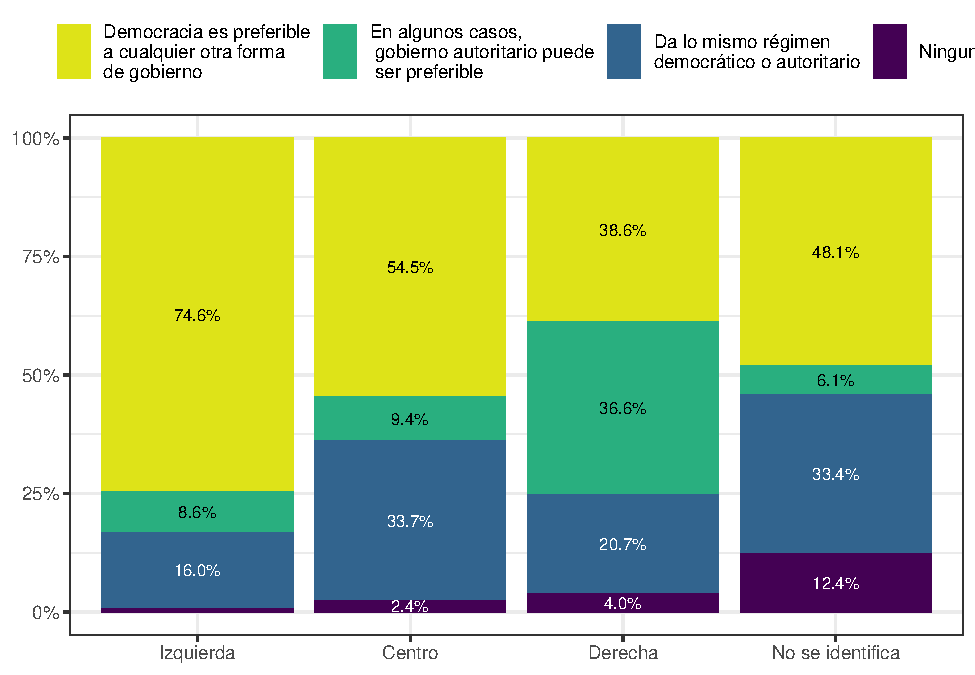
\includegraphics{reporte-elsoc_files/figure-latex/unnamed-chunk-25-1.pdf}

\hypertarget{con-cuuxe1l-de-las-siguientes-frases-estuxe1-usted-muxe1s-de-acuerdo-2021-seguxfan-posiciuxf3n-ideoluxf3gica}{%
\subsection{3.3 ¿Con cuál de las siguientes frases está usted más de acuerdo? (2021), según posición ideológica}\label{con-cuuxe1l-de-las-siguientes-frases-estuxe1-usted-muxe1s-de-acuerdo-2021-seguxfan-posiciuxf3n-ideoluxf3gica}}

\hypertarget{perfiles-ideoluxf3gicos-de-los-chilenos}{%
\chapter{Perfiles Ideológicos de los Chilenos}\label{perfiles-ideoluxf3gicos-de-los-chilenos}}

\hypertarget{clases-latentes-motivaciuxf3n}{%
\section{Clases latentes: Motivación}\label{clases-latentes-motivaciuxf3n}}

\hypertarget{bateruxeda-de-preguntas}{%
\subsection{Batería de preguntas}\label{bateruxeda-de-preguntas}}

\begin{itemize}
\tightlist
\item
  Las parejas homosexuales deberían poder adoptar hijos
\item
  El aborto debe ser legal bajo cualquier circunstancia
\item
  El Estado de Chile, más que los privados, debería ser el principal proveedor de educación
\item
  Cada persona debiera asegurarse por sí mismo su futura pensión para la tercera edad
\item
  Chile debería tomar medidas más drásticas para impedir el ingreso de inmigrantes al país
\item
  La educación sexual de los niños debería ser responsabilidad exclusiva de los padres
\item
  Se deberían clausurar empresas contaminantes, incluso si esto implica un aumento en el desempleo
\item
  El gasto social debe destinarse únicamente a los más pobres y vulnerables
\end{itemize}

\hypertarget{modelo-teuxf3rico-de-perfiles-ideuxf3logicos}{%
\section{Modelo teórico de perfiles ideólogicos}\label{modelo-teuxf3rico-de-perfiles-ideuxf3logicos}}

\hypertarget{aproximaciuxf3n-empuxedrica}{%
\subsection{Aproximación Empírica}\label{aproximaciuxf3n-empuxedrica}}

\hypertarget{perfiles-ideoluxf3gicos-resultados-principales}{%
\subsection{Perfiles ideológicos: Resultados principales}\label{perfiles-ideoluxf3gicos-resultados-principales}}

\hypertarget{justificaciuxf3n-de-la-violencia}{%
\chapter{Justificación de la Violencia}\label{justificaciuxf3n-de-la-violencia}}

\hypertarget{justificaciuxf3n-de-la-violencia-para-el-control-social-a-manos-de-ciudadanos}{%
\section{Justificación de la violencia para el control social -- a manos de ciudadanos}\label{justificaciuxf3n-de-la-violencia-para-el-control-social-a-manos-de-ciudadanos}}

\begin{verbatim}
## 2 variables were not found in the dataset: f05_01, f05_02
\end{verbatim}

\begin{figure}
\centering
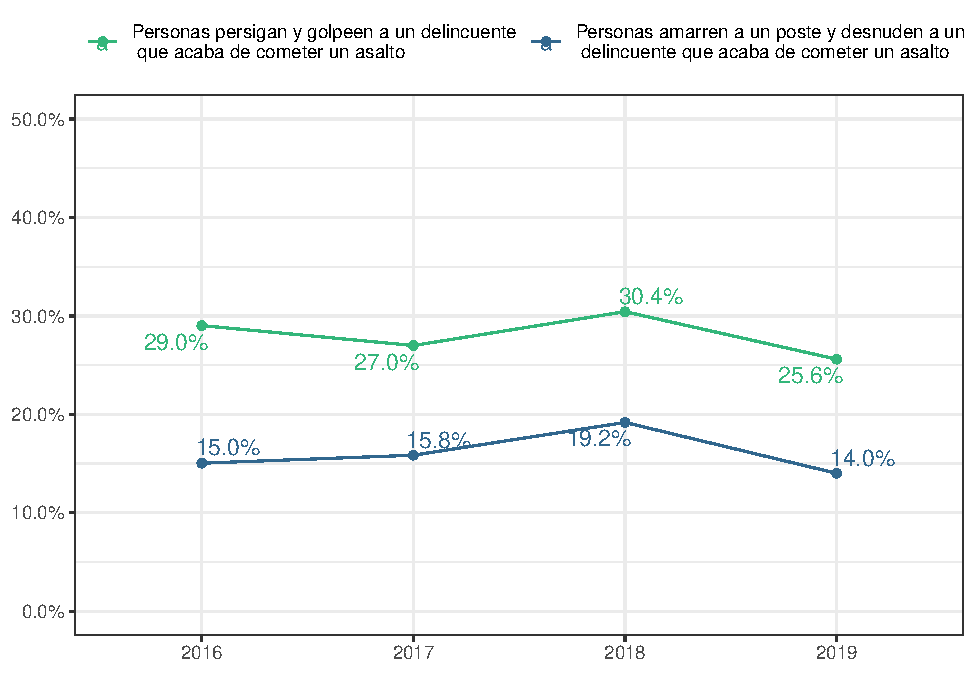
\includegraphics{reporte-elsoc_files/figure-latex/just-vio-ola-1.pdf}
\caption{\label{fig:just-vio-ola}Justificación de la violencia en relación a delincuencia, según ola de encuesta}
\end{figure}

\hypertarget{justificaciuxf3n-de-la-violencia-para-el-control-social-a-manos-de-carabineros}{%
\section{Justificación de la violencia para el control social -- a manos de carabineros}\label{justificaciuxf3n-de-la-violencia-para-el-control-social-a-manos-de-carabineros}}

\begin{verbatim}
## 3 variables were not found in the dataset: f05_03, f05_04, f05_07
\end{verbatim}

\begin{figure}

{\centering 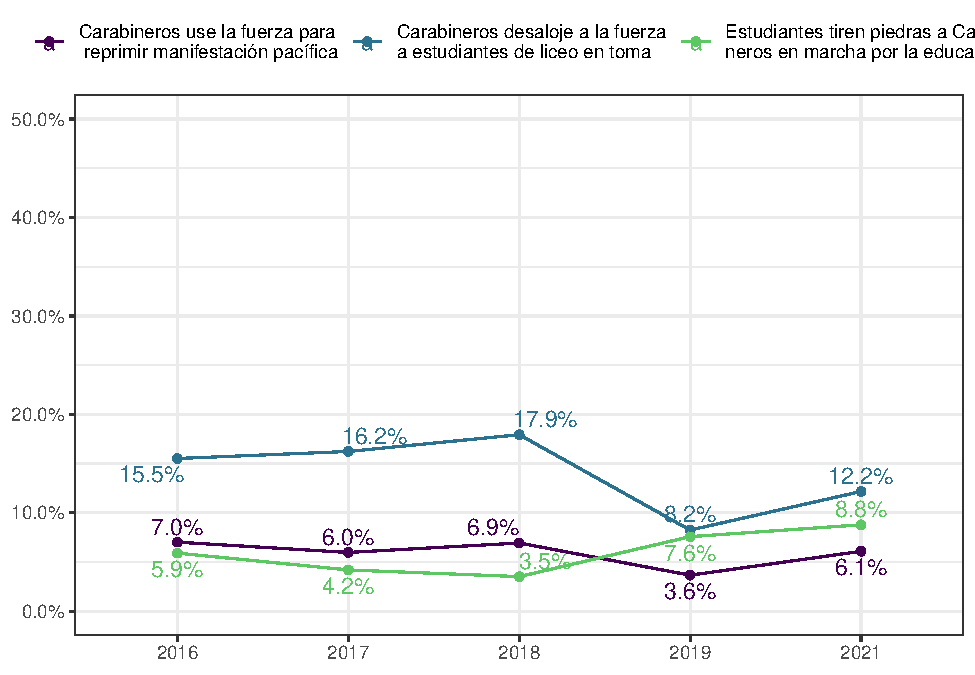
\includegraphics{reporte-elsoc_files/figure-latex/just-carab-ola-1} 

}

\caption{Justificación de la violencia en relación al actuar de Carabineros, según ola}\label{fig:just-carab-ola}
\end{figure}

\hypertarget{cambio-constitucional}{%
\chapter{Cambio Constitucional}\label{cambio-constitucional}}

\begin{figure}

{\centering 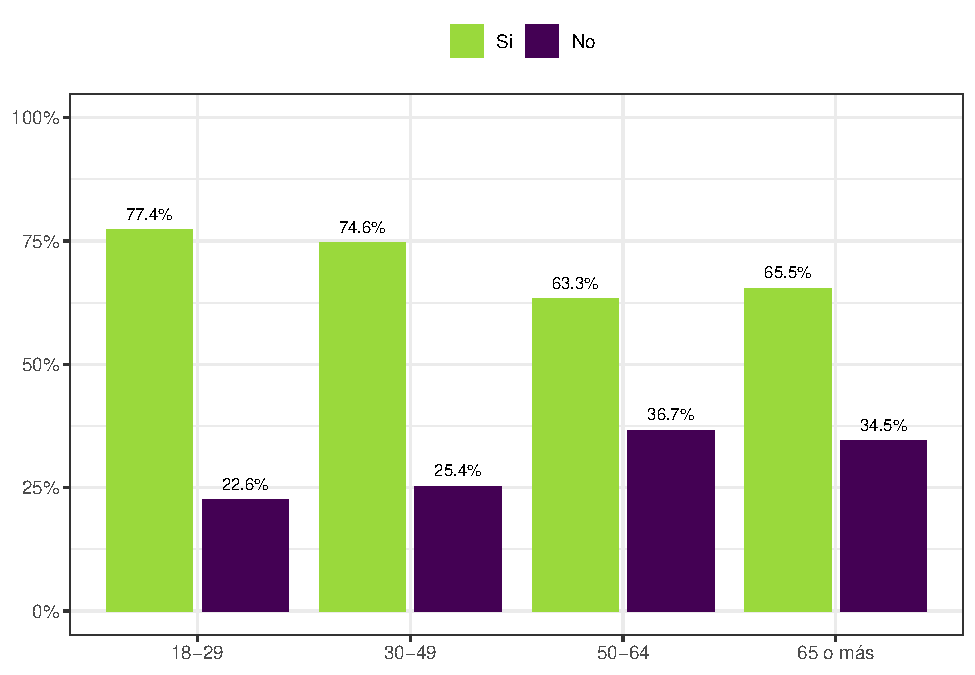
\includegraphics{reporte-elsoc_files/figure-latex/particip-edad-1} 

}

\caption{Participación en Plebiscito Nueva Constitucion}\label{fig:particip-edad}
\end{figure}

\begin{figure}

{\centering 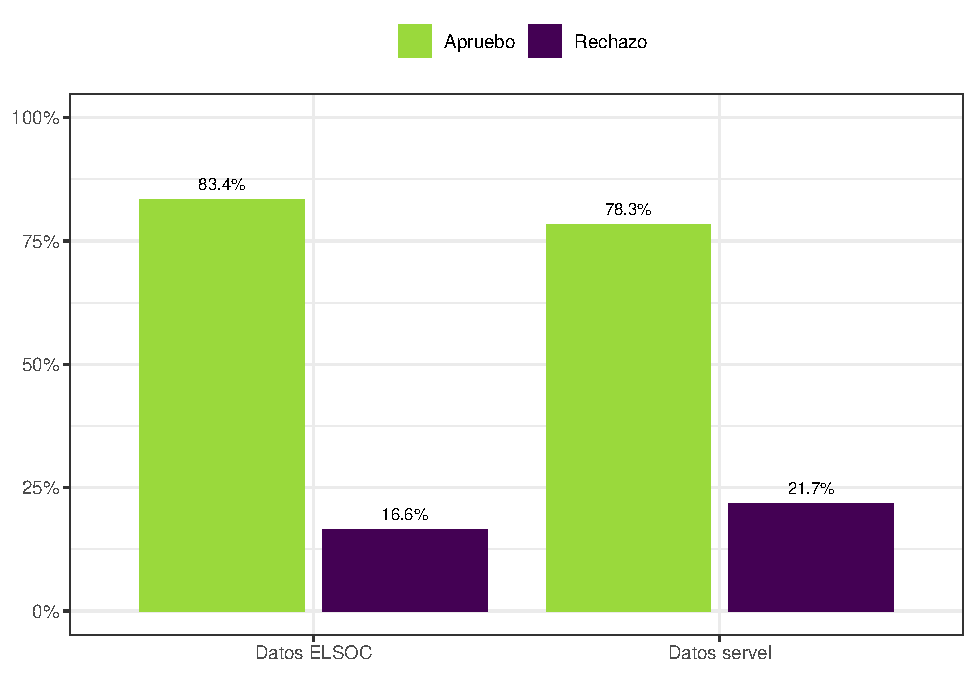
\includegraphics{reporte-elsoc_files/figure-latex/servel-apruebo-1} 

}

\caption{Voto retrospectivo Plebiscito Nueva Constitucion}\label{fig:servel-apruebo}
\end{figure}

\begin{figure}

{\centering 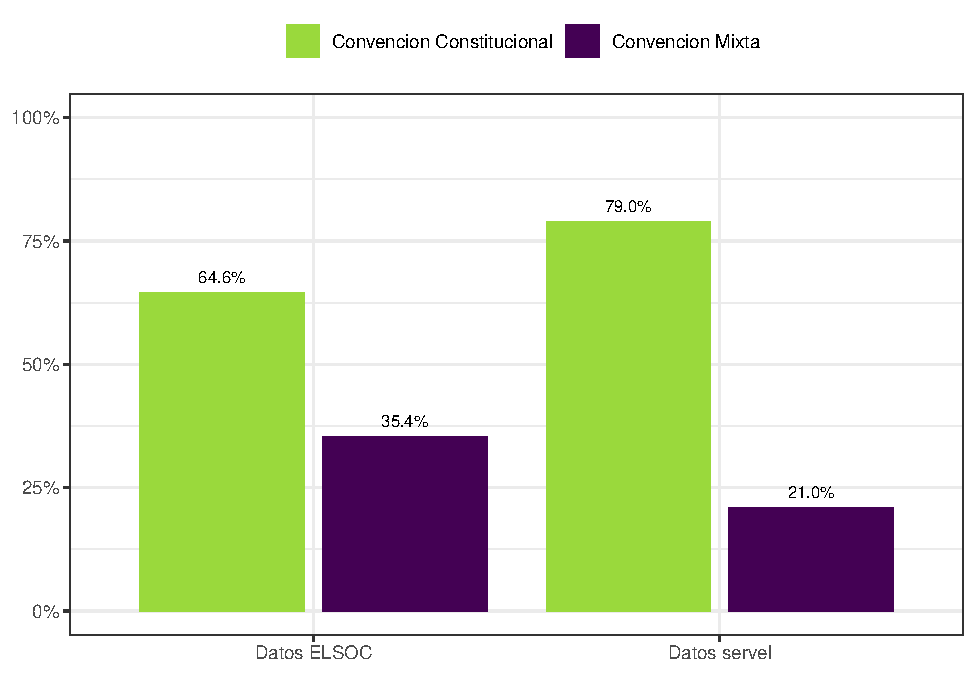
\includegraphics{reporte-elsoc_files/figure-latex/servel-cc-1} 

}

\caption{Voto Retrospectivo Plebiscito Nueva Constitucion}\label{fig:servel-cc}
\end{figure}

\begin{figure}

{\centering 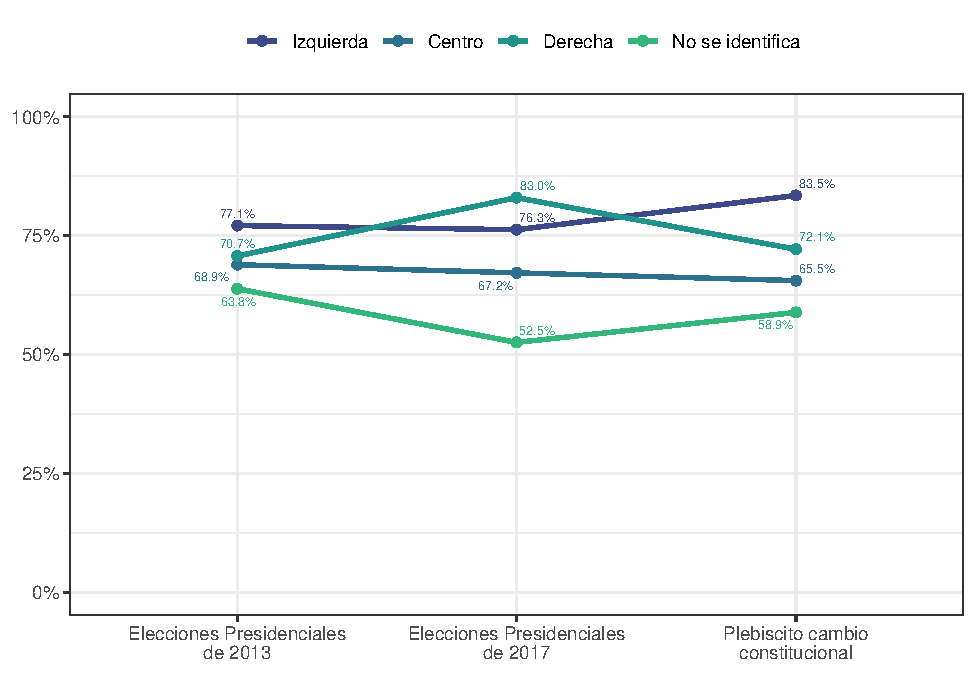
\includegraphics{reporte-elsoc_files/figure-latex/particip-elect-id-1} 

}

\caption{Sí Participa en Elecciones según Identificación Política}\label{fig:particip-elect-id}
\end{figure}

\begin{figure}

{\centering 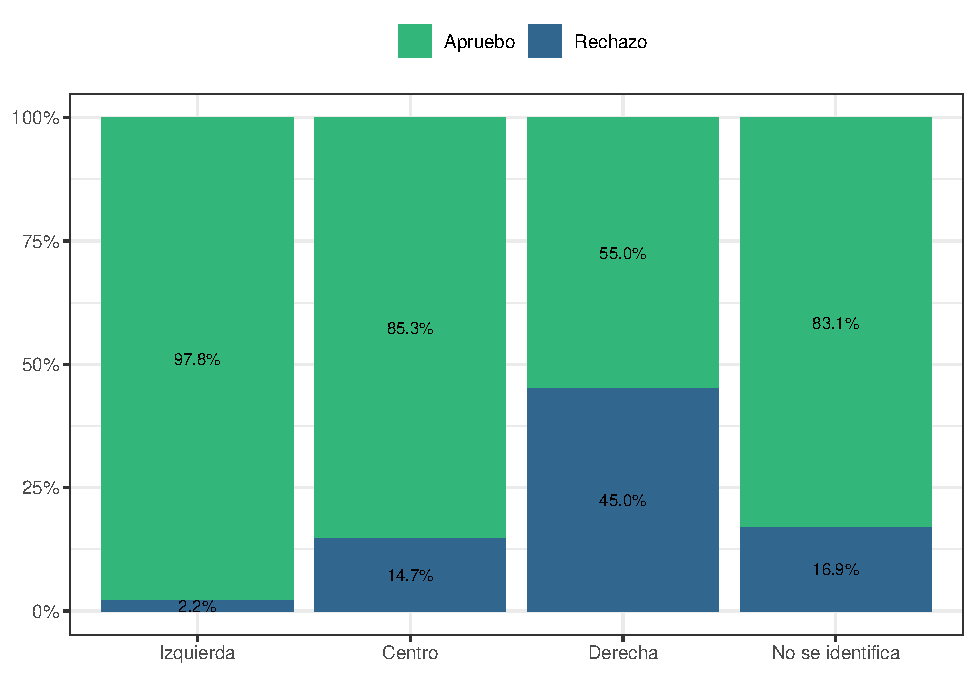
\includegraphics{reporte-elsoc_files/figure-latex/id-pol-voto-1} 

}

\caption{Voto Retrospectivo Plebicito, según Posición Ideológica}\label{fig:id-pol-voto}
\end{figure}

\hypertarget{patrones-de-votaciuxf3n}{%
\section{Patrones de Votación}\label{patrones-de-votaciuxf3n}}

\begin{figure}

{\centering 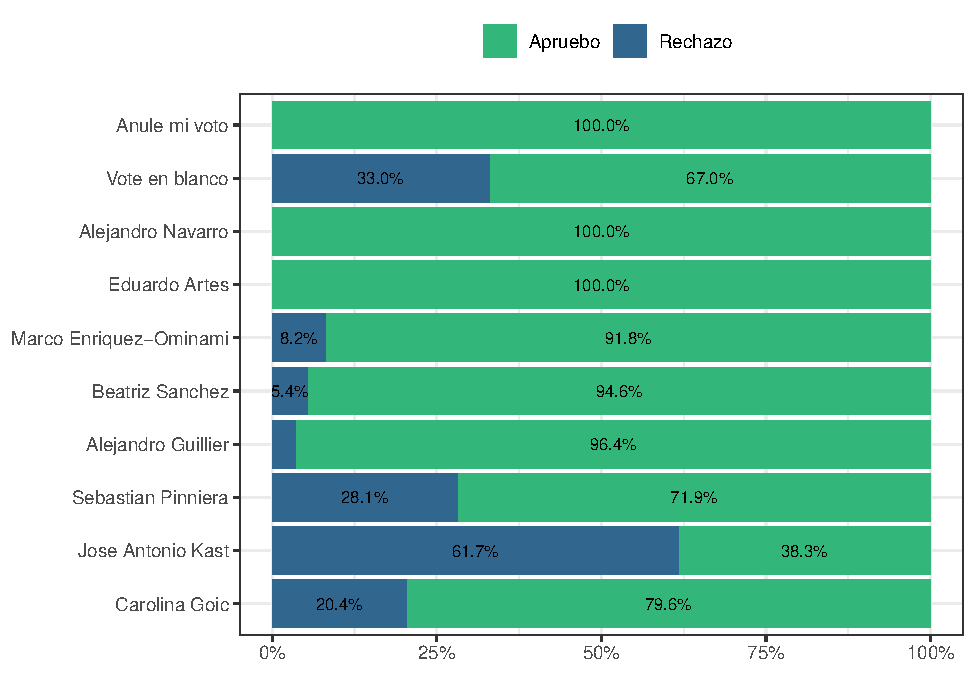
\includegraphics{reporte-elsoc_files/figure-latex/presi-voto-c44-1} 

}

\caption{Voto Retrospectivo Plebicito, según Posición Ideológica}\label{fig:presi-voto-c44}
\end{figure}

\begin{figure}

{\centering 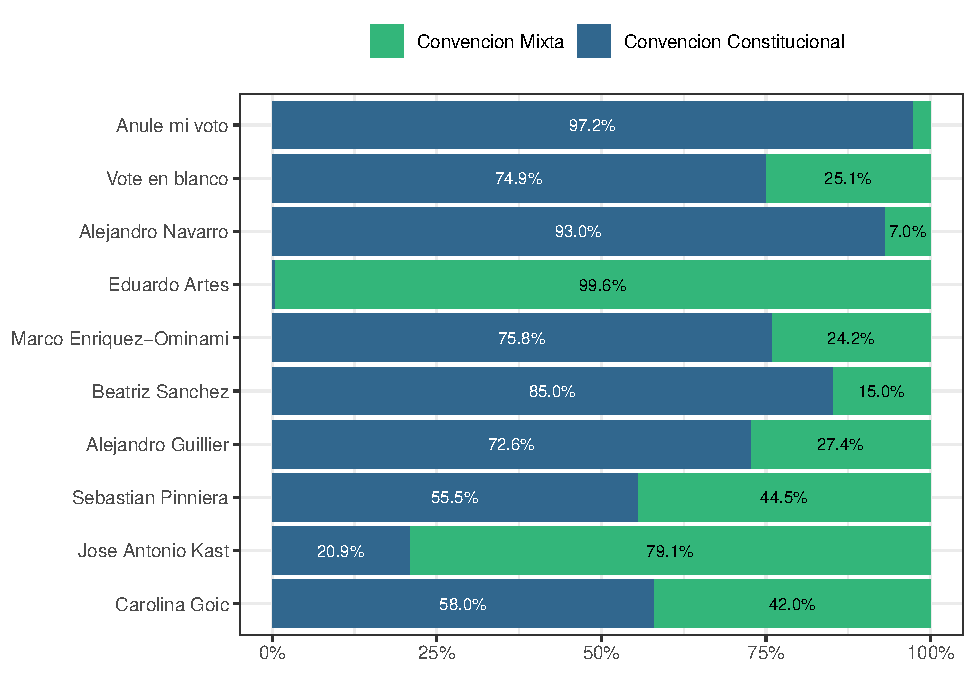
\includegraphics{reporte-elsoc_files/figure-latex/presi-voto-c45-1} 

}

\caption{Voto Retrospectivo Plebicito, según Posición Ideológica}\label{fig:presi-voto-c45}
\end{figure}

\begin{figure}

{\centering 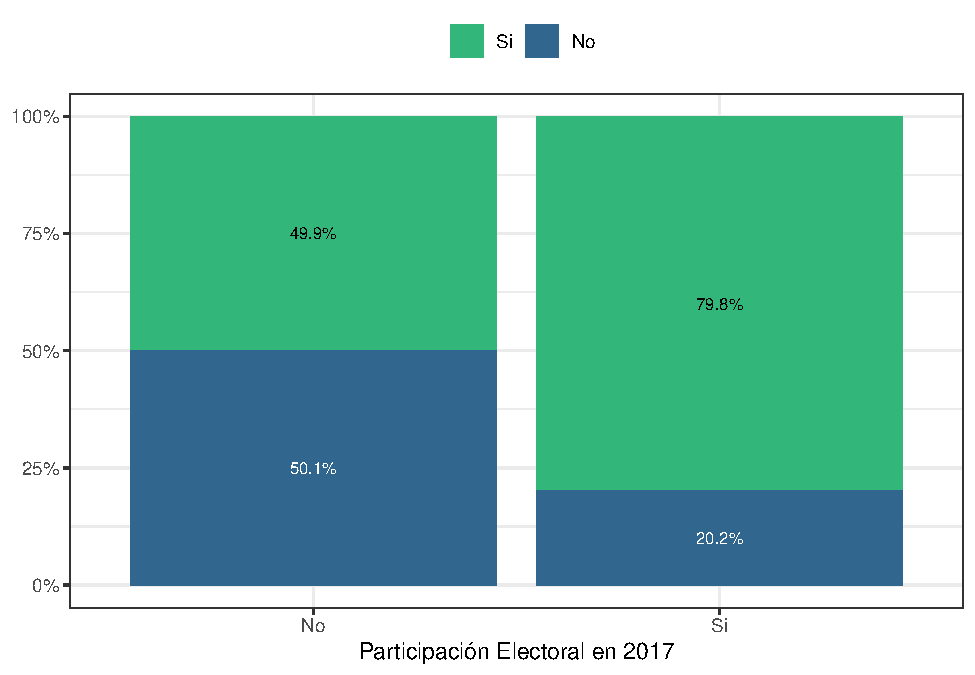
\includegraphics{reporte-elsoc_files/figure-latex/2020-vs-2021-1} 

}

\caption{Participación Electoral 2021, según la Participación en 2017}\label{fig:2020-vs-2021}
\end{figure}

\begin{verbatim}
## 
## x <categorical>
## # total N=4447  valid N=2557  mean=2.25  sd=0.91
## 
## Value                  |    N | Raw % | Valid % | Cum. %
## --------------------------------------------------------
## Se mantiene no votando |  452 | 10.16 |   17.68 |  17.68
## Cambia a votar         | 1359 | 30.56 |   53.15 |  70.83
## Cambia a No Votar      |  391 |  8.79 |   15.29 |  86.12
## Se mantiene votando    |  355 |  7.98 |   13.88 | 100.00
## <NA>                   | 1890 | 42.50 |    <NA> |   <NA>
\end{verbatim}

\hypertarget{conflicto-y-cohesiuxf3n-territorial-en-pandemia}{%
\chapter{Conflicto y cohesión territorial en pandemia}\label{conflicto-y-cohesiuxf3n-territorial-en-pandemia}}

\hypertarget{conflictividad-barrial}{%
\section{Conflictividad barrial}\label{conflictividad-barrial}}

\begin{figure}

{\centering 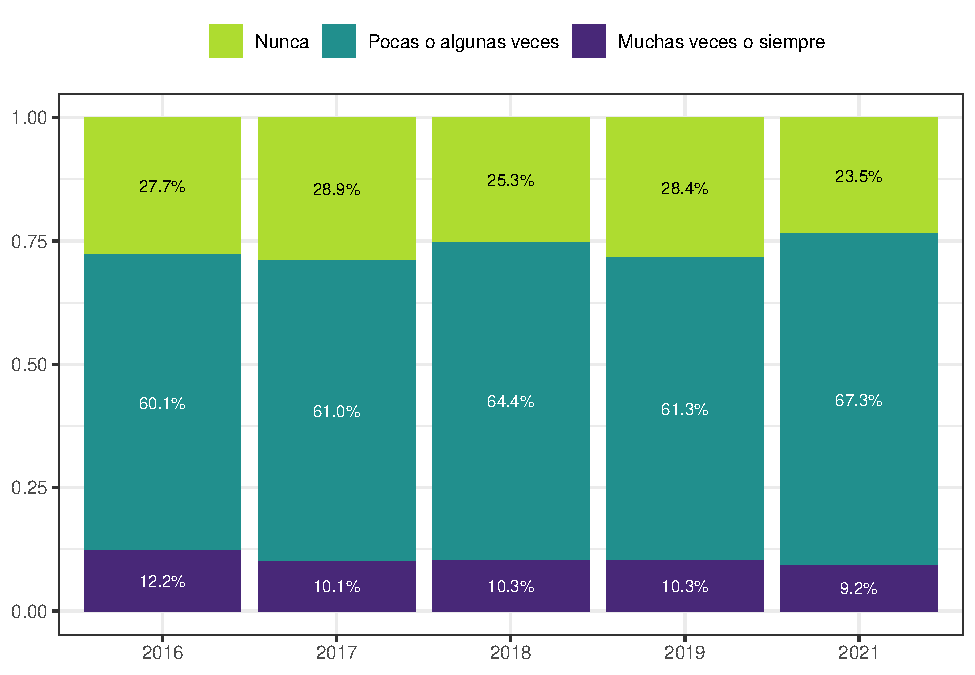
\includegraphics{reporte-elsoc_files/figure-latex/confli-olas-1} 

}

\caption{¿Con qué frecuencia usted/alguien de su hogar se ha molestado o incomodado por problemas con sus vecinos? según ola de estudio }\label{fig:confli-olas}
\end{figure}

\begin{figure}

{\centering 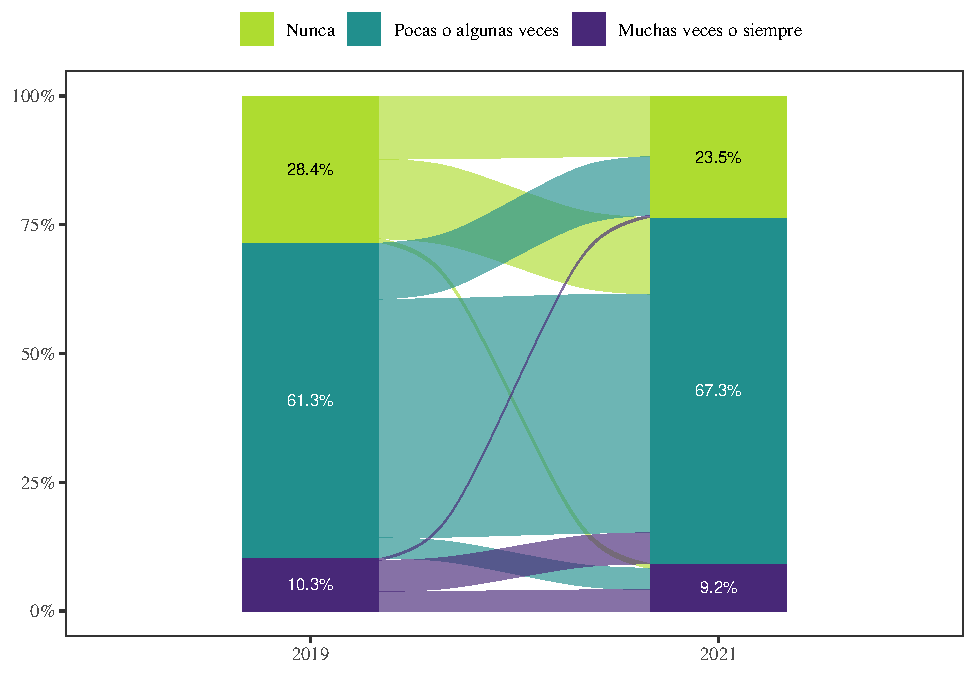
\includegraphics{reporte-elsoc_files/figure-latex/confli-cambio-1} 

}

\caption{Cambios en frecuencia de conflictos barriales}\label{fig:confli-cambio}
\end{figure}

\begin{figure}

{\centering 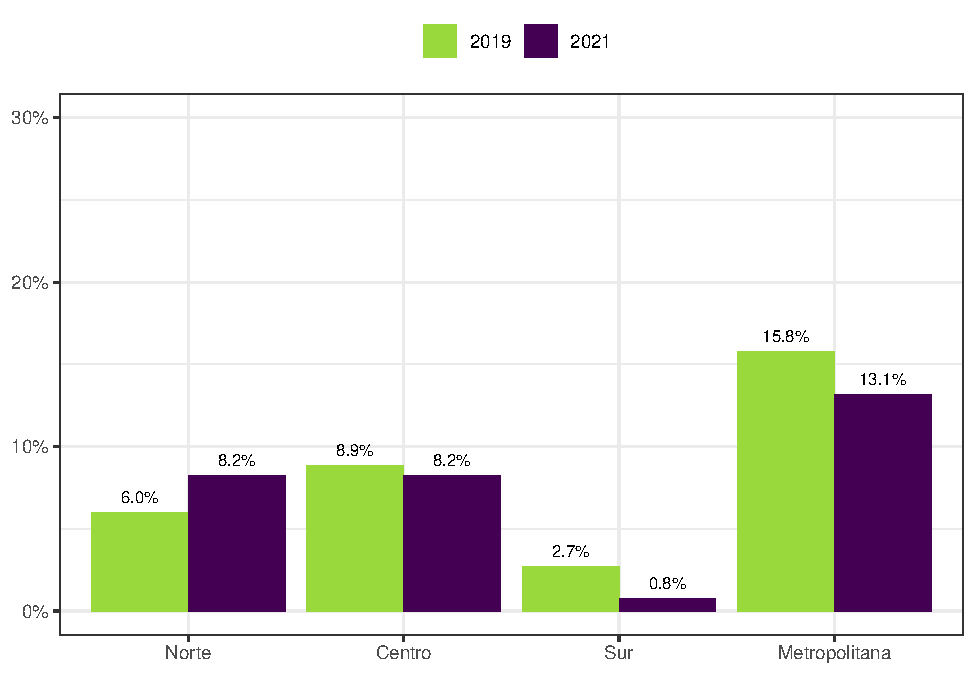
\includegraphics{reporte-elsoc_files/figure-latex/confli-zona-1} 

}

\caption{Porcentaje con alta frecuencia de conflictos barriales, según ola del estudio y zona geográfica. Porcentaje con conflictos barriales "Siempre" o "Muchas veces"}\label{fig:confli-zona}
\end{figure}

\begin{figure}

{\centering 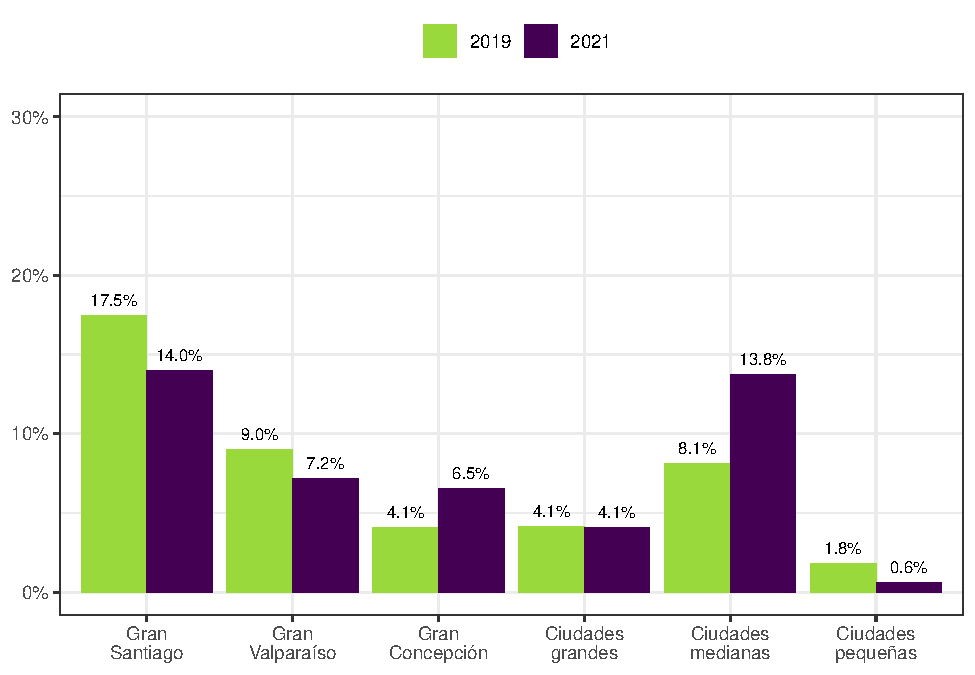
\includegraphics{reporte-elsoc_files/figure-latex/confli-estrato-1} 

}

\caption{Porcentaje con alta frecuencia de conflictos barriales, según ola del estudio y zona de residencia. Porcentaje con conflictos barriales "Siempre" o "Muchas veces".}\label{fig:confli-estrato}
\end{figure}

\begin{figure}

{\centering 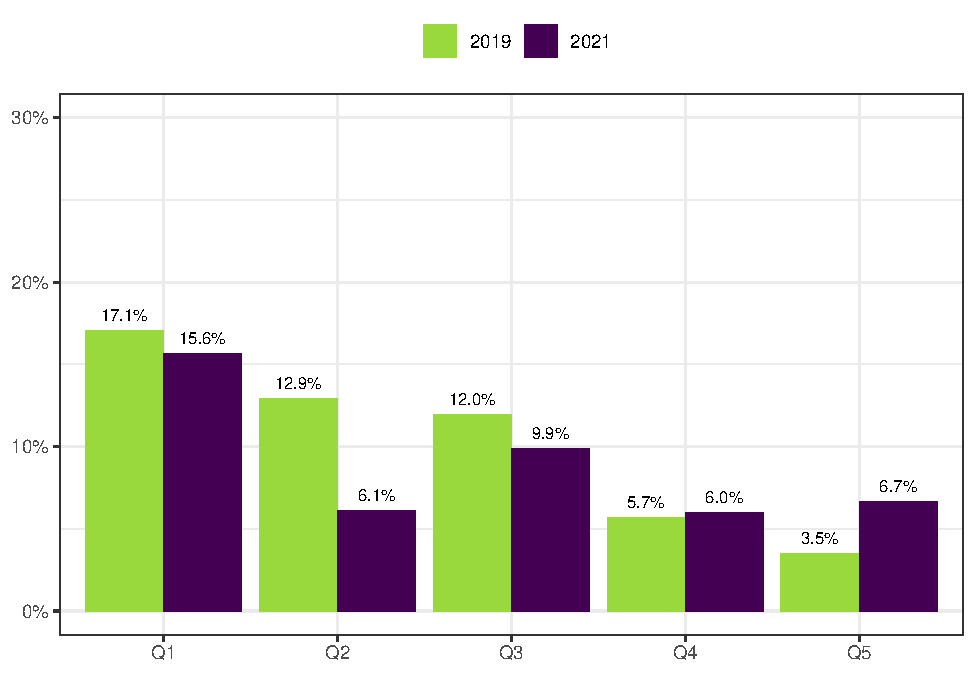
\includegraphics{reporte-elsoc_files/figure-latex/confli-quintil-1} 

}

\caption{Porcentaje con alta frecuencia de conflictos barriales, según ola del estudio y quintil de ingreso. Porcentaje con conflictos barriales "Siempre" o "Muchas veces".}\label{fig:confli-quintil}
\end{figure}

\hypertarget{cartografuxeda-del-conflicto-barrial}{%
\subsection{Cartografía del conflicto barrial}\label{cartografuxeda-del-conflicto-barrial}}

\begin{figure}

{\centering 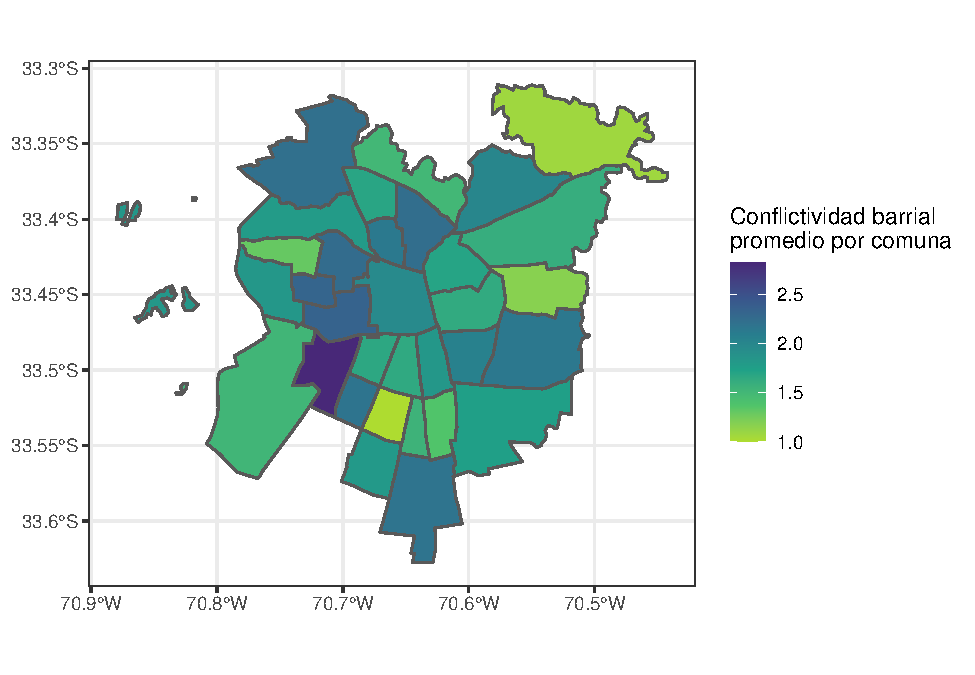
\includegraphics{reporte-elsoc_files/figure-latex/confli-comuna-1} 

}

\caption{Frecuencia promedio de problemas con vecinos, según comuna de residencia en la región metropolitana (2021).}\label{fig:confli-comuna}
\end{figure}

\begin{figure}

{\centering 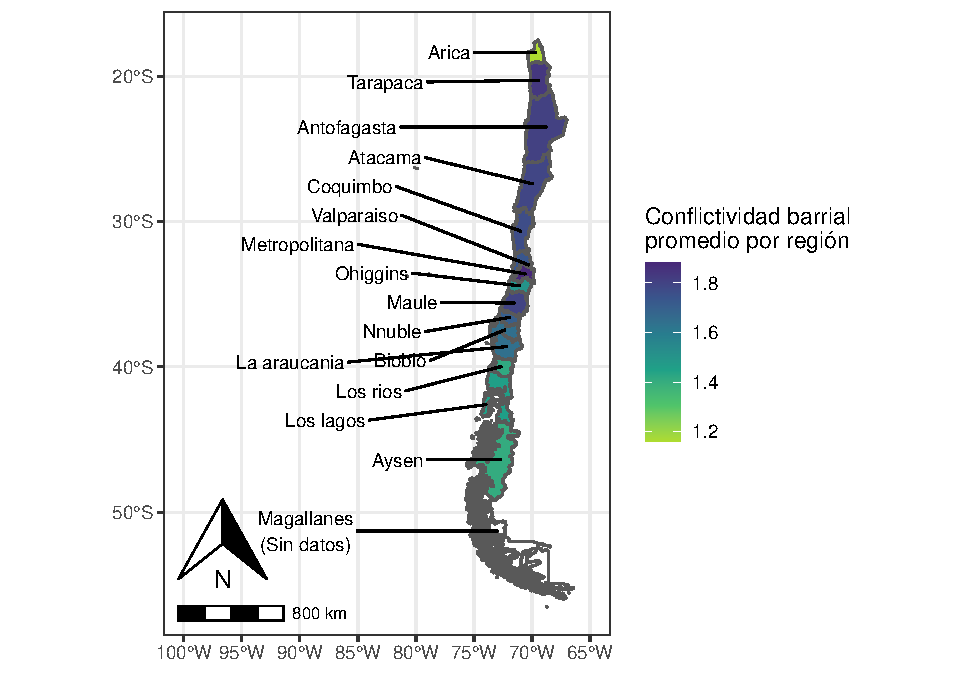
\includegraphics{reporte-elsoc_files/figure-latex/confli-region2-1} 

}

\caption{Frecuencia promedio de problemas con vecinos, según región de Chile (2021)}\label{fig:confli-region2}
\end{figure}

\hypertarget{confianza-en-vecinos}{%
\section{Confianza en vecinos}\label{confianza-en-vecinos}}

\begin{figure}

{\centering 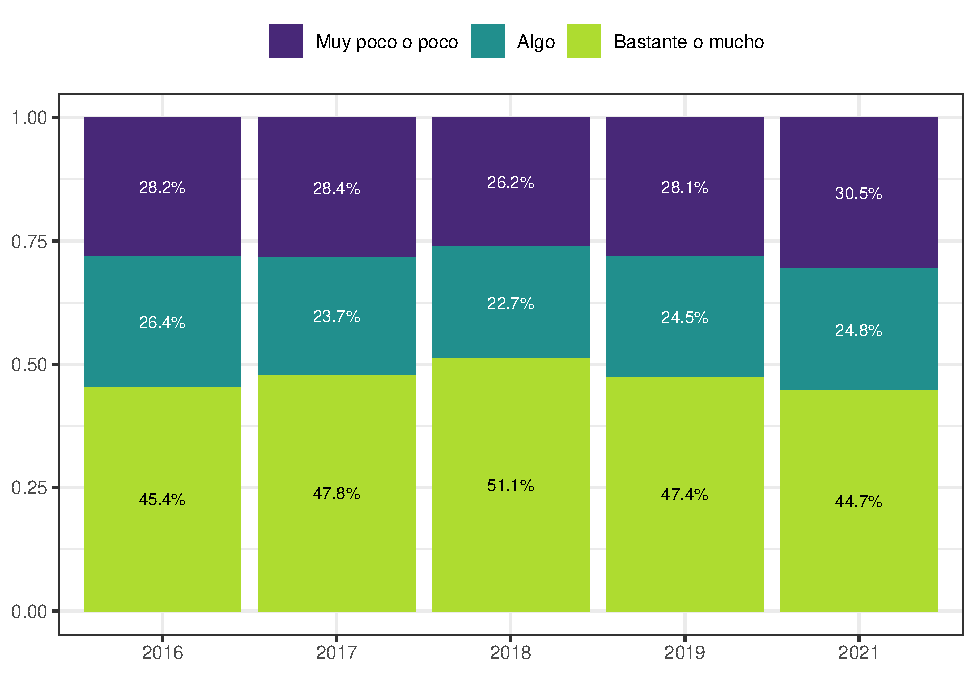
\includegraphics{reporte-elsoc_files/figure-latex/vecinos-ola-1} 

}

\caption{En términos generales, ¿cuánto confía usted en sus vecinos? según ola de estudio.}\label{fig:vecinos-ola}
\end{figure}

\begin{figure}

{\centering 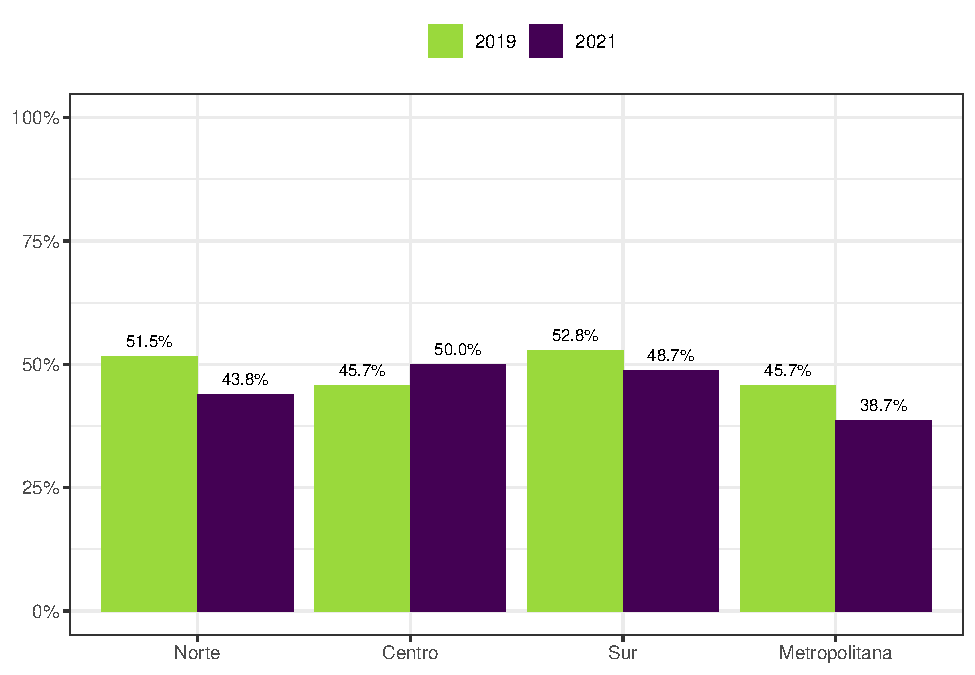
\includegraphics{reporte-elsoc_files/figure-latex/vecinos-zona-1} 

}

\caption{En términos generales, ¿cuánto confía usted en sus vecinos? Según ola del estudio y zona geográfica. Suma de Respuestas “Bastante” y “Mucho”.}\label{fig:vecinos-zona}
\end{figure}

\begin{figure}

{\centering 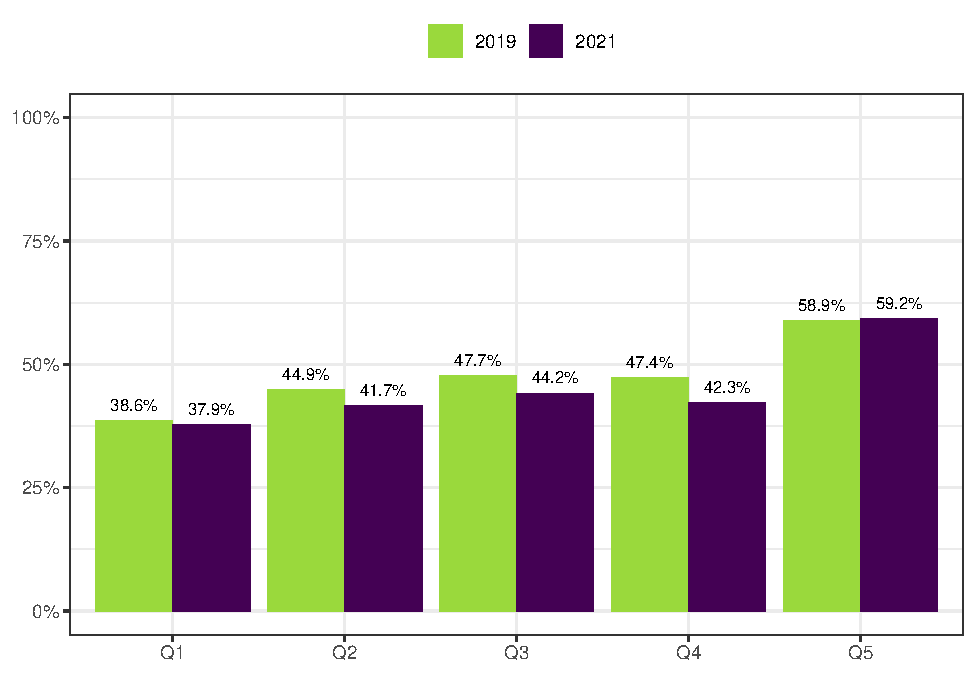
\includegraphics{reporte-elsoc_files/figure-latex/vecinos-quintil-1} 

}

\caption{En términos generales, ¿cuánto confía usted en sus vecinos? Según ola del estudio y quintil de ingreso. Suma de Respuestas “Bastante” y “Mucho”.}\label{fig:vecinos-quintil}
\end{figure}

\hypertarget{seguridad-barrial}{%
\section{Seguridad barrial}\label{seguridad-barrial}}

\begin{figure}

{\centering 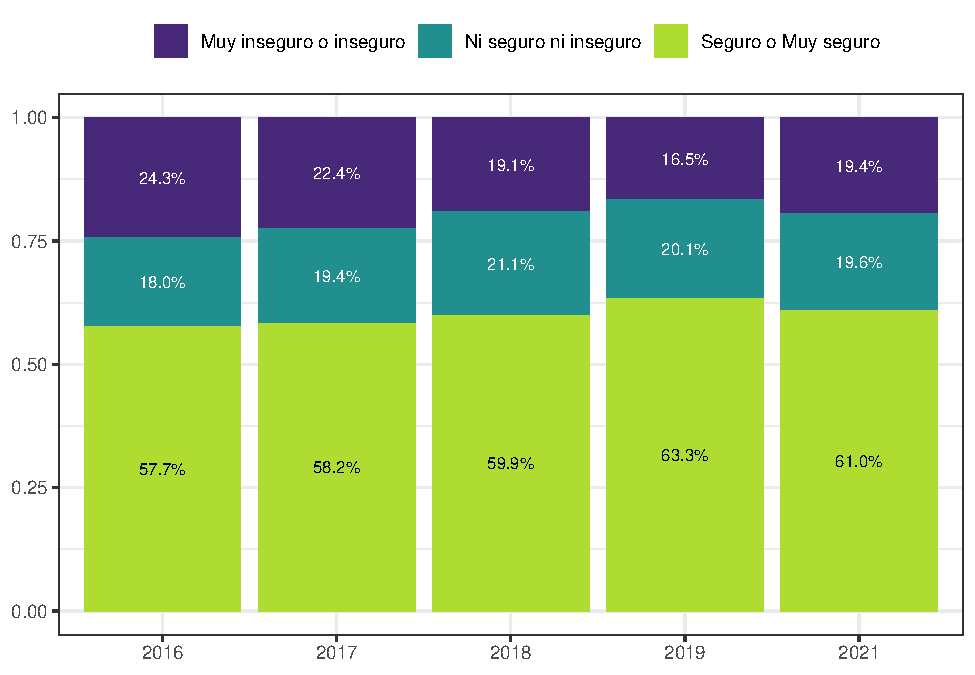
\includegraphics{reporte-elsoc_files/figure-latex/seguri-ola-1} 

}

\caption{¿Qué tan seguro o inseguro se siente en el barrio o vecindario donde usted vive? Según ola del estudio.}\label{fig:seguri-ola}
\end{figure}

\begin{figure}

{\centering 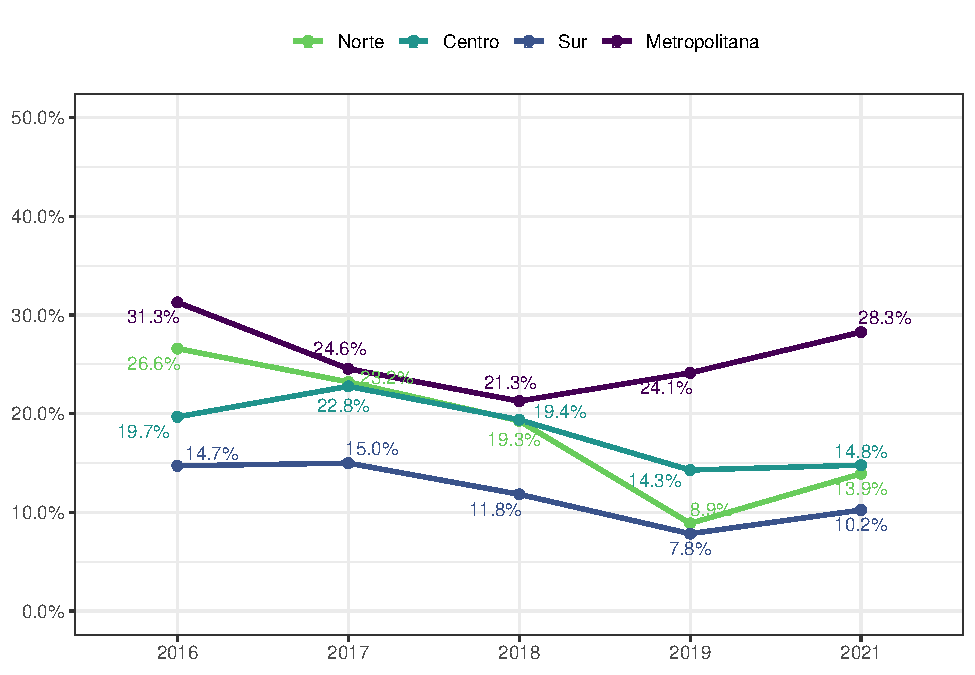
\includegraphics{reporte-elsoc_files/figure-latex/seguri-zona-1} 

}

\caption{¿Qué tan seguro o inseguro se siente en el barrio o vecindario donde usted vive? Según ola del estudio y zona geográfica. Suma de Respuestas "Inseguro" o ”Muy Inseguro".}\label{fig:seguri-zona}
\end{figure}

\begin{figure}

{\centering 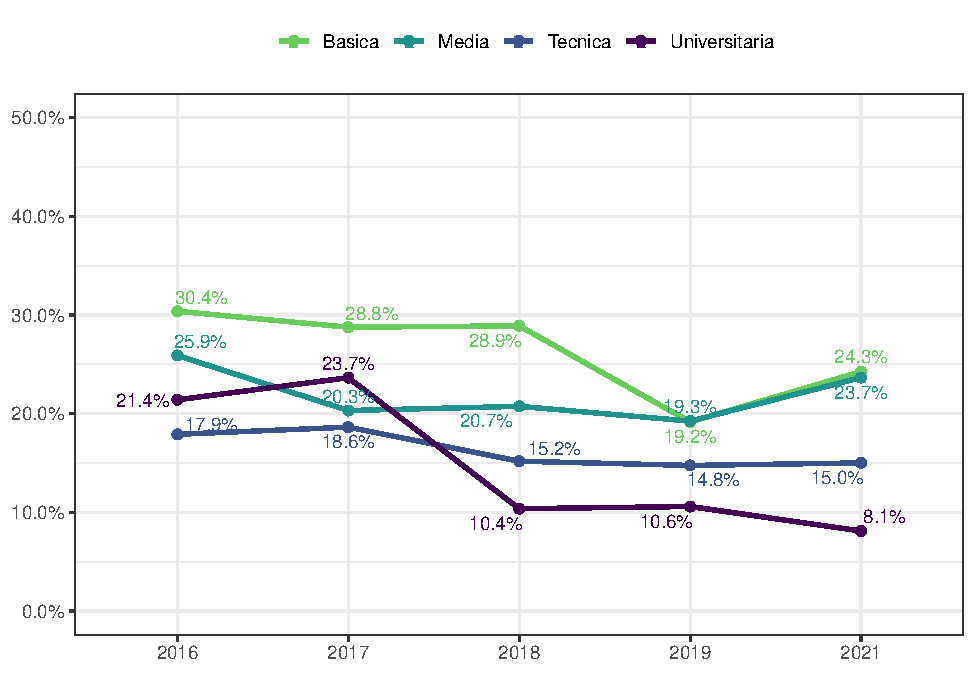
\includegraphics{reporte-elsoc_files/figure-latex/seguri-educ-1} 

}

\caption{¿Qué tan seguro o inseguro se siente en el barrio o vecindario donde usted vive? Según ola del estudio y nivel educacional. Suma de Respuestas "Inseguro" o ”Muy Inseguro".}\label{fig:seguri-educ}
\end{figure}

\begin{figure}

{\centering 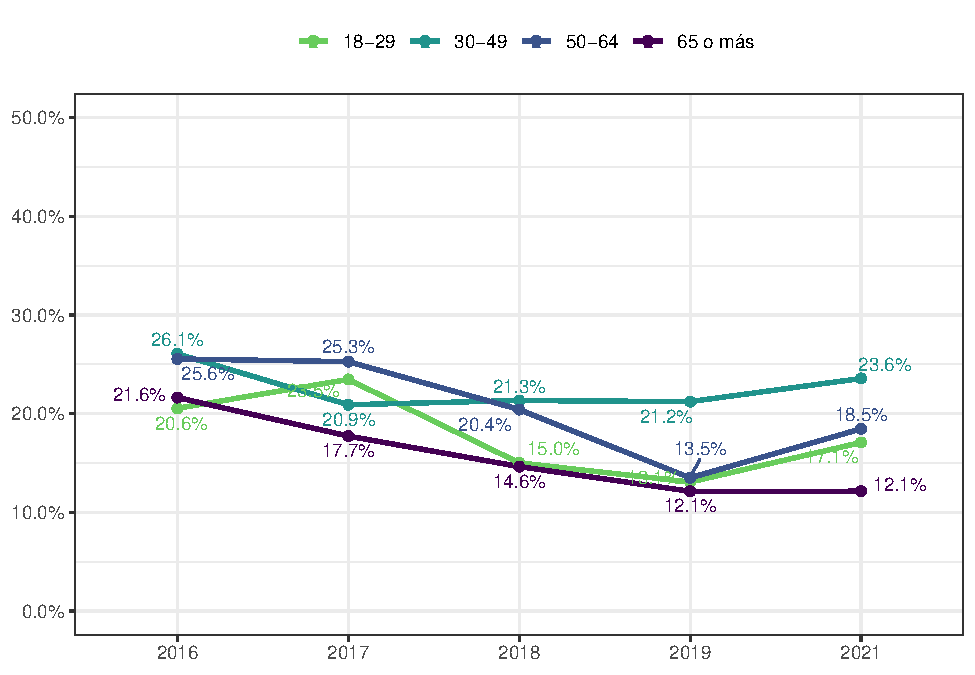
\includegraphics{reporte-elsoc_files/figure-latex/seguri-edad-1} 

}

\caption{¿Qué tan seguro o inseguro se siente en el barrio o vecindario donde usted vive? Según ola del estudio y tramos de edad. Suma de Respuestas "Inseguro" o ”Muy Inseguro".}\label{fig:seguri-edad}
\end{figure}

\begin{figure}

{\centering 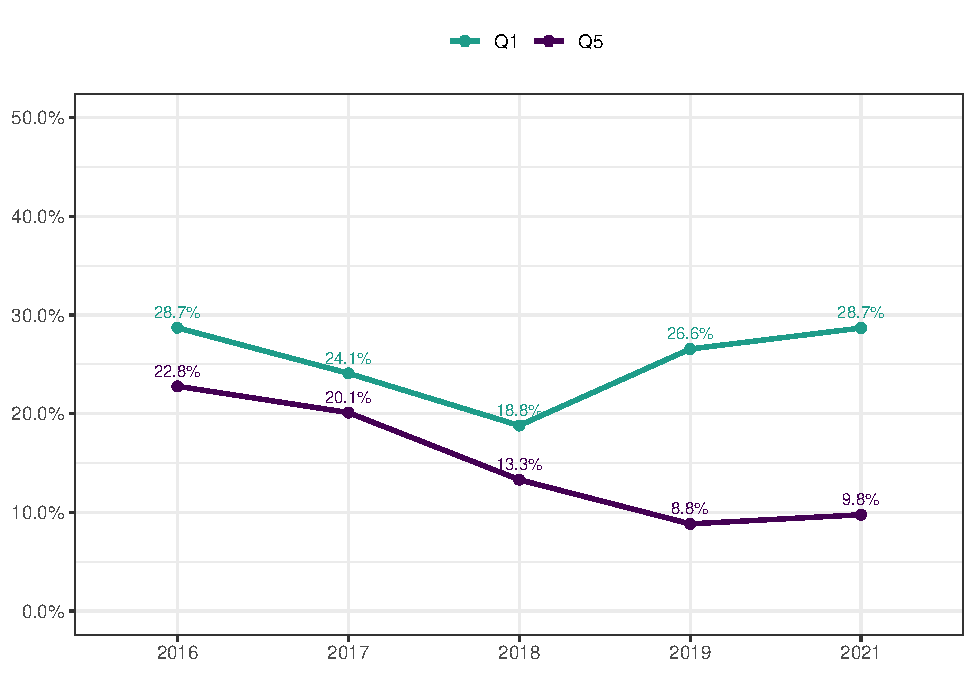
\includegraphics{reporte-elsoc_files/figure-latex/seguri-quintil-1} 

}

\caption{¿Qué tan seguro o inseguro se siente en el barrio o vecindario donde usted vive? Según ola del estudio y quintil de ingreso per capita. Suma de Respuestas "Seguro" o ”Muy Seguro".}\label{fig:seguri-quintil}
\end{figure}

\hypertarget{criminalidad-barrial}{%
\section{Criminalidad barrial}\label{criminalidad-barrial}}

\begin{figure}

{\centering 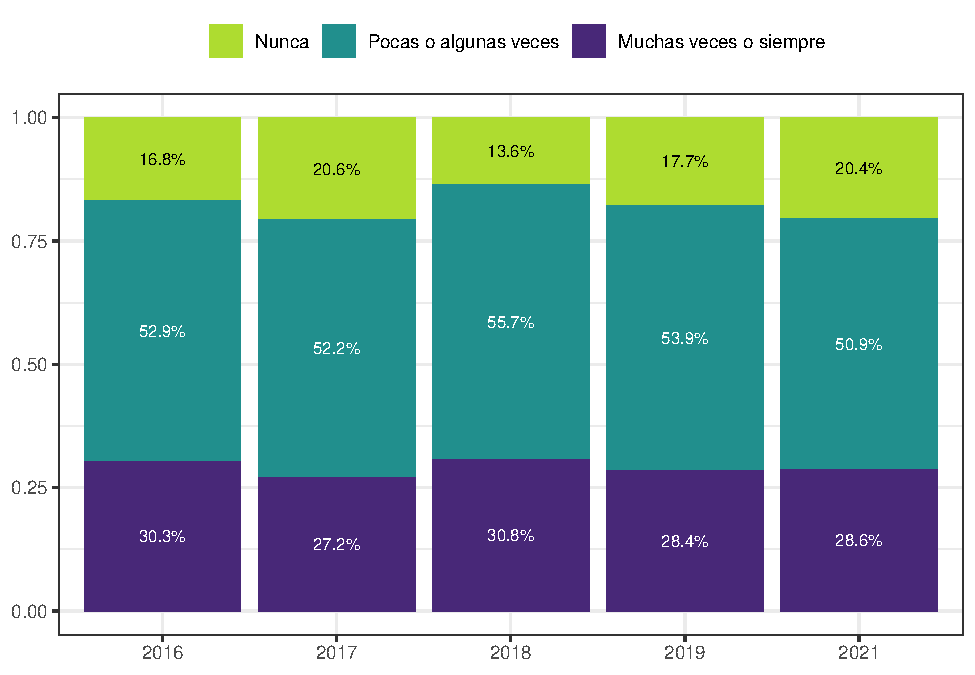
\includegraphics{reporte-elsoc_files/figure-latex/crim-olas-1} 

}

\caption{¿Con qué frecuencia se han producido crímenes (riñas, robos y tráfico de drogas) en su barrio?, según ola de estudio.}\label{fig:crim-olas}
\end{figure}

\begin{figure}

{\centering 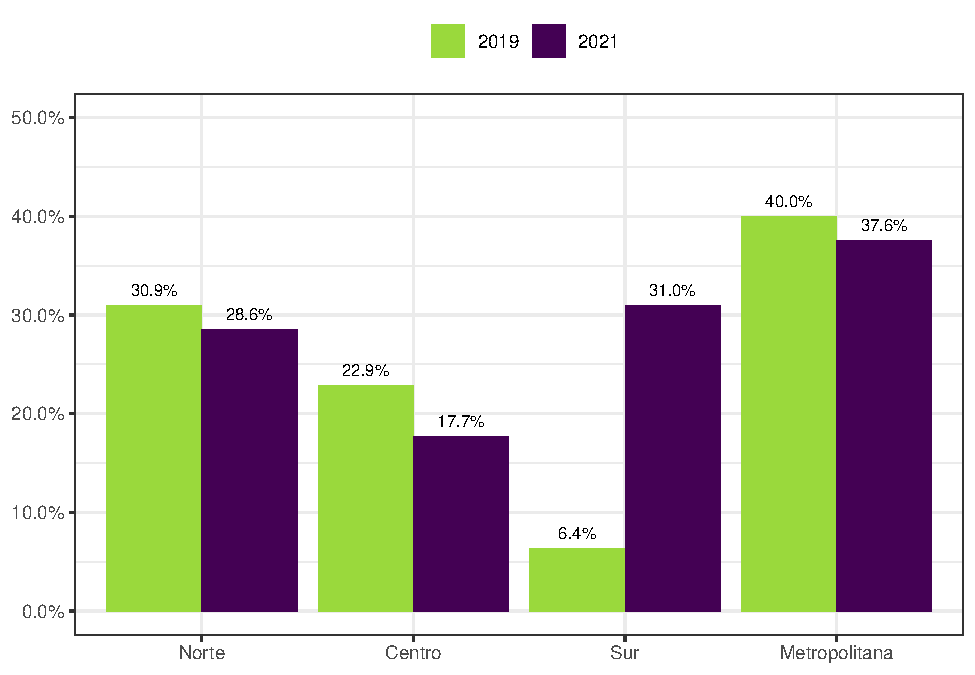
\includegraphics{reporte-elsoc_files/figure-latex/crim-zona-1} 

}

\caption{¿Con qué frecuencia se han producido crímenes (riñas, robos y tráfico de drogas) en su barrio?, según ola del estudio y zona geográfica. Porcentaje de experiencias de criminalidad "Siempre" o "Muchas veces".}\label{fig:crim-zona}
\end{figure}

\begin{figure}

{\centering 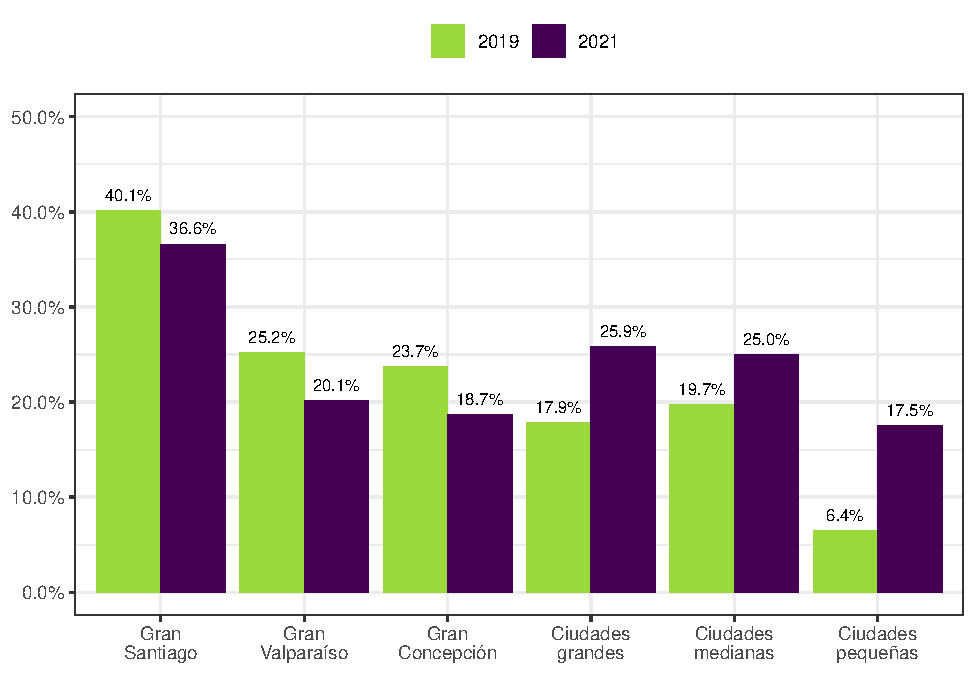
\includegraphics{reporte-elsoc_files/figure-latex/crim-estrato-1} 

}

\caption{¿Con qué frecuencia se han producido crímenes (riñas, robos y tráfico de drogas) en su barrio?, según ola del estudio y tipo de ciudad. Porcentaje de experiencias de criminalidad "Siempre" o "Muchas veces".}\label{fig:crim-estrato}
\end{figure}

\begin{figure}

{\centering 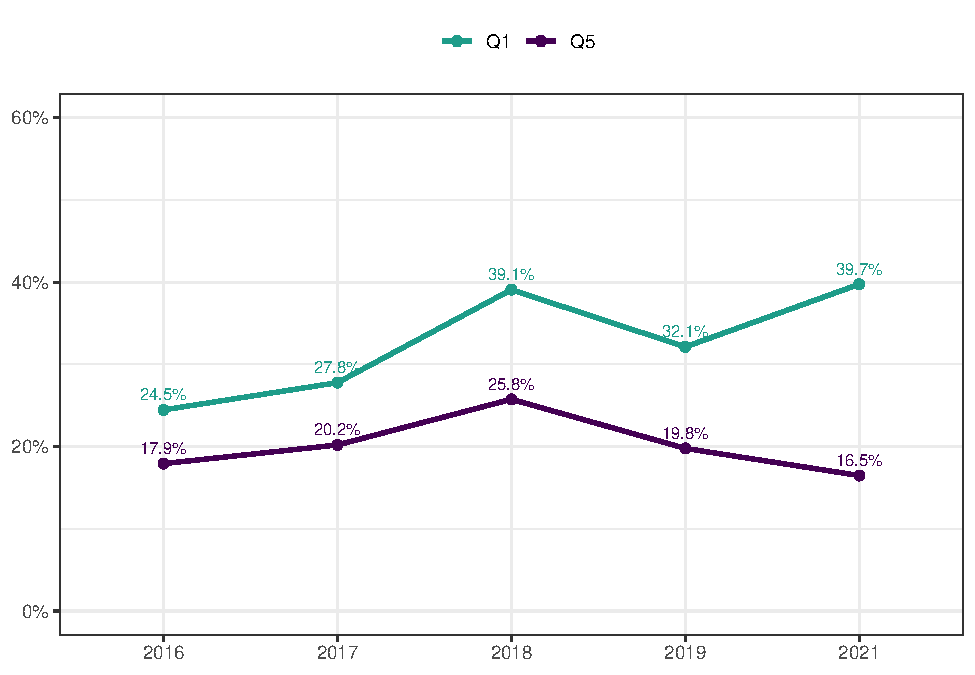
\includegraphics{reporte-elsoc_files/figure-latex/crim-quintil-1} 

}

\caption{¿Con qué frecuencia se han producido crímenes (riñas, robos y tráfico de drogas) en su barrio?, según ola del estudio y quintil de ingreso. Porcentaje de experiencias de criminalidad "Siempre" o "Muchas veces".}\label{fig:crim-quintil}
\end{figure}

\hypertarget{cartografuxeda-de-la-criminalidad-barrial}{%
\subsection{Cartografía de la criminalidad barrial}\label{cartografuxeda-de-la-criminalidad-barrial}}

\begin{figure}

{\centering 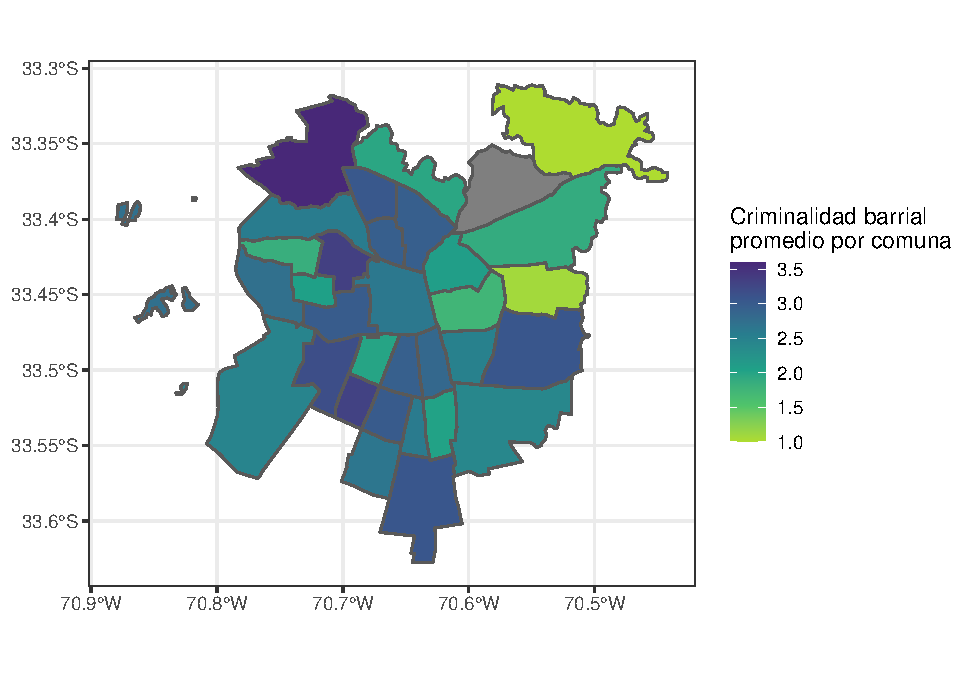
\includegraphics{reporte-elsoc_files/figure-latex/crimi-comuna-1} 

}

\caption{Frecuencia promedio de percepción de crímenes (riñas, robos y tráfico de drogas) en el barrio, según comuna de residencia en la región metropolitana (2021).}\label{fig:crimi-comuna}
\end{figure}

\begin{figure}

{\centering 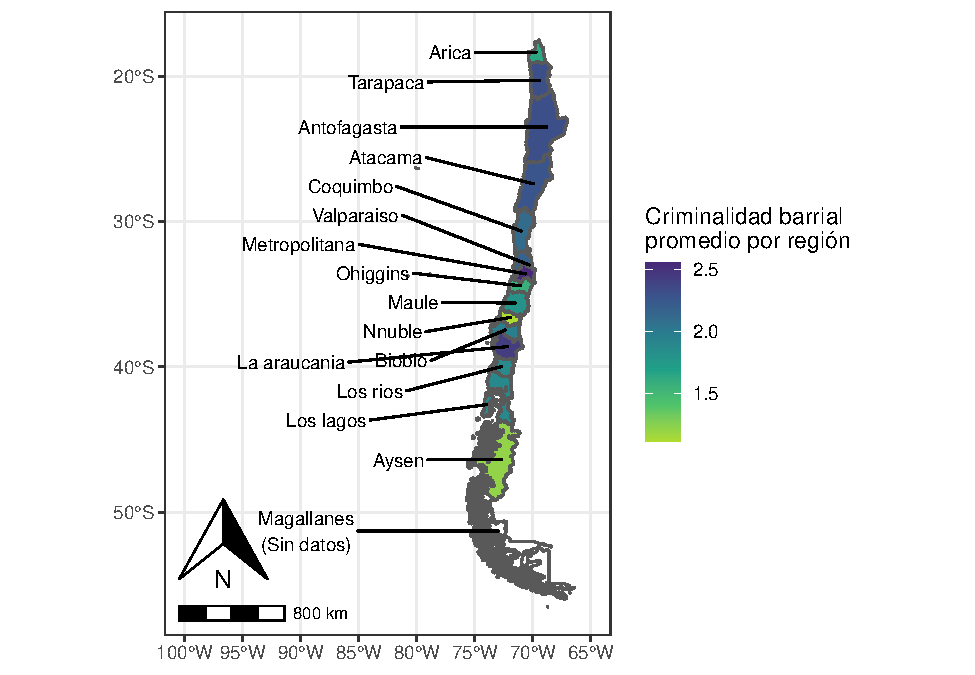
\includegraphics{reporte-elsoc_files/figure-latex/confli-region-1} 

}

\caption{Frecuencia promedio de percepción de crímenes (riñas, robos y tráfico de drogas) en el barrio, según región de Chile (2021)}\label{fig:confli-region}
\end{figure}

\hypertarget{distanciamiento-y-comportamiento-prosocial-en-pandemia}{%
\chapter{Distanciamiento y comportamiento prosocial en pandemia}\label{distanciamiento-y-comportamiento-prosocial-en-pandemia}}

\hypertarget{distanciamiento-social}{%
\section{Distanciamiento social}\label{distanciamiento-social}}

\begin{figure}

{\centering 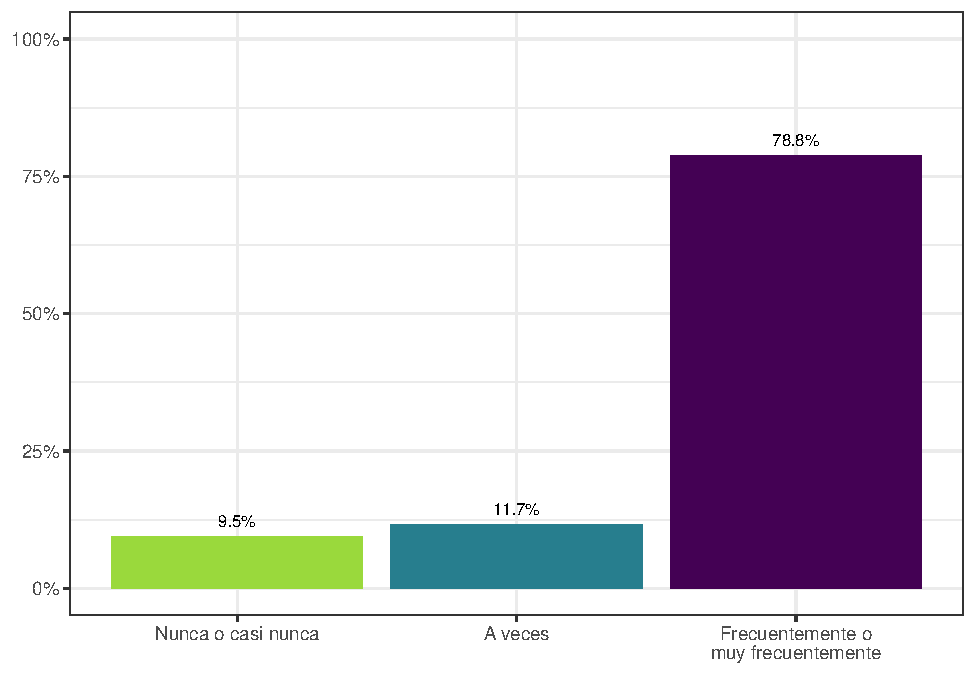
\includegraphics{reporte-elsoc_files/figure-latex/dist-total-1} 

}

\caption{¿En qué medida usted ha seguido la recomendación de quedarse en su hogar, manteniendo el aislamiento social? (2021).}\label{fig:dist-total}
\end{figure}

\begin{figure}

{\centering 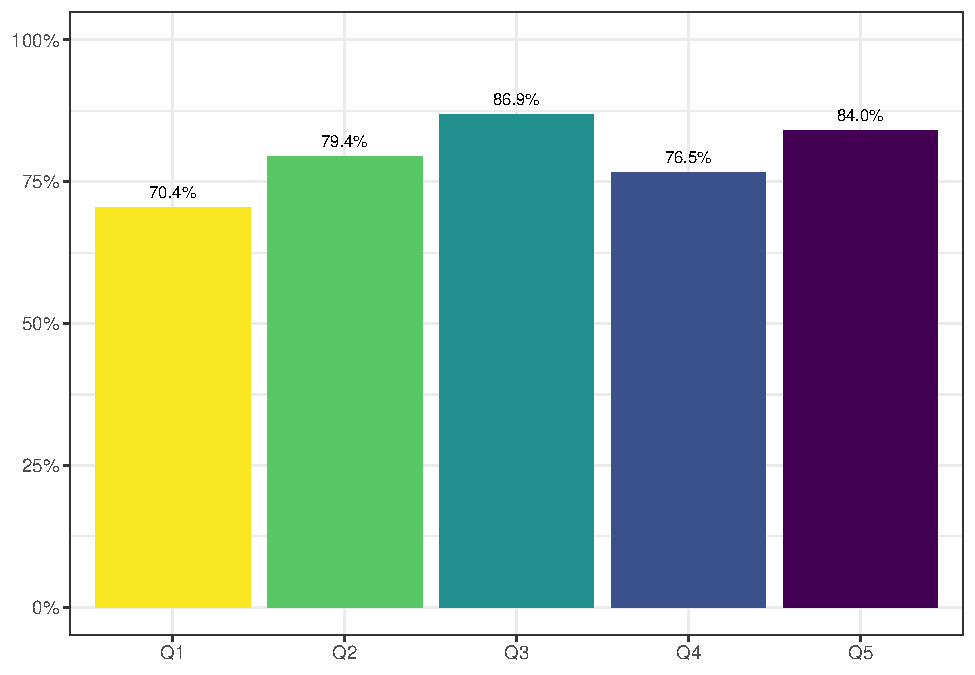
\includegraphics{reporte-elsoc_files/figure-latex/dist-quintil-1} 

}

\caption{¿En qué medida usted ha seguido la recomendación de quedarse en su hogar, manteniendo el aislamiento social? según quintil de ingreso. Suma de respuestas "Frecuente o "Muy frecuentemente" (2021).}\label{fig:dist-quintil}
\end{figure}

\begin{figure}

{\centering 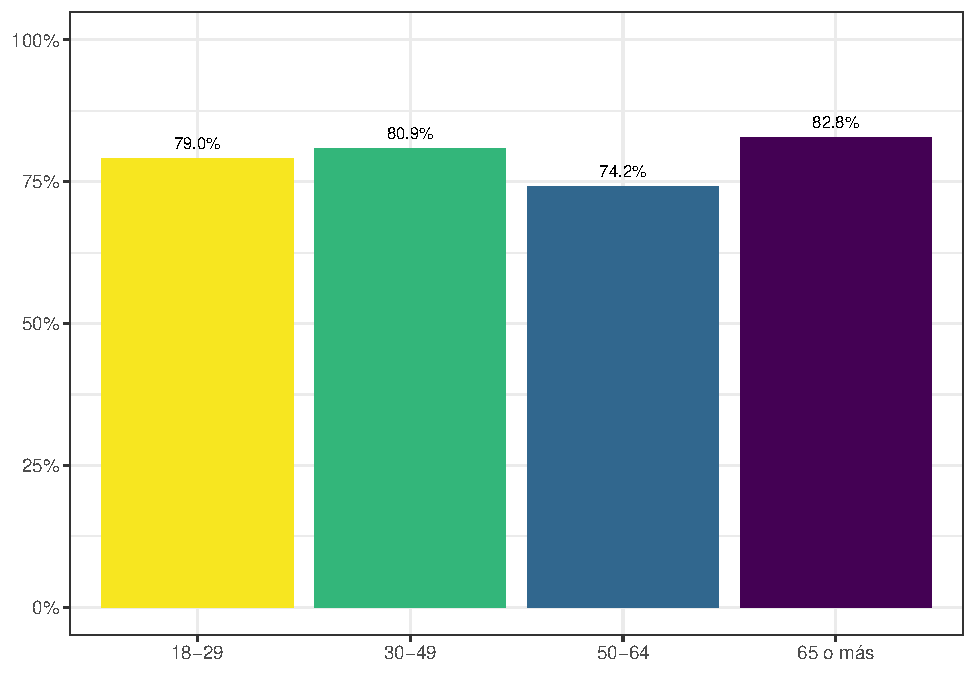
\includegraphics{reporte-elsoc_files/figure-latex/dist-edad-1} 

}

\caption{¿En qué medida usted ha seguido la recomendación de quedarse en su hogar, manteniendo el aislamiento social? según edad. Suma de respuestas "Frecuente o "Muy frecuentemente" (2021).}\label{fig:dist-edad}
\end{figure}

\begin{figure}

{\centering 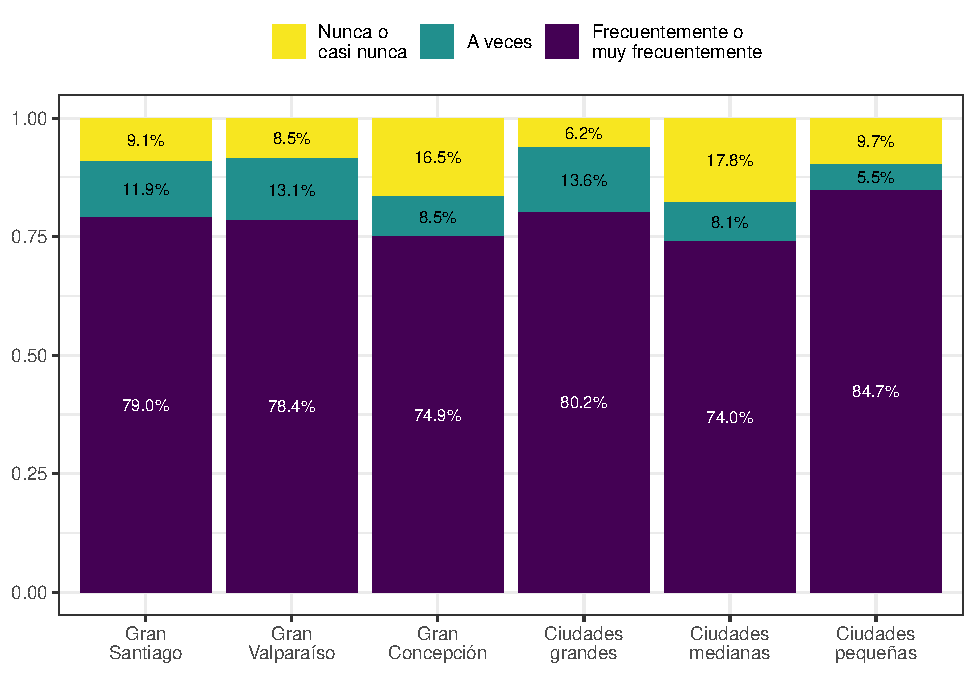
\includegraphics{reporte-elsoc_files/figure-latex/dist-estrato-1} 

}

\caption{¿En qué medida usted ha seguido la recomendación de quedarse en su hogar, manteniendo el aislamiento social? según estrato muestral (2021).}\label{fig:dist-estrato}
\end{figure}

\begin{figure}

{\centering 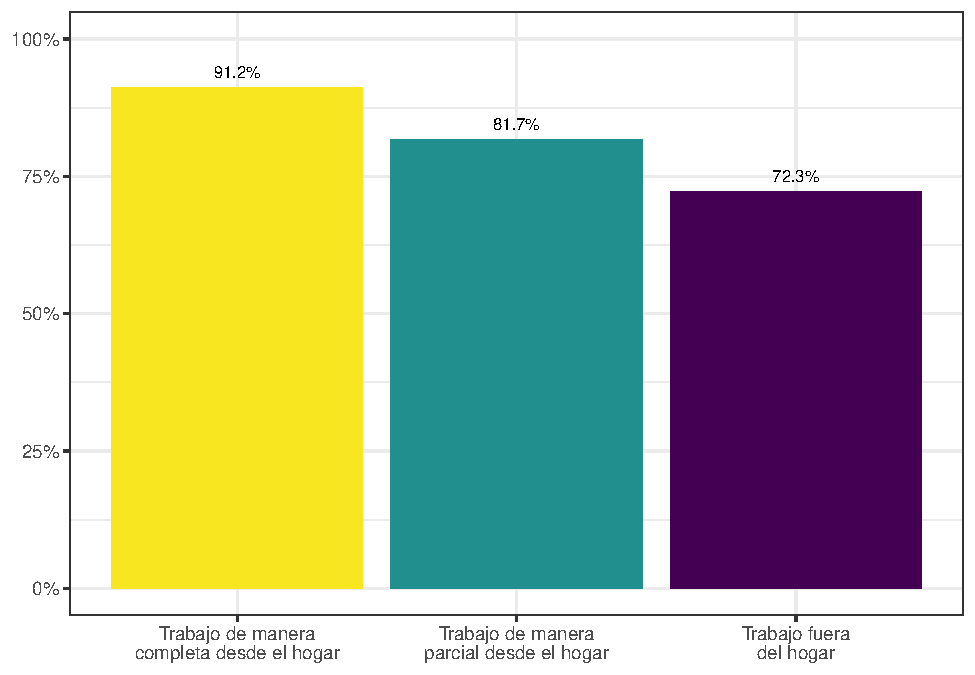
\includegraphics{reporte-elsoc_files/figure-latex/dist-telet-1} 

}

\caption{¿En qué medida usted ha seguido la recomendación de quedarse en su hogar, manteniendo el aislamiento social? según tipo de trabajo en pandemia. Suma de respuestas "Frecuente o "Muy frecuentemente" (2021).}\label{fig:dist-telet}
\end{figure}
\begin{figure}

{\centering 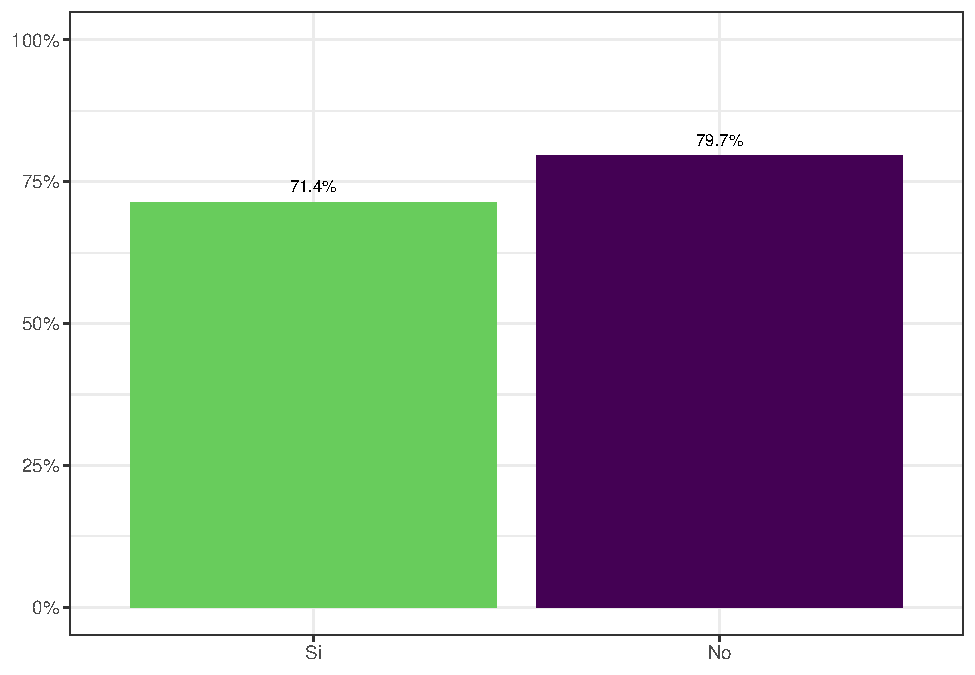
\includegraphics{reporte-elsoc_files/figure-latex/dist-covid-1} 

}

\caption{¿En qué medida usted ha seguido la recomendación de quedarse en su hogar, manteniendo el aislamiento social? según diagnóstico con coronavirus. Suma de respuestas "Frecuente o "Muy frecuentemente" (2021).}\label{fig:dist-covid}
\end{figure}

\hypertarget{efecto-del-distanciamiento-social}{%
\section{Efecto del distanciamiento social}\label{efecto-del-distanciamiento-social}}

\hypertarget{comportamiento-pro-social}{%
\subsection{Comportamiento pro-social}\label{comportamiento-pro-social}}

\begin{figure}

{\centering 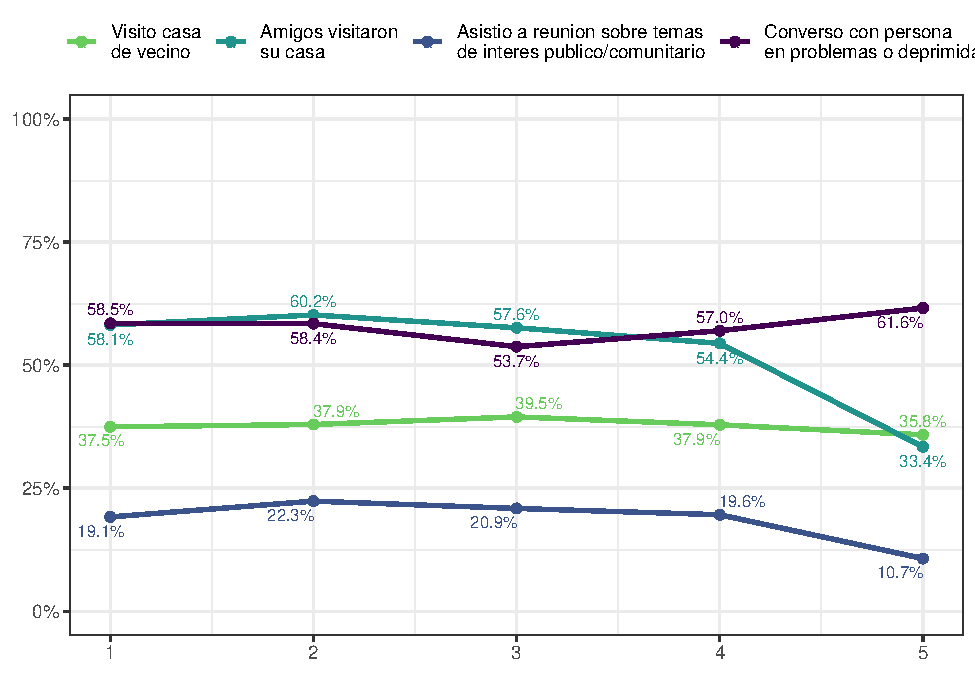
\includegraphics{reporte-elsoc_files/figure-latex/dist-pros-1} 

}

\caption{Frecuencia de comportamientos pro-sociales, según ola de estudio. Porcentaje de respuestas de "Lo hizo mas de dos veces".}\label{fig:dist-pros}
\end{figure}
\begin{figure}

{\centering \includegraphics{reporte-elsoc_files/figure-latex/dist-pros2-1} 

}

\caption{Frecuencia de comportamientos pro-sociales, según cumplimiento de distanciamiento social (2021). Porcentaje de respuestas de "Lo hizo mas de dos veces".}\label{fig:dist-pros2}
\end{figure}

\hypertarget{percepciuxf3n-de-conflictividad-y-criminalidad-barrial}{%
\subsection{Percepción de conflictividad y criminalidad barrial}\label{percepciuxf3n-de-conflictividad-y-criminalidad-barrial}}

\begin{figure}

{\centering \includegraphics{reporte-elsoc_files/figure-latex/dist-barrio-1} 

}

\caption{Percepción de conflictividad y criminalidad barrial, según cumplimiento de distanciamiento social (2021). Porcentaje de personas que responden "Muchas veces o siempre".}\label{fig:dist-barrio}
\end{figure}

\hypertarget{estatus-subjetivo-y-percepciuxf3n-de-muxe9rito}{%
\chapter{Estatus subjetivo y Percepción de Mérito}\label{estatus-subjetivo-y-percepciuxf3n-de-muxe9rito}}

\hypertarget{estatus-subjetivo}{%
\section{Estatus subjetivo}\label{estatus-subjetivo}}

\begin{figure}

{\centering \includegraphics{reporte-elsoc_files/figure-latex/ess-ola-1} 

}

\caption{En nuestra sociedad, hay grupos que tienden a ubicarse en los niveles más altos y grupos que tienden a ubicarse en los niveles más bajos de la sociedad ¿Dónde se ubicaría usted?, según ola de estudio.}\label{fig:ess-ola}
\end{figure}

\begin{figure}

{\centering \includegraphics{reporte-elsoc_files/figure-latex/ess-cambio-1} 

}

\caption{Cambios de Clase social subjetiva entre 2016, 2019 y 2021}\label{fig:ess-cambio}
\end{figure}

\begin{figure}

{\centering \includegraphics{reporte-elsoc_files/figure-latex/ess-quintil-1} 

}

\caption{Clase social subjetiva, según quintiles de ingreso (2021)}\label{fig:ess-quintil}
\end{figure}

\begin{figure}

{\centering \includegraphics{reporte-elsoc_files/figure-latex/esshijos-ess-1} 

}

\caption{Si usted tiene actualmente hijos o si los tuviera en el futuro, ¿dónde cree usted que se ubicarían ellos?, según Clase social subjetiva (2021)}\label{fig:esshijos-ess}
\end{figure}

\hypertarget{movilidad-social}{%
\section{Movilidad social}\label{movilidad-social}}

\begin{figure}

{\centering \includegraphics{reporte-elsoc_files/figure-latex/mov-soc-rec-1} 

}

\caption{Perspectiva de movilidad social, según ola.
Nota: la perspectiva de movilidad social corresponde a la resta entre el estatus social esperado del hijo y el estatus social actual del encuestado.}\label{fig:mov-soc-rec}
\end{figure}

\begin{figure}

{\centering \includegraphics{reporte-elsoc_files/figure-latex/mov-soc-1} 

}

\caption{Estatus subjetivo y tipo de movilidad social, nivel promedio según ola.
Nota: perspectiva de movilidad social corresponde a la resta entre el estatus social esperado del hijo y el estatus social actual del encuestado. En cambio movilidad social relativa corresponde a la resta entre el estatus social actual y el estatus social de la familia donde creció.}\label{fig:mov-soc}
\end{figure}

\hypertarget{percepciuxf3n-de-meritocracia}{%
\section{Percepción de meritocracia}\label{percepciuxf3n-de-meritocracia}}

\begin{figure}

{\centering \includegraphics{reporte-elsoc_files/figure-latex/merit-wave-1} 

}

\caption{Percepción de importancia y recompensas del mérito, según ola de estudio. Porcentaje de Respuestas "De acuerdo" y ”Totalmente de acuerdo".}\label{fig:merit-wave}
\end{figure}

\hypertarget{guxe9nero}{%
\chapter{Género}\label{guxe9nero}}

\hypertarget{sexismo-hostil-y-benevolente}{%
\section{Sexismo hostil y benevolente}\label{sexismo-hostil-y-benevolente}}

\begin{figure}

{\centering \includegraphics{reporte-elsoc_files/figure-latex/sexismo-sexo-1} 

}

\caption{Sexismo benévolo y hostil, según sexo (2021). Porcentaje que responde "De acuerdo" o "Totalmente de acuerdo".}\label{fig:sexismo-sexo}
\end{figure}

\begin{figure}

{\centering \includegraphics{reporte-elsoc_files/figure-latex/sexismo-educ-1} 

}

\caption{Sexismo benévolo y hostil, según nivel educacional (2021). Porcentaje que responde "De acuerdo" o "Totalmente de acuerdo".}\label{fig:sexismo-educ}
\end{figure}

\hypertarget{trabajo-y-guxe9nero}{%
\section{Trabajo y género}\label{trabajo-y-guxe9nero}}

\begin{figure}

{\centering \includegraphics{reporte-elsoc_files/figure-latex/ocup-sexo-1} 

}

\caption{Porcentaje de trabajadores y trabajadoras por situación ocupacional (2021), según sexo del entrevistado}\label{fig:ocup-sexo}
\end{figure}

\hypertarget{salud-mental-y-bienestar}{%
\chapter{Salud mental y bienestar}\label{salud-mental-y-bienestar}}

\begin{figure}

{\centering \includegraphics{reporte-elsoc_files/figure-latex/depre-wave-1} 

}

\caption{Síntomas de Depresión, según Ola del Estudio}\label{fig:depre-wave}
\end{figure}

\begin{figure}

{\centering \includegraphics{reporte-elsoc_files/figure-latex/depre-deuda-wave-1} 

}

\caption{Síntomas de Depresión, según Ola del Estudio y Sobrecarga de Deuda}\label{fig:depre-deuda-wave}
\end{figure}

\hypertarget{brecha-de-guxe9nero-en-salud-mental}{%
\section{Brecha de género en Salud Mental}\label{brecha-de-guxe9nero-en-salud-mental}}

\begin{figure}

{\centering \includegraphics{reporte-elsoc_files/figure-latex/depre-year-sexo-1} 

}

\caption{Sintomatología Depresiva por año, según sexo. Porcentaje con síntomas de “Depresion Moderada” o “Depresion Moderada Severa a Severa”.}\label{fig:depre-year-sexo}
\end{figure}

\begin{figure}

{\centering \includegraphics{reporte-elsoc_files/figure-latex/depre-sexo-1} 

}

\caption{Cambios en Síntomas de depresión entre años 2018 y 2021, según sexo}\label{fig:depre-sexo}
\end{figure}

\begin{figure}

{\centering \includegraphics{reporte-elsoc_files/figure-latex/depre-edad-sexo-1} 

}

\caption{Síntomas de Depresión según tramos de edad y sexo (2021). Porcentaje con síntomas de “Depresion Moderada” o “Depresion Moderada Severa a Severa}\label{fig:depre-edad-sexo}
\end{figure}

\hypertarget{sintomatologuxeda-depresiva-sexo-y-ocupaciuxf3n}{%
\section{Sintomatología depresiva, sexo y ocupación}\label{sintomatologuxeda-depresiva-sexo-y-ocupaciuxf3n}}

\begin{figure}

{\centering \includegraphics{reporte-elsoc_files/figure-latex/depre-labstat-1} 

}

\caption{Síntomas de Depresión según sexo y situación ocupacional (2021). Porcentaje con síntomas PHQ-9>10}\label{fig:depre-labstat}
\end{figure}

En 2021 no hay hombres en la categoría Trabajo doméstico no remunerado \(^{*}\)

\hypertarget{covid---19}{%
\section{COVID - 19}\label{covid---19}}

\begin{verbatim}
## 1 variables were not found in the dataset: s31
\end{verbatim}

\begin{figure}

{\centering \includegraphics{reporte-elsoc_files/figure-latex/covid-sexo-1} 

}

\caption{Sí fue diagnosticado con COVID-19, según sexo}\label{fig:covid-sexo}
\end{figure}

\begin{verbatim}
## 1 variables were not found in the dataset: phq
\end{verbatim}

\begin{figure}

{\centering \includegraphics{reporte-elsoc_files/figure-latex/depre-s03-1} 

}

\caption{Síntomas de Depresión según Estado de Salud y ola de estudio. Porcentaje con síntomas PHQ-9>10}\label{fig:depre-s03}
\end{figure}

\hypertarget{salud-mental-en-covid-19}{%
\section{Salud Mental en COVID-19}\label{salud-mental-en-covid-19}}

\begin{figure}

{\centering \includegraphics{reporte-elsoc_files/figure-latex/depre-teletrabajo-1} 

}

\caption{Síntomas de Depresión, según Modalidad de Trabajo}\label{fig:depre-teletrabajo}
\end{figure}

\begin{figure}

{\centering \includegraphics{reporte-elsoc_files/figure-latex/depre-beneficios-1} 

}

\caption{Síntomas de Depresión (2021), según sexo y acceso a beneficios}\label{fig:depre-beneficios}
\end{figure}

\begin{verbatim}
## 1 variables were not found in the dataset: phq
\end{verbatim}

\begin{figure}

{\centering \includegraphics{reporte-elsoc_files/figure-latex/depre clase.sub-1} 

}

\caption{Síntomas de Depresión, según Clase Subjetiva y ola. Porcentaje con síntomas PHQ-9>10}(\#fig:depre clase.sub)
\end{figure}

\hypertarget{migraciuxf3n}{%
\chapter{Migración}\label{migraciuxf3n}}

\hypertarget{amenaza-realista-y-amenaza-simbuxf3lica-respecto-a-inmigrantes}{%
\section{Amenaza realista y amenaza simbólica respecto a inmigrantes}\label{amenaza-realista-y-amenaza-simbuxf3lica-respecto-a-inmigrantes}}

\begin{figure}

{\centering \includegraphics{reporte-elsoc_files/figure-latex/amen1-wave-1} 

}

\caption{Con la llegada de migrantes a Chile, está aumentando el desempleo", según ola y origen de migrantes. Porcentaje de personas que responden "De acuerdo" o Totalmente de acuerdo".}\label{fig:amen1-wave}
\end{figure}

\begin{figure}

{\centering \includegraphics{reporte-elsoc_files/figure-latex/amen1-zona-1} 

}

\caption{Con la llegada de migrantes a Chile, está aumentando el desempleo", según ola, zona y origen de migrantes. Porcentaje de personas que responden "De acuerdo" o Totalmente de acuerdo".}\label{fig:amen1-zona}
\end{figure}

\begin{figure}

{\centering \includegraphics{reporte-elsoc_files/figure-latex/amen2-wave-1} 

}

\caption{"Con la llegada de migrantes, Chile está perdiendo su identidad", según ola y origen de migrantes. Porcentaje de personas que responden "De acuerdo" o "Totalmente de acuerdo".}\label{fig:amen2-wave}
\end{figure}

\begin{figure}

{\centering \includegraphics{reporte-elsoc_files/figure-latex/amen2-zona-1} 

}

\caption{"Con la llegada de migrantes, Chile está perdiendo su identidad", según ola, zona y origen de migrantes. Porcentaje de personas que responden "De acuerdo" o "Totalmente de acuerdo".}\label{fig:amen2-zona}
\end{figure}

\begin{figure}

{\centering \includegraphics{reporte-elsoc_files/figure-latex/conf-wave-1} 

}

\caption{Confianza en migrantes, según ola y origen de migrantes. Porcentaje de personas que responden “Bastante” o “Mucha confianza”}\label{fig:conf-wave}
\end{figure}

\begin{figure}

{\centering \includegraphics{reporte-elsoc_files/figure-latex/conf-zona-1} 

}

\caption{Confianza en migrantes, según ola, zona y origen de migrantes. Porcentaje de personas que responden “Bastante” o “Mucha confianza”}\label{fig:conf-zona}
\end{figure}

\begin{figure}

{\centering \includegraphics{reporte-elsoc_files/figure-latex/amen-wave-1} 

}

\caption{Percepción de amenaza realista y simbólica, según grupo de migrantes (2021). Porcentaje de personas que responden "De acuerdo" o Totalmente de acuerdo".}\label{fig:amen-wave}
\end{figure}

\hypertarget{amenaza-realista-y-simbuxf3lica-respecto-a-inmigrantes-seguxfan-nivel-educacional}{%
\section{Amenaza realista y simbólica respecto a inmigrantes según nivel educacional}\label{amenaza-realista-y-simbuxf3lica-respecto-a-inmigrantes-seguxfan-nivel-educacional}}

\begin{figure}

{\centering \includegraphics{reporte-elsoc_files/figure-latex/amen-educ-1} 

}

\caption{Percepción de amenaza realista y simbólica respecto a inmigrantes, según nivel educacional (2021). Porcentaje de personas que responden "De acuerdo" o Totalmente de acuerdo".}\label{fig:amen-educ}
\end{figure}

\begin{figure}

{\centering \includegraphics{reporte-elsoc_files/figure-latex/amen-edad-1} 

}

\caption{Percepción de amenaza realista y simbólica, según tramo de edad (2021). Porcentaje de personas que responden "De acuerdo" o Totalmente de acuerdo".}\label{fig:amen-edad}
\end{figure}

\hypertarget{pandemia-covid-19}{%
\chapter{Pandemia Covid-19}\label{pandemia-covid-19}}

\hypertarget{cuarentenas}{%
\section{Cuarentenas}\label{cuarentenas}}

\begin{figure}

{\centering \includegraphics{reporte-elsoc_files/figure-latex/hist-fecha-2021-1} 

}

\caption{Histograma Fechas de Entrevistas}\label{fig:hist-fecha-2021}
\end{figure}

\begin{figure}

{\centering \includegraphics{reporte-elsoc_files/figure-latex/ccum-heter-1} 

}

\caption{Heterogeneidad de Cuarentena Acumulada en el Panel}\label{fig:ccum-heter}
\end{figure}

\begin{figure}

{\centering \includegraphics{reporte-elsoc_files/figure-latex/ccum-zona-1} 

}

\caption{Días de Cuarentena Acumulada al momento de la entrevista, según Zona}\label{fig:ccum-zona}
\end{figure}

\begin{figure}

{\centering \includegraphics{reporte-elsoc_files/figure-latex/ccum-edad-1} 

}

\caption{Días de Cuarentena Acumulada al momento de la entrevista, según Tramo Etario}\label{fig:ccum-edad}
\end{figure}

\begin{figure}

{\centering \includegraphics{reporte-elsoc_files/figure-latex/ccum-aislamiento-1} 

}

\caption{Cumplimiento de Aislamiento Social, según Días de Cuarentena Acumulada al momento de la entrevista}\label{fig:ccum-aislamiento}
\end{figure}

\begin{verbatim}
## 1 variables were not found in the dataset: phq
\end{verbatim}

\begin{figure}

{\centering \includegraphics{reporte-elsoc_files/figure-latex/ccum-depr-1} 

}

\caption{Sintomatología Depresiva, según Días de Cuarentena Acumulada al momento de la entrevista}\label{fig:ccum-depr}
\end{figure}

\textbackslash begin\{figure\}

\{\centering \includegraphics{reporte-elsoc_files/figure-latex/ccum-sit_ocup-1}

\}

\caption{Situación Ocupacional, según Días de Cuarentena Acumulada al momento de la entrevista}

(\#fig:ccum-sit\_ocup)
\textbackslash end\{figure\}

\begin{verbatim}
## 1 variables were not found in the dataset: m44_rec
\end{verbatim}

\begin{figure}

{\centering \includegraphics{reporte-elsoc_files/figure-latex/ccum-ahorro-1} 

}

\caption{Nivel de Ahorro "Nada o Poco", según Días de Cuarentena Acumulada al momento de la entrevista (2021)}\label{fig:ccum-ahorro}
\end{figure}

\begin{figure}

{\centering \includegraphics{reporte-elsoc_files/figure-latex/cuarentena-etario-1} 

}

\caption{Encuestados en Cuarentena según Tramo Etario}\label{fig:cuarentena-etario}
\end{figure}

\hypertarget{estruxe9s-financiero}{%
\section{Estrés Financiero}\label{estruxe9s-financiero}}

\begin{figure}

{\centering \includegraphics{reporte-elsoc_files/figure-latex/satisfaccion-wave-1} 

}

\caption{Satisfacción con el Ingreso por Ola}\label{fig:satisfaccion-wave}
\end{figure}

\begin{figure}

{\centering \includegraphics{reporte-elsoc_files/figure-latex/satisfaccion-retiro-1} 

}

\caption{Satisfacción con el Ingreso según Retiro AFP}\label{fig:satisfaccion-retiro}
\end{figure}

\begin{figure}

{\centering \includegraphics{reporte-elsoc_files/figure-latex/clase.sub-benef.estatal-1} 

}

\caption{Satisfacción con el Ingreso según Acceso a Beneficios}(\#fig:clase.sub-benef.estatal)
\end{figure}

\begin{figure}

{\centering \includegraphics{reporte-elsoc_files/figure-latex/clase.sub.hij-1erretiro-1} 

}

\caption{Clase Social Subjetiva de Hijo según Primer Retiro AFP}(\#fig:clase.sub.hij-1erretiro)
\end{figure}

\begin{figure}

{\centering \includegraphics{reporte-elsoc_files/figure-latex/endeud-1retiro-1} 

}

\caption{Sobrecarga de Deuda según Primer Retiro AFP}\label{fig:endeud-1retiro}
\end{figure}

\begin{figure}

{\centering \includegraphics{reporte-elsoc_files/figure-latex/endeud-2retiro-1} 

}

\caption{Sobrecarga de Deuda según Primer Retiro AFP}\label{fig:endeud-2retiro}
\end{figure}

\begin{figure}

{\centering \includegraphics{reporte-elsoc_files/figure-latex/deuda-retiro1-1} 

}

\caption{Primer retiro de AFP, según deuda}\label{fig:deuda-retiro1}
\end{figure}

\begin{figure}

{\centering \includegraphics{reporte-elsoc_files/figure-latex/deuda-retiro2-1} 

}

\caption{Segundo retiro de AFP, según deuda}\label{fig:deuda-retiro2}
\end{figure}

\begin{figure}

{\centering \includegraphics{reporte-elsoc_files/figure-latex/deuda-benef-1} 

}

\caption{Beneficios Estatales, según deuda}\label{fig:deuda-benef}
\end{figure}

\hypertarget{cuxf3mo-citar-este-informe}{%
\chapter*{Cómo citar este informe:}\label{cuxf3mo-citar-este-informe}}
\addcontentsline{toc}{chapter}{Cómo citar este informe:}

\begin{quote}
COES (2021) Radiografía del Cambio Social: Análisis de Resultados Longitudinales ELSOC 2016-2021. Presentación de Resultados COES. Septiembre, Santiago de Chile.
\end{quote}

\textbf{Entrada Bibtex:}

\begin{Shaded}
\begin{Highlighting}[]
\SpecialCharTok{@}\NormalTok{techreport\{coes\_Radiografia\_2021,}
\NormalTok{  title }\OtherTok{=}\NormalTok{ \{Radiograf\textbackslash{}}\StringTok{\textquotesingle{}ia Del \{\{Cambio Social\}\}: \{\{An}\SpecialCharTok{\textbackslash{}\textquotesingle{}}\StringTok{alisis\}\} de \{\{Resultados Longitudinales ELSOC\}\} 2016{-}2021.\},}
\StringTok{  author = \{COES\},}
\StringTok{  year = \{2021\},}
\StringTok{  month = sep,}
\StringTok{  address = \{\{Santiago de Chile, Chile\}\},}
\StringTok{  institution = \{\{Centro de Estudios de Conflicto y Cohesi}\SpecialCharTok{\textbackslash{}\textquotesingle{}}\StringTok{on Social\}\}}
\StringTok{\}}
\end{Highlighting}
\end{Shaded}


\end{document}
